\documentclass[twoside]{book}

% Packages required by doxygen
\usepackage{fixltx2e}
\usepackage{calc}
\usepackage{doxygen}
\usepackage[export]{adjustbox} % also loads graphicx
\usepackage{graphicx}
\usepackage[utf8]{inputenc}
\usepackage{makeidx}
\usepackage{multicol}
\usepackage{multirow}
\PassOptionsToPackage{warn}{textcomp}
\usepackage{textcomp}
\usepackage[nointegrals]{wasysym}
\usepackage[table]{xcolor}

% Font selection
\usepackage[T1]{fontenc}
\usepackage[scaled=.90]{helvet}
\usepackage{courier}
\usepackage{amssymb}
\usepackage{sectsty}
\renewcommand{\familydefault}{\sfdefault}
\allsectionsfont{%
  \fontseries{bc}\selectfont%
  \color{darkgray}%
}
\renewcommand{\DoxyLabelFont}{%
  \fontseries{bc}\selectfont%
  \color{darkgray}%
}
\newcommand{\+}{\discretionary{\mbox{\scriptsize$\hookleftarrow$}}{}{}}

% Page & text layout
\usepackage{geometry}
\geometry{%
  a4paper,%
  top=2.5cm,%
  bottom=2.5cm,%
  left=2.5cm,%
  right=2.5cm%
}
\tolerance=750
\hfuzz=15pt
\hbadness=750
\setlength{\emergencystretch}{15pt}
\setlength{\parindent}{0cm}
\setlength{\parskip}{0.2cm}
\makeatletter
\renewcommand{\paragraph}{%
  \@startsection{paragraph}{4}{0ex}{-1.0ex}{1.0ex}{%
    \normalfont\normalsize\bfseries\SS@parafont%
  }%
}
\renewcommand{\subparagraph}{%
  \@startsection{subparagraph}{5}{0ex}{-1.0ex}{1.0ex}{%
    \normalfont\normalsize\bfseries\SS@subparafont%
  }%
}
\makeatother

% Headers & footers
\usepackage{fancyhdr}
\pagestyle{fancyplain}
\fancyhead[LE]{\fancyplain{}{\bfseries\thepage}}
\fancyhead[CE]{\fancyplain{}{}}
\fancyhead[RE]{\fancyplain{}{\bfseries\leftmark}}
\fancyhead[LO]{\fancyplain{}{\bfseries\rightmark}}
\fancyhead[CO]{\fancyplain{}{}}
\fancyhead[RO]{\fancyplain{}{\bfseries\thepage}}
\fancyfoot[LE]{\fancyplain{}{}}
\fancyfoot[CE]{\fancyplain{}{}}
\fancyfoot[RE]{\fancyplain{}{\bfseries\scriptsize Generated on Tue Oct 6 2015 11\+:20\+:57 for A\+S\+T\+L by Doxygen }}
\fancyfoot[LO]{\fancyplain{}{\bfseries\scriptsize Generated on Tue Oct 6 2015 11\+:20\+:57 for A\+S\+T\+L by Doxygen }}
\fancyfoot[CO]{\fancyplain{}{}}
\fancyfoot[RO]{\fancyplain{}{}}
\renewcommand{\footrulewidth}{0.4pt}
\renewcommand{\chaptermark}[1]{%
  \markboth{#1}{}%
}
\renewcommand{\sectionmark}[1]{%
  \markright{\thesection\ #1}%
}

% Indices & bibliography
\usepackage{natbib}
\usepackage[titles]{tocloft}
\setcounter{tocdepth}{3}
\setcounter{secnumdepth}{5}
\makeindex

% Custom commands
\newcommand{\clearemptydoublepage}{%
  \newpage{\pagestyle{empty}\cleardoublepage}%
}


%===== C O N T E N T S =====

\begin{document}

% Titlepage & ToC
\pagenumbering{roman}
\begin{titlepage}
\vspace*{7cm}
\begin{center}%
{\Large A\+S\+T\+L \\[1ex]\large 2.\+0.\+0 }\\
\vspace*{1cm}
{\large Generated by Doxygen 1.8.9.1}\\
\vspace*{0.5cm}
{\small Tue Oct 6 2015 11:20:57}\\
\end{center}
\end{titlepage}
\clearemptydoublepage
\tableofcontents
\clearemptydoublepage
\pagenumbering{arabic}

%--- Begin generated contents ---
\chapter{Hierarchical Index}
\section{Class Hierarchy}
This inheritance list is sorted roughly, but not completely, alphabetically\+:\begin{DoxyCompactList}
\item C\+H\+A\+R\+\_\+\+T\+R\+A\+I\+TS\begin{DoxyCompactList}
\item \contentsline{section}{Net\+Transition}{\pageref{class_net_transition}}{}
\begin{DoxyCompactList}
\item \contentsline{section}{Sys\+Transition}{\pageref{class_sys_transition}}{}
\end{DoxyCompactList}
\item \contentsline{section}{Transition}{\pageref{class_transition}}{}
\end{DoxyCompactList}
\item \contentsline{section}{Component\+Model}{\pageref{class_component_model}}{}
\item \contentsline{section}{Net\+Component}{\pageref{class_net_component}}{}
\begin{DoxyCompactList}
\item \contentsline{section}{Component}{\pageref{class_component}}{}
\end{DoxyCompactList}
\item \contentsline{section}{Network\+Model}{\pageref{class_network_model}}{}
\item \contentsline{section}{Pattern}{\pageref{class_pattern}}{}
\item \contentsline{section}{Problem}{\pageref{class_problem}}{}
\item \contentsline{section}{Problem\+Node}{\pageref{class_problem_node}}{}
\item \contentsline{section}{State\+Data\+\_\+str}{\pageref{class_state_data__str}}{}
\item \contentsline{section}{State\+Data\+\_\+str\+List}{\pageref{class_state_data__str_list}}{}
\item \contentsline{section}{System}{\pageref{class_system}}{}
\item \contentsline{section}{System\+Node}{\pageref{class_system_node}}{}
\item \contentsline{section}{Terminal}{\pageref{class_terminal}}{}
\item \contentsline{section}{Utils}{\pageref{class_utils}}{}
\end{DoxyCompactList}

\chapter{Class Index}
\section{Class List}
Here are the classes, structs, unions and interfaces with brief descriptions\+:\begin{DoxyCompactList}
\item\contentsline{section}{\hyperlink{structyy_1_1spec__parser_1_1basic__symbol}{yy\+::spec\+\_\+parser\+::basic\+\_\+symbol$<$ Base $>$} }{\pageref{structyy_1_1spec__parser_1_1basic__symbol}}{}
\item\contentsline{section}{\hyperlink{structyy_1_1spec__parser_1_1by__type}{yy\+::spec\+\_\+parser\+::by\+\_\+type} \\*Type access provider for token (enum) based symbols }{\pageref{structyy_1_1spec__parser_1_1by__type}}{}
\item\contentsline{section}{\hyperlink{classyy_1_1location}{yy\+::location} \\*Abstract a location }{\pageref{classyy_1_1location}}{}
\item\contentsline{section}{\hyperlink{classyy_1_1position}{yy\+::position} \\*Abstract a position }{\pageref{classyy_1_1position}}{}
\item\contentsline{section}{\hyperlink{classyy_1_1slice}{yy\+::slice$<$ T, S $>$} \\*Present a slice of the top of a stack }{\pageref{classyy_1_1slice}}{}
\item\contentsline{section}{\hyperlink{classspec__driver}{spec\+\_\+driver} \\*The \hyperlink{classspec__driver}{spec\+\_\+driver} class\+: sintax analysis and semantics driver class }{\pageref{classspec__driver}}{}
\item\contentsline{section}{\hyperlink{classyy_1_1spec__parser}{yy\+::spec\+\_\+parser} \\*A Bison parser }{\pageref{classyy_1_1spec__parser}}{}
\item\contentsline{section}{\hyperlink{classyy_1_1stack}{yy\+::stack$<$ T, S $>$} }{\pageref{classyy_1_1stack}}{}
\item\contentsline{section}{\hyperlink{structyy_1_1spec__parser_1_1syntax__error}{yy\+::spec\+\_\+parser\+::syntax\+\_\+error} \\*Syntax errors thrown from user actions }{\pageref{structyy_1_1spec__parser_1_1syntax__error}}{}
\item\contentsline{section}{\hyperlink{structyy_1_1spec__parser_1_1token}{yy\+::spec\+\_\+parser\+::token} \\*Tokens }{\pageref{structyy_1_1spec__parser_1_1token}}{}
\item\contentsline{section}{\hyperlink{unionyy_1_1spec__parser_1_1union__type}{yy\+::spec\+\_\+parser\+::union\+\_\+type} \\*An auxiliary type to compute the largest semantic type }{\pageref{unionyy_1_1spec__parser_1_1union__type}}{}
\item\contentsline{section}{\hyperlink{structyy_1_1variant}{yy\+::variant$<$ S $>$} }{\pageref{structyy_1_1variant}}{}
\item\contentsline{section}{\hyperlink{structyy__buffer__state}{yy\+\_\+buffer\+\_\+state} }{\pageref{structyy__buffer__state}}{}
\item\contentsline{section}{\hyperlink{structyy__trans__info}{yy\+\_\+trans\+\_\+info} }{\pageref{structyy__trans__info}}{}
\end{DoxyCompactList}

\chapter{File Index}
\section{File List}
Here is a list of all documented files with brief descriptions\+:\begin{DoxyCompactList}
\item\contentsline{section}{{\bfseries aho\+\_\+corasick.\+h} }{\pageref{aho__corasick_8h}}{}
\item\contentsline{section}{{\bfseries alphabet.\+h} }{\pageref{alphabet_8h}}{}
\item\contentsline{section}{{\bfseries astl.\+h} }{\pageref{astl_8h}}{}
\item\contentsline{section}{{\bfseries build.\+h} }{\pageref{build_8h}}{}
\item\contentsline{section}{{\bfseries capture.\+h} }{\pageref{capture_8h}}{}
\item\contentsline{section}{{\bf ccopy.\+h} }{\pageref{ccopy_8h}}{}
\item\contentsline{section}{{\bfseries check.\+h} }{\pageref{check_8h}}{}
\item\contentsline{section}{{\bfseries closure.\+h} }{\pageref{closure_8h}}{}
\item\contentsline{section}{{\bfseries combinatory.\+h} }{\pageref{combinatory_8h}}{}
\item\contentsline{section}{{\bfseries concept.\+h} }{\pageref{concept_8h}}{}
\item\contentsline{section}{{\bf cursor.\+h} }{\pageref{cursor_8h}}{}
\item\contentsline{section}{{\bfseries debug.\+h} }{\pageref{debug_8h}}{}
\item\contentsline{section}{{\bfseries default.\+h} }{\pageref{default_8h}}{}
\item\contentsline{section}{{\bfseries determinize.\+h} }{\pageref{determinize_8h}}{}
\item\contentsline{section}{{\bfseries dfa.\+h} }{\pageref{dfa_8h}}{}
\item\contentsline{section}{{\bfseries dfa\+\_\+base.\+h} }{\pageref{dfa__base_8h}}{}
\item\contentsline{section}{{\bfseries dfa\+\_\+bin.\+h} }{\pageref{dfa__bin_8h}}{}
\item\contentsline{section}{{\bfseries dfa\+\_\+compact.\+h} }{\pageref{dfa__compact_8h}}{}
\item\contentsline{section}{{\bfseries dfa\+\_\+hash.\+h} }{\pageref{dfa__hash_8h}}{}
\item\contentsline{section}{{\bfseries dfa\+\_\+map.\+h} }{\pageref{dfa__map_8h}}{}
\item\contentsline{section}{{\bfseries dfa\+\_\+matrix.\+h} }{\pageref{dfa__matrix_8h}}{}
\item\contentsline{section}{{\bfseries dfa\+\_\+min.\+h} }{\pageref{dfa__min_8h}}{}
\item\contentsline{section}{{\bfseries dfa\+\_\+min\+\_\+hash.\+h} }{\pageref{dfa__min__hash_8h}}{}
\item\contentsline{section}{{\bfseries dfa\+\_\+mtf.\+h} }{\pageref{dfa__mtf_8h}}{}
\item\contentsline{section}{{\bfseries dfa\+\_\+tr.\+h} }{\pageref{dfa__tr_8h}}{}
\item\contentsline{section}{{\bfseries dir\+\_\+cursor.\+h} }{\pageref{dir__cursor_8h}}{}
\item\contentsline{section}{{\bfseries dot.\+h} }{\pageref{dot_8h}}{}
\item\contentsline{section}{{\bfseries experiment.\+h} }{\pageref{experiment_8h}}{}
\item\contentsline{section}{{\bfseries fa\+\_\+compress.\+h} }{\pageref{fa__compress_8h}}{}
\item\contentsline{section}{{\bfseries filter.\+h} }{\pageref{filter_8h}}{}
\item\contentsline{section}{{\bfseries hash.\+h} }{\pageref{hash_8h}}{}
\item\contentsline{section}{{\bfseries language.\+h} }{\pageref{language_8h}}{}
\item\contentsline{section}{{\bfseries lazy.\+h} }{\pageref{lazy_8h}}{}
\item\contentsline{section}{{\bf match.\+h} }{\pageref{match_8h}}{}
\item\contentsline{section}{{\bfseries minimize.\+h} }{\pageref{minimize_8h}}{}
\item\contentsline{section}{{\bfseries namespace.\+h} }{\pageref{namespace_8h}}{}
\item\contentsline{section}{{\bfseries neighbor.\+h} }{\pageref{neighbor_8h}}{}
\item\contentsline{section}{{\bfseries nfa\+\_\+epsilon.\+h} }{\pageref{nfa__epsilon_8h}}{}
\item\contentsline{section}{{\bfseries nfa\+\_\+mmap.\+h} }{\pageref{nfa__mmap_8h}}{}
\item\contentsline{section}{{\bfseries random.\+h} }{\pageref{random_8h}}{}
\item\contentsline{section}{{\bfseries regexp.\+h} }{\pageref{regexp_8h}}{}
\item\contentsline{section}{{\bfseries set\+\_\+operation.\+h} }{\pageref{set__operation_8h}}{}
\item\contentsline{section}{{\bfseries state.\+h} }{\pageref{state_8h}}{}
\item\contentsline{section}{{\bfseries stats.\+h} }{\pageref{stats_8h}}{}
\item\contentsline{section}{{\bfseries str\+\_\+cursor.\+h} }{\pageref{str__cursor_8h}}{}
\item\contentsline{section}{{\bfseries stream.\+h} }{\pageref{stream_8h}}{}
\item\contentsline{section}{{\bfseries tag.\+h} }{\pageref{tag_8h}}{}
\item\contentsline{section}{{\bfseries tools.\+h} }{\pageref{tools_8h}}{}
\end{DoxyCompactList}

\chapter{Class Documentation}
\section{bfirst\+\_\+cursor$<$ Queue\+Cursor, Marker\+Function $>$ Class Template Reference}
\label{classastl_1_1bfirst__cursor}\index{bfirst\+\_\+cursor$<$ Queue\+Cursor, Marker\+Function $>$@{bfirst\+\_\+cursor$<$ Queue\+Cursor, Marker\+Function $>$}}


A \doxyref{bfirst\+\_\+cursor}{p.}{classastl_1_1bfirst__cursor_a43b959e39feac33b5c81a1ca84ca7282} implements the breadth-\/first traversal on deterministic automata.  




{\ttfamily \#include $<$cursor.\+h$>$}



Inherits bfirst\+\_\+cursor\+\_\+concept.

\subsection*{Public Types}
\begin{DoxyCompactItemize}
\item 
typedef Queue\+Cursor\+::char\+\_\+traits {\bf char\+\_\+traits}\label{classastl_1_1bfirst__cursor_a66e94af01b68f4ddbdb9d11e8fd5596e}

\begin{DoxyCompactList}\small\item\em Character traits describing \doxyref{char\+\_\+type}{p.}{classastl_1_1bfirst__cursor_a2e0f3aa50487d878b4688afd95cc093c}. \end{DoxyCompactList}\item 
typedef Queue\+Cursor\+::char\+\_\+type {\bf char\+\_\+type}\label{classastl_1_1bfirst__cursor_a2e0f3aa50487d878b4688afd95cc093c}

\begin{DoxyCompactList}\small\item\em The type of the transitions letters. \end{DoxyCompactList}\item 
typedef Queue\+Cursor\+::state\+\_\+type {\bf state\+\_\+type}\label{classastl_1_1bfirst__cursor_a86ea628a39e2fc04a741886783de367e}

\begin{DoxyCompactList}\small\item\em The type of the automaton-\/states identifiers. \end{DoxyCompactList}\item 
typedef Queue\+Cursor\+::tag\+\_\+type {\bf tag\+\_\+type}\label{classastl_1_1bfirst__cursor_a9427e44e81e59f72ffc04356531d6e1f}

\begin{DoxyCompactList}\small\item\em The type of the data attached to states. \end{DoxyCompactList}\end{DoxyCompactItemize}
\subsection*{Public Member Functions}
\begin{DoxyCompactItemize}
\item 
{\bf state\+\_\+type} {\bf aim} () const 
\begin{DoxyCompactList}\small\item\em Returns the aim state of the pointed transition. \end{DoxyCompactList}\item 
bool {\bf aim\+\_\+final} () const 
\begin{DoxyCompactList}\small\item\em Returns {\ttfamily true} if the aim state of the transition that this cursor points to is final. \end{DoxyCompactList}\item 
{\bf tag\+\_\+type} {\bf aim\+\_\+tag} () const 
\begin{DoxyCompactList}\small\item\em Returns the data attached to the aim state of the pointed transition. \end{DoxyCompactList}\item 
{\bf bfirst\+\_\+cursor} (const Queue\+Cursor \&x, const Marker\+Function \&f=Marker\+Function())\label{classastl_1_1bfirst__cursor_a43b959e39feac33b5c81a1ca84ca7282}

\begin{DoxyCompactList}\small\item\em Creates a cursor with {\ttfamily x} as queue. \end{DoxyCompactList}\item 
{\bf bfirst\+\_\+cursor} ()\label{classastl_1_1bfirst__cursor_af626ca74d4cdd2b69a8bce2b5dc1d3b2}

\begin{DoxyCompactList}\small\item\em Creates a cursor with an empty queue used as an end-\/of-\/range iterator. \end{DoxyCompactList}\item 
{\bf char\+\_\+type} {\bf letter} () const 
\begin{DoxyCompactList}\small\item\em Returns the letter on the pointed transition. \end{DoxyCompactList}\item 
bool {\bf next} ()
\begin{DoxyCompactList}\small\item\em Increments the cursor making it point to the next transition in the sequence. \end{DoxyCompactList}\item 
bool {\bf operator!=} (const {\bf self} \&x) const 
\begin{DoxyCompactList}\small\item\em Returns {\ttfamily true} if queues are different compared element by element. \end{DoxyCompactList}\item 
bool {\bf operator==} (const {\bf self} \&x) const 
\begin{DoxyCompactList}\small\item\em Returns {\ttfamily true} if both queues are equal compared element by element. \end{DoxyCompactList}\item 
{\bf state\+\_\+type} {\bf src} () const 
\begin{DoxyCompactList}\small\item\em Returns the identifier of the state that this cursor points to. \end{DoxyCompactList}\item 
bool {\bf src\+\_\+final} () const 
\begin{DoxyCompactList}\small\item\em Returns {\ttfamily true} if the state that this cursor points to is final. \end{DoxyCompactList}\item 
{\bf tag\+\_\+type} {\bf src\+\_\+tag} () const 
\begin{DoxyCompactList}\small\item\em Returns the data attached to the state that this cursor points to. \end{DoxyCompactList}\end{DoxyCompactItemize}


\subsection{Detailed Description}
\subsubsection*{template$<$typename Queue\+Cursor, typename Marker\+Function = none$>$class astl\+::bfirst\+\_\+cursor$<$ Queue\+Cursor, Marker\+Function $>$}

A \doxyref{bfirst\+\_\+cursor}{p.}{classastl_1_1bfirst__cursor_a43b959e39feac33b5c81a1ca84ca7282} implements the breadth-\/first traversal on deterministic automata. 

It is an iterator on a sequence of transitions ordered according to the breadth-\/first traversal algorithm. The method \doxyref{next()}{p.}{classastl_1_1bfirst__cursor_a80870c233d0237e3588a2d6f8d176916} allows to increment the cursor, making it point to the next transition in the sequence. This methods returns {\ttfamily true} if the transition reached has been enqueued and {\ttfamily false} otherwise (dequeue). The \doxyref{bfirst\+\_\+cursor}{p.}{classastl_1_1bfirst__cursor} is used in the same way as the iterators on sequence to define ranges foralgorithms. \begin{DoxyParagraph}{Template parameters}
\begin{TabularC}{4}
\hline
\rowcolor{lightgray}{\bf Parameter}&{\bf Description}&{\bf Default}&{\bf Requirements }\\\cline{1-4}
{\ttfamily Queue\+Cursor} &The type of the queue cursor&&{\ttfamily Queue\+Cursor} is a model of queue cursor \\\cline{1-4}
{\ttfamily Marker\+Function} &The type of state marker used for preventing the cursor from visiting twice the same transition on cyclic automata and D\+A\+Gs&{\ttfamily none} &{\ttfamily Marker\+Function} is either {\ttfamily none}, {\ttfamily set\+\_\+marker$<$\+Forward\+Cursor\+::state\+\_\+type$>$} or a model of state marker\\\cline{1-4}
\end{TabularC}

\end{DoxyParagraph}
\begin{DoxyParagraph}{Model of}
\doxyref{bfirst\+\_\+cursor}{p.}{classastl_1_1bfirst__cursor_a43b959e39feac33b5c81a1ca84ca7282} 
\end{DoxyParagraph}
\begin{DoxyParagraph}{Associated Helper Functions}
bfirstc(), bfirst\+\_\+markc() 
\end{DoxyParagraph}


\subsection{Member Function Documentation}
\index{astl\+::bfirst\+\_\+cursor@{astl\+::bfirst\+\_\+cursor}!aim@{aim}}
\index{aim@{aim}!astl\+::bfirst\+\_\+cursor@{astl\+::bfirst\+\_\+cursor}}
\subsubsection[{aim}]{\setlength{\rightskip}{0pt plus 5cm}{\bf state\+\_\+type} aim (
\begin{DoxyParamCaption}
{}
\end{DoxyParamCaption}
) const}\label{classastl_1_1bfirst__cursor_a742bd0e539b1f9df56841304b7ef4272}


Returns the aim state of the pointed transition. 

\begin{DoxyPrecond}{Precondition}
The queue is not empty 
\end{DoxyPrecond}
\index{astl\+::bfirst\+\_\+cursor@{astl\+::bfirst\+\_\+cursor}!aim\+\_\+final@{aim\+\_\+final}}
\index{aim\+\_\+final@{aim\+\_\+final}!astl\+::bfirst\+\_\+cursor@{astl\+::bfirst\+\_\+cursor}}
\subsubsection[{aim\+\_\+final}]{\setlength{\rightskip}{0pt plus 5cm}bool aim\+\_\+final (
\begin{DoxyParamCaption}
{}
\end{DoxyParamCaption}
) const}\label{classastl_1_1bfirst__cursor_a8fdf66e2483d23e73580e5c9ed937dfb}


Returns {\ttfamily true} if the aim state of the transition that this cursor points to is final. 

\begin{DoxyPrecond}{Precondition}
The queue is not empty 
\end{DoxyPrecond}
\index{astl\+::bfirst\+\_\+cursor@{astl\+::bfirst\+\_\+cursor}!aim\+\_\+tag@{aim\+\_\+tag}}
\index{aim\+\_\+tag@{aim\+\_\+tag}!astl\+::bfirst\+\_\+cursor@{astl\+::bfirst\+\_\+cursor}}
\subsubsection[{aim\+\_\+tag}]{\setlength{\rightskip}{0pt plus 5cm}{\bf tag\+\_\+type} aim\+\_\+tag (
\begin{DoxyParamCaption}
{}
\end{DoxyParamCaption}
) const}\label{classastl_1_1bfirst__cursor_a76a01210687f95ea151f8073a0eac35f}


Returns the data attached to the aim state of the pointed transition. 

\begin{DoxyPrecond}{Precondition}
The queue is not empty 
\end{DoxyPrecond}
\index{astl\+::bfirst\+\_\+cursor@{astl\+::bfirst\+\_\+cursor}!letter@{letter}}
\index{letter@{letter}!astl\+::bfirst\+\_\+cursor@{astl\+::bfirst\+\_\+cursor}}
\subsubsection[{letter}]{\setlength{\rightskip}{0pt plus 5cm}{\bf char\+\_\+type} letter (
\begin{DoxyParamCaption}
{}
\end{DoxyParamCaption}
) const}\label{classastl_1_1bfirst__cursor_a6b28dc14fee32fdbd1e558b9c4884c9f}


Returns the letter on the pointed transition. 

\begin{DoxyPrecond}{Precondition}
The queue is not empty 
\end{DoxyPrecond}
\index{astl\+::bfirst\+\_\+cursor@{astl\+::bfirst\+\_\+cursor}!next@{next}}
\index{next@{next}!astl\+::bfirst\+\_\+cursor@{astl\+::bfirst\+\_\+cursor}}
\subsubsection[{next}]{\setlength{\rightskip}{0pt plus 5cm}bool next (
\begin{DoxyParamCaption}
{}
\end{DoxyParamCaption}
)}\label{classastl_1_1bfirst__cursor_a80870c233d0237e3588a2d6f8d176916}


Increments the cursor making it point to the next transition in the sequence. 

Returns {\ttfamily true} if the transition reached has been enqueued. \begin{DoxyPrecond}{Precondition}
The queue is not empty 
\end{DoxyPrecond}
\index{astl\+::bfirst\+\_\+cursor@{astl\+::bfirst\+\_\+cursor}!operator"!=@{operator"!=}}
\index{operator"!=@{operator"!=}!astl\+::bfirst\+\_\+cursor@{astl\+::bfirst\+\_\+cursor}}
\subsubsection[{operator"!=}]{\setlength{\rightskip}{0pt plus 5cm}bool operator!= (
\begin{DoxyParamCaption}
\item[{const {\bf self} \&}]{x}
\end{DoxyParamCaption}
) const}\label{classastl_1_1bfirst__cursor_aef9934be5de2e5c7dd83e1a6a71fd607}


Returns {\ttfamily true} if queues are different compared element by element. 

\index{astl\+::bfirst\+\_\+cursor@{astl\+::bfirst\+\_\+cursor}!operator==@{operator==}}
\index{operator==@{operator==}!astl\+::bfirst\+\_\+cursor@{astl\+::bfirst\+\_\+cursor}}
\subsubsection[{operator==}]{\setlength{\rightskip}{0pt plus 5cm}bool operator== (
\begin{DoxyParamCaption}
\item[{const {\bf self} \&}]{x}
\end{DoxyParamCaption}
) const}\label{classastl_1_1bfirst__cursor_a8a0948685b8eb65ce6775c8f12547439}


Returns {\ttfamily true} if both queues are equal compared element by element. 

\index{astl\+::bfirst\+\_\+cursor@{astl\+::bfirst\+\_\+cursor}!src@{src}}
\index{src@{src}!astl\+::bfirst\+\_\+cursor@{astl\+::bfirst\+\_\+cursor}}
\subsubsection[{src}]{\setlength{\rightskip}{0pt plus 5cm}{\bf state\+\_\+type} src (
\begin{DoxyParamCaption}
{}
\end{DoxyParamCaption}
) const}\label{classastl_1_1bfirst__cursor_a137a201732fb341cc5972fe3781e50f0}


Returns the identifier of the state that this cursor points to. 

\begin{DoxyPrecond}{Precondition}
The queue is not empty 
\end{DoxyPrecond}
\index{astl\+::bfirst\+\_\+cursor@{astl\+::bfirst\+\_\+cursor}!src\+\_\+final@{src\+\_\+final}}
\index{src\+\_\+final@{src\+\_\+final}!astl\+::bfirst\+\_\+cursor@{astl\+::bfirst\+\_\+cursor}}
\subsubsection[{src\+\_\+final}]{\setlength{\rightskip}{0pt plus 5cm}bool src\+\_\+final (
\begin{DoxyParamCaption}
{}
\end{DoxyParamCaption}
) const}\label{classastl_1_1bfirst__cursor_adac68d94341c2d6f5005d3b21b823ff3}


Returns {\ttfamily true} if the state that this cursor points to is final. 

\begin{DoxyPrecond}{Precondition}
The queue is not empty 
\end{DoxyPrecond}
\index{astl\+::bfirst\+\_\+cursor@{astl\+::bfirst\+\_\+cursor}!src\+\_\+tag@{src\+\_\+tag}}
\index{src\+\_\+tag@{src\+\_\+tag}!astl\+::bfirst\+\_\+cursor@{astl\+::bfirst\+\_\+cursor}}
\subsubsection[{src\+\_\+tag}]{\setlength{\rightskip}{0pt plus 5cm}{\bf tag\+\_\+type} src\+\_\+tag (
\begin{DoxyParamCaption}
{}
\end{DoxyParamCaption}
) const}\label{classastl_1_1bfirst__cursor_a530bf00de29674ef6743b3375d5732f5}


Returns the data attached to the state that this cursor points to. 

\begin{DoxyPrecond}{Precondition}
The queue is not empty 
\end{DoxyPrecond}

\section{cursor$<$ D\+F\+A $>$ Class Template Reference}
\label{classastl_1_1cursor}\index{cursor$<$ D\+F\+A $>$@{cursor$<$ D\+F\+A $>$}}


A plain cursor is a pointer to an automaton state that is able to move along defined transitions.  




{\ttfamily \#include $<$cursor.\+h$>$}



Inherits cursor\+\_\+concept.

\subsection*{Public Types}
\begin{DoxyCompactItemize}
\item 
typedef D\+F\+A\+::char\+\_\+traits {\bf char\+\_\+traits}\label{classastl_1_1cursor_a6359447f7b84903df56c9979d803aa60}

\begin{DoxyCompactList}\small\item\em Character traits describing \doxyref{char\+\_\+type}{p.}{classastl_1_1cursor_a6f0a01bfd199068ca92da76d90230cc5}. \end{DoxyCompactList}\item 
typedef D\+F\+A\+::char\+\_\+type {\bf char\+\_\+type}\label{classastl_1_1cursor_a6f0a01bfd199068ca92da76d90230cc5}

\begin{DoxyCompactList}\small\item\em The type of the transitions letters. \end{DoxyCompactList}\item 
typedef D\+F\+A\+::state\+\_\+type {\bf state\+\_\+type}\label{classastl_1_1cursor_a5688781e11c8c2c97986575ce50490d2}

\begin{DoxyCompactList}\small\item\em The type of the automaton-\/states identifiers. \end{DoxyCompactList}\item 
typedef D\+F\+A\+::tag\+\_\+type {\bf tag\+\_\+type}\label{classastl_1_1cursor_a94f372c34a236e680045fd9067973591}

\begin{DoxyCompactList}\small\item\em The type of the data attached to states. \end{DoxyCompactList}\end{DoxyCompactItemize}
\subsection*{Public Member Functions}
\begin{DoxyCompactItemize}
\item 
{\bf cursor} ()\label{classastl_1_1cursor_aa3b267270ebe136571604fe35ce404fa}

\begin{DoxyCompactList}\small\item\em Creates a singular cursor. \end{DoxyCompactList}\item 
{\bf cursor} (const D\+F\+A \&a)\label{classastl_1_1cursor_a006684caa4b6bf6bbd2463042c909906}

\begin{DoxyCompactList}\small\item\em Creates a cursor pointing to an undefined state of the automaton {\ttfamily a}. \end{DoxyCompactList}\item 
{\bf cursor} (const D\+F\+A \&a, {\bf state\+\_\+type} p)
\begin{DoxyCompactList}\small\item\em Creates a cursor pointing to state {\ttfamily p} of the automaton {\ttfamily a}. \end{DoxyCompactList}\item 
bool {\bf exists} (const {\bf char\+\_\+type} \&a) const \label{classastl_1_1cursor_a76881664fce15da44fe584dd40f5fe88}

\begin{DoxyCompactList}\small\item\em Returns {\ttfamily true} if any outgoing transition labeled with {\ttfamily a} exists. \end{DoxyCompactList}\item 
bool {\bf forward} (const {\bf char\+\_\+type} \&a)\label{classastl_1_1cursor_ac091f7bf62a33b9952934100cd13a2f4}

\begin{DoxyCompactList}\small\item\em Moves along the outgoing transition labeled with {\ttfamily a} if defined, otherwise moves to sink state and returns {\ttfamily false}. \end{DoxyCompactList}\item 
{\bf self} \& {\bf operator=} ({\bf state\+\_\+type} p)
\begin{DoxyCompactList}\small\item\em Sets this cursor to point to the state {\ttfamily p}. \end{DoxyCompactList}\item 
bool {\bf operator==} (const {\bf self} \&x) const 
\begin{DoxyCompactList}\small\item\em Returns {\ttfamily true} if {\ttfamily x} points to the same state as this cursor. \end{DoxyCompactList}\item 
bool {\bf sink} () const \label{classastl_1_1cursor_aaa86c67665c4228704986fda795267b4}

\begin{DoxyCompactList}\small\item\em Returns {\ttfamily true} if this cursor points to the sink state {\ttfamily D\+F\+A\+::null\+\_\+state}. \end{DoxyCompactList}\item 
{\bf state\+\_\+type} {\bf sink\+\_\+state} () const \label{classastl_1_1cursor_a3d87af14424f9bc42682409b30c4861e}

\begin{DoxyCompactList}\small\item\em Returns the identifier of the sink state {\ttfamily D\+F\+A\+::null\+\_\+state}. \end{DoxyCompactList}\item 
{\bf state\+\_\+type} {\bf src} () const \label{classastl_1_1cursor_a137a201732fb341cc5972fe3781e50f0}

\begin{DoxyCompactList}\small\item\em Returns the identifier of the state that this cursor points to. \end{DoxyCompactList}\item 
bool {\bf src\+\_\+final} () const \label{classastl_1_1cursor_adac68d94341c2d6f5005d3b21b823ff3}

\begin{DoxyCompactList}\small\item\em Returns {\ttfamily true} if the state that this cursor points to is final. \end{DoxyCompactList}\item 
const {\bf tag\+\_\+type} \& {\bf src\+\_\+tag} () const \label{classastl_1_1cursor_ad566703edb60ad110408084dc8d9fef2}

\begin{DoxyCompactList}\small\item\em Returns the data attached to the state that this cursor points to. \end{DoxyCompactList}\end{DoxyCompactItemize}


\subsection{Detailed Description}
\subsubsection*{template$<$typename D\+F\+A$>$class astl\+::cursor$<$ D\+F\+A $>$}

A plain cursor is a pointer to an automaton state that is able to move along defined transitions. 

Its purpose is to implement simple traversals checking if a word is in the language defined by an automaton. \begin{DoxyParagraph}{Template parameters}
\begin{TabularC}{4}
\hline
\rowcolor{lightgray}{\bf Parameter}&{\bf Description}&{\bf Default}&{\bf Requirements }\\\cline{1-4}
{\ttfamily D\+F\+A} &The type of the D\+F\+A that this cursor will point to&&{\ttfamily D\+F\+A} is a model of \#\+D\+F\+A\\\cline{1-4}
\end{TabularC}

\end{DoxyParagraph}
\begin{DoxyParagraph}{Model of}
\doxyref{cursor}{p.}{classastl_1_1cursor_aa3b267270ebe136571604fe35ce404fa} 
\end{DoxyParagraph}
\begin{DoxyParagraph}{Associated Helper Functions}
plainc() 
\end{DoxyParagraph}


\subsection{Constructor \& Destructor Documentation}
\index{astl\+::cursor@{astl\+::cursor}!cursor@{cursor}}
\index{cursor@{cursor}!astl\+::cursor@{astl\+::cursor}}
\subsubsection[{cursor}]{\setlength{\rightskip}{0pt plus 5cm}{\bf cursor} (
\begin{DoxyParamCaption}
\item[{const D\+F\+A \&}]{a, }
\item[{{\bf state\+\_\+type}}]{p}
\end{DoxyParamCaption}
)}\label{classastl_1_1cursor_a8c6fc65aff5e93beef313d6b7a87f257}


Creates a cursor pointing to state {\ttfamily p} of the automaton {\ttfamily a}. 

\begin{DoxyPostcond}{Postcondition}

\begin{DoxyCode}
src() == p 
\end{DoxyCode}
 
\end{DoxyPostcond}


\subsection{Member Function Documentation}
\index{astl\+::cursor@{astl\+::cursor}!operator=@{operator=}}
\index{operator=@{operator=}!astl\+::cursor@{astl\+::cursor}}
\subsubsection[{operator=}]{\setlength{\rightskip}{0pt plus 5cm}{\bf self}\& operator= (
\begin{DoxyParamCaption}
\item[{{\bf state\+\_\+type}}]{p}
\end{DoxyParamCaption}
)}\label{classastl_1_1cursor_af2636a625f63fd707ee326cd3149dc48}


Sets this cursor to point to the state {\ttfamily p}. 

\begin{DoxyPostcond}{Postcondition}

\begin{DoxyCode}
src() == p
\end{DoxyCode}
 
\end{DoxyPostcond}
\index{astl\+::cursor@{astl\+::cursor}!operator==@{operator==}}
\index{operator==@{operator==}!astl\+::cursor@{astl\+::cursor}}
\subsubsection[{operator==}]{\setlength{\rightskip}{0pt plus 5cm}bool operator== (
\begin{DoxyParamCaption}
\item[{const {\bf self} \&}]{x}
\end{DoxyParamCaption}
) const}\label{classastl_1_1cursor_a8a0948685b8eb65ce6775c8f12547439}


Returns {\ttfamily true} if {\ttfamily x} points to the same state as this cursor. 

\begin{DoxyPrecond}{Precondition}
This cursor and {\ttfamily x} point to the same automaton 
\end{DoxyPrecond}

\section{dcursor$<$ N\+F\+A, Tag\+Mapper $>$ Class Template Reference}
\label{classastl_1_1dcursor}\index{dcursor$<$ N\+F\+A, Tag\+Mapper $>$@{dcursor$<$ N\+F\+A, Tag\+Mapper $>$}}


A plain cursor to a non-\/deterministic automaton computing the determinization on-\/the-\/fly.  




{\ttfamily \#include $<$determinize.\+h$>$}

Inheritance diagram for dcursor$<$ N\+F\+A, Tag\+Mapper $>$\+:\begin{figure}[H]
\begin{center}
\leavevmode
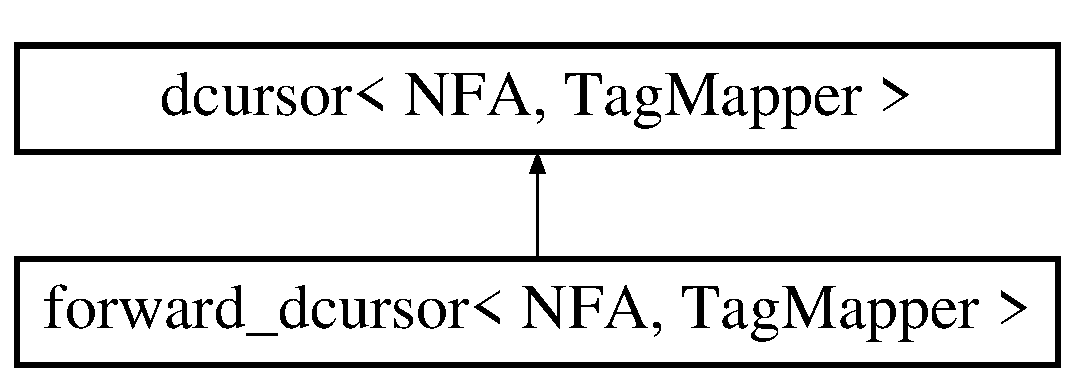
\includegraphics[height=2.000000cm]{classastl_1_1dcursor}
\end{center}
\end{figure}


\subsection{Detailed Description}
\subsubsection*{template$<$typename N\+F\+A, typename Tag\+Mapper = default\+\_\+tag\+\_\+mapper$<$\+N\+F\+A$>$$>$class astl\+::dcursor$<$ N\+F\+A, Tag\+Mapper $>$}

A plain cursor to a non-\/deterministic automaton computing the determinization on-\/the-\/fly. 

\begin{DoxyParagraph}{Associated Helper Functions}
\#plaindc() 
\end{DoxyParagraph}

\section{D\+F\+A\+\_\+base$<$ Char\+Traits, Tag\+Type, State\+Data\+\_\+, State\+Type $>$ Class Template Reference}
\label{classastl_1_1DFA__base}\index{D\+F\+A\+\_\+base$<$ Char\+Traits, Tag\+Type, State\+Data\+\_\+, State\+Type $>$@{D\+F\+A\+\_\+base$<$ Char\+Traits, Tag\+Type, State\+Data\+\_\+, State\+Type $>$}}


Base class for A\+S\+T\+L deterministic automaton containers.  




{\ttfamily \#include $<$dfa\+\_\+base.\+h$>$}



Inherits D\+F\+A\+\_\+concept.

\subsection*{Public Types}
\begin{DoxyCompactItemize}
\item 
typedef Char\+Traits {\bf char\+\_\+traits}\label{classastl_1_1DFA__base_a7f7f29ddd3e8db5ce7820504bd30fdb9}

\begin{DoxyCompactList}\small\item\em Character traits describing \doxyref{char\+\_\+type}{p.}{classastl_1_1DFA__base_a5cf5887889a6276ff07d3101391a63a3}. \end{DoxyCompactList}\item 
typedef Char\+Traits\+::char\+\_\+type {\bf char\+\_\+type}\label{classastl_1_1DFA__base_a5cf5887889a6276ff07d3101391a63a3}

\begin{DoxyCompactList}\small\item\em The type of the transitions letters. \end{DoxyCompactList}\item 
typedef State\+Type {\bf state\+\_\+type}\label{classastl_1_1DFA__base_a133508bf1c8112d5cace97e216c278a2}

\begin{DoxyCompactList}\small\item\em The type of the automaton-\/states identifiers. \end{DoxyCompactList}\item 
typedef Tag\+Type {\bf tag\+\_\+type}\label{classastl_1_1DFA__base_a3c40b9376fa70e2df00a1938cc425082}

\begin{DoxyCompactList}\small\item\em The type of the data attached to states. \end{DoxyCompactList}\end{DoxyCompactItemize}
\subsection*{Public Member Functions}
\begin{DoxyCompactItemize}
\item 
const\+\_\+iterator {\bf begin} () const 
\item 
void {\bf copy\+\_\+state} ({\bf state\+\_\+type} from, {\bf state\+\_\+type} to)
\begin{DoxyCompactList}\small\item\em Makes the state {\ttfamily to} an exact copy of the state {\ttfamily from}. \end{DoxyCompactList}\item 
void {\bf del\+\_\+state} ({\bf state\+\_\+type} s)
\begin{DoxyCompactList}\small\item\em Destroyes the state {\ttfamily s}. \end{DoxyCompactList}\item 
{\bf state\+\_\+type} {\bf duplicate\+\_\+state} ({\bf state\+\_\+type} q)
\begin{DoxyCompactList}\small\item\em Allocates an exact copy of the state {\ttfamily q}. \end{DoxyCompactList}\item 
const\+\_\+iterator {\bf end} () const 
\item 
bool {\bf final} ({\bf state\+\_\+type} s) const 
\item 
char \& {\bf final} ({\bf state\+\_\+type} s)
\item 
void {\bf initial} ({\bf state\+\_\+type} s)
\begin{DoxyCompactList}\small\item\em Sets the initial state of the automaton to {\ttfamily s}. \end{DoxyCompactList}\item 
{\bf state\+\_\+type} {\bf initial} () const 
\item 
{\bf state\+\_\+type} {\bf new\+\_\+state} ()
\begin{DoxyCompactList}\small\item\em Allocates a new state structure. \end{DoxyCompactList}\item 
unsigned long {\bf state\+\_\+count} () const 
\item 
{\bf tag\+\_\+type} \& {\bf tag} ({\bf state\+\_\+type} s)
\item 
const {\bf tag\+\_\+type} \& {\bf tag} ({\bf state\+\_\+type} s) const 
\item 
unsigned long {\bf trans\+\_\+count} () const 
\end{DoxyCompactItemize}


\subsection{Detailed Description}
\subsubsection*{template$<$class Char\+Traits, class Tag\+Type, class State\+Data\+\_\+, class State\+Type = unsigned int$>$class astl\+::\+D\+F\+A\+\_\+base$<$ Char\+Traits, Tag\+Type, State\+Data\+\_\+, State\+Type $>$}

Base class for A\+S\+T\+L deterministic automaton containers. 

It takes care of common functionalities dealing with states allocation/deallocation. 

\subsection{Member Function Documentation}
\index{astl\+::\+D\+F\+A\+\_\+base@{astl\+::\+D\+F\+A\+\_\+base}!begin@{begin}}
\index{begin@{begin}!astl\+::\+D\+F\+A\+\_\+base@{astl\+::\+D\+F\+A\+\_\+base}}
\subsubsection[{begin}]{\setlength{\rightskip}{0pt plus 5cm}const\+\_\+iterator begin (
\begin{DoxyParamCaption}
{}
\end{DoxyParamCaption}
) const}\label{classastl_1_1DFA__base_aa4b02d4f1a8500fb07a551069060709f}
\begin{DoxyReturn}{Returns}
a forward iterator on the beginning of the sequence of the automaton states of type {\ttfamily state\+\_\+type} arranged in an undefined order (probably in allocation order but that is not a requirement). 
\end{DoxyReturn}
\index{astl\+::\+D\+F\+A\+\_\+base@{astl\+::\+D\+F\+A\+\_\+base}!copy\+\_\+state@{copy\+\_\+state}}
\index{copy\+\_\+state@{copy\+\_\+state}!astl\+::\+D\+F\+A\+\_\+base@{astl\+::\+D\+F\+A\+\_\+base}}
\subsubsection[{copy\+\_\+state}]{\setlength{\rightskip}{0pt plus 5cm}void copy\+\_\+state (
\begin{DoxyParamCaption}
\item[{{\bf state\+\_\+type}}]{from, }
\item[{{\bf state\+\_\+type}}]{to}
\end{DoxyParamCaption}
)}\label{classastl_1_1DFA__base_a4e3e0654b66dfe88b0a093de04437bec}


Makes the state {\ttfamily to} an exact copy of the state {\ttfamily from}. 

The tag and the transitions of {\ttfamily to} are destroyed and the new ones are copy-\/constructed from those of {\ttfamily from}. \begin{DoxyPrecond}{Precondition}
{\ttfamily from} has been returned by a previous call to {\ttfamily \doxyref{new\+\_\+state()}{p.}{classastl_1_1DFA__base_a252db8b50da681bd88660c6f1166f6c7}} 

{\ttfamily to} has been returned by a previous call to {\ttfamily \doxyref{new\+\_\+state()}{p.}{classastl_1_1DFA__base_a252db8b50da681bd88660c6f1166f6c7}} 
\end{DoxyPrecond}
\index{astl\+::\+D\+F\+A\+\_\+base@{astl\+::\+D\+F\+A\+\_\+base}!del\+\_\+state@{del\+\_\+state}}
\index{del\+\_\+state@{del\+\_\+state}!astl\+::\+D\+F\+A\+\_\+base@{astl\+::\+D\+F\+A\+\_\+base}}
\subsubsection[{del\+\_\+state}]{\setlength{\rightskip}{0pt plus 5cm}void del\+\_\+state (
\begin{DoxyParamCaption}
\item[{{\bf state\+\_\+type}}]{s}
\end{DoxyParamCaption}
)}\label{classastl_1_1DFA__base_a8bf68bf8c77e67ebfca27a8472e4c913}


Destroyes the state {\ttfamily s}. 

The tag and the transitions are destroyed. \begin{DoxyPrecond}{Precondition}
{\ttfamily s} has been returned by a previous call to {\ttfamily \doxyref{new\+\_\+state()}{p.}{classastl_1_1DFA__base_a252db8b50da681bd88660c6f1166f6c7}} 
\end{DoxyPrecond}
\index{astl\+::\+D\+F\+A\+\_\+base@{astl\+::\+D\+F\+A\+\_\+base}!duplicate\+\_\+state@{duplicate\+\_\+state}}
\index{duplicate\+\_\+state@{duplicate\+\_\+state}!astl\+::\+D\+F\+A\+\_\+base@{astl\+::\+D\+F\+A\+\_\+base}}
\subsubsection[{duplicate\+\_\+state}]{\setlength{\rightskip}{0pt plus 5cm}{\bf state\+\_\+type} duplicate\+\_\+state (
\begin{DoxyParamCaption}
\item[{{\bf state\+\_\+type}}]{q}
\end{DoxyParamCaption}
)}\label{classastl_1_1DFA__base_a4788aa4f6e09d5b70bc2f3defabb1ea7}


Allocates an exact copy of the state {\ttfamily q}. 

\begin{DoxyReturn}{Returns}
the id of the freshly allocated state 
\end{DoxyReturn}
\begin{DoxyPrecond}{Precondition}
{\ttfamily q} has been returned by a previous call to {\ttfamily \doxyref{new\+\_\+state()}{p.}{classastl_1_1DFA__base_a252db8b50da681bd88660c6f1166f6c7}} 
\end{DoxyPrecond}
\index{astl\+::\+D\+F\+A\+\_\+base@{astl\+::\+D\+F\+A\+\_\+base}!end@{end}}
\index{end@{end}!astl\+::\+D\+F\+A\+\_\+base@{astl\+::\+D\+F\+A\+\_\+base}}
\subsubsection[{end}]{\setlength{\rightskip}{0pt plus 5cm}const\+\_\+iterator end (
\begin{DoxyParamCaption}
{}
\end{DoxyParamCaption}
) const}\label{classastl_1_1DFA__base_a350132543d80a1c1e5be844e6d2878ea}
\begin{DoxyReturn}{Returns}
a past-\/the-\/end forward iterator on the sequence of the automaton states. 
\end{DoxyReturn}
\index{astl\+::\+D\+F\+A\+\_\+base@{astl\+::\+D\+F\+A\+\_\+base}!final@{final}}
\index{final@{final}!astl\+::\+D\+F\+A\+\_\+base@{astl\+::\+D\+F\+A\+\_\+base}}
\subsubsection[{final}]{\setlength{\rightskip}{0pt plus 5cm}bool final (
\begin{DoxyParamCaption}
\item[{{\bf state\+\_\+type}}]{s}
\end{DoxyParamCaption}
) const}\label{classastl_1_1DFA__base_ad1882121c53bdedd74df649d71b70a4c}
\begin{DoxyReturn}{Returns}
{\ttfamily true} if {\ttfamily s} is a final state. 
\end{DoxyReturn}
\begin{DoxyPrecond}{Precondition}
{\ttfamily s} has been returned by a previous call to {\ttfamily \doxyref{new\+\_\+state()}{p.}{classastl_1_1DFA__base_a252db8b50da681bd88660c6f1166f6c7}} 
\end{DoxyPrecond}
\index{astl\+::\+D\+F\+A\+\_\+base@{astl\+::\+D\+F\+A\+\_\+base}!final@{final}}
\index{final@{final}!astl\+::\+D\+F\+A\+\_\+base@{astl\+::\+D\+F\+A\+\_\+base}}
\subsubsection[{final}]{\setlength{\rightskip}{0pt plus 5cm}char\& final (
\begin{DoxyParamCaption}
\item[{{\bf state\+\_\+type}}]{s}
\end{DoxyParamCaption}
)}\label{classastl_1_1DFA__base_a8011bf53b33ceac2c71ca364bbb1fbc3}
\begin{DoxyReturn}{Returns}
a reference to a boolean that, if assigned {\ttfamily true} sets the state {\ttfamily s} to be a final state and if assigned {\ttfamily false} sets {\ttfamily s} to be a non-\/final state. 
\end{DoxyReturn}
\begin{DoxyPrecond}{Precondition}
{\ttfamily s} has been returned by a previous call to {\ttfamily \doxyref{new\+\_\+state()}{p.}{classastl_1_1DFA__base_a252db8b50da681bd88660c6f1166f6c7}} 
\end{DoxyPrecond}
\index{astl\+::\+D\+F\+A\+\_\+base@{astl\+::\+D\+F\+A\+\_\+base}!initial@{initial}}
\index{initial@{initial}!astl\+::\+D\+F\+A\+\_\+base@{astl\+::\+D\+F\+A\+\_\+base}}
\subsubsection[{initial}]{\setlength{\rightskip}{0pt plus 5cm}void initial (
\begin{DoxyParamCaption}
\item[{{\bf state\+\_\+type}}]{s}
\end{DoxyParamCaption}
)}\label{classastl_1_1DFA__base_a0512d51289bf8ed1a0d42df6272c0d70}


Sets the initial state of the automaton to {\ttfamily s}. 

\begin{DoxyPrecond}{Precondition}
{\ttfamily s} has been returned by a previous call to {\ttfamily \doxyref{new\+\_\+state()}{p.}{classastl_1_1DFA__base_a252db8b50da681bd88660c6f1166f6c7}} 
\end{DoxyPrecond}
\begin{DoxyPostcond}{Postcondition}

\begin{DoxyCode}
initial() == s 
\end{DoxyCode}
 
\end{DoxyPostcond}
\index{astl\+::\+D\+F\+A\+\_\+base@{astl\+::\+D\+F\+A\+\_\+base}!initial@{initial}}
\index{initial@{initial}!astl\+::\+D\+F\+A\+\_\+base@{astl\+::\+D\+F\+A\+\_\+base}}
\subsubsection[{initial}]{\setlength{\rightskip}{0pt plus 5cm}{\bf state\+\_\+type} initial (
\begin{DoxyParamCaption}
{}
\end{DoxyParamCaption}
) const}\label{classastl_1_1DFA__base_a4edaf60fafcacf017837f0a5eb5bc39b}
\begin{DoxyReturn}{Returns}
the initial state of the automaton. 
\end{DoxyReturn}


Referenced by D\+F\+A\+\_\+base$<$ Char\+Traits, Tag, matrix\+\_\+line$<$ Char\+Traits, unsigned short $>$, unsigned short $>$\+::del\+\_\+state().

\index{astl\+::\+D\+F\+A\+\_\+base@{astl\+::\+D\+F\+A\+\_\+base}!new\+\_\+state@{new\+\_\+state}}
\index{new\+\_\+state@{new\+\_\+state}!astl\+::\+D\+F\+A\+\_\+base@{astl\+::\+D\+F\+A\+\_\+base}}
\subsubsection[{new\+\_\+state}]{\setlength{\rightskip}{0pt plus 5cm}{\bf state\+\_\+type} new\+\_\+state (
\begin{DoxyParamCaption}
{}
\end{DoxyParamCaption}
)}\label{classastl_1_1DFA__base_a252db8b50da681bd88660c6f1166f6c7}


Allocates a new state structure. 

The newly created state is non-\/final and has no transitions. The tag is default-\/constructed. \begin{DoxyReturn}{Returns}
the id of the freshly allocated state 
\end{DoxyReturn}
\index{astl\+::\+D\+F\+A\+\_\+base@{astl\+::\+D\+F\+A\+\_\+base}!state\+\_\+count@{state\+\_\+count}}
\index{state\+\_\+count@{state\+\_\+count}!astl\+::\+D\+F\+A\+\_\+base@{astl\+::\+D\+F\+A\+\_\+base}}
\subsubsection[{state\+\_\+count}]{\setlength{\rightskip}{0pt plus 5cm}unsigned long state\+\_\+count (
\begin{DoxyParamCaption}
{}
\end{DoxyParamCaption}
) const}\label{classastl_1_1DFA__base_abbd3928d673458d0fa63e568a950a83d}
\begin{DoxyReturn}{Returns}
the number of states in the automaton 
\end{DoxyReturn}
\index{astl\+::\+D\+F\+A\+\_\+base@{astl\+::\+D\+F\+A\+\_\+base}!tag@{tag}}
\index{tag@{tag}!astl\+::\+D\+F\+A\+\_\+base@{astl\+::\+D\+F\+A\+\_\+base}}
\subsubsection[{tag}]{\setlength{\rightskip}{0pt plus 5cm}{\bf tag\+\_\+type}\& tag (
\begin{DoxyParamCaption}
\item[{{\bf state\+\_\+type}}]{s}
\end{DoxyParamCaption}
)}\label{classastl_1_1DFA__base_a3dd4257038bc77fa1cc7d9bf0afc29d5}
\begin{DoxyReturn}{Returns}
the data attached to the state {\ttfamily s} 
\end{DoxyReturn}
\begin{DoxyPrecond}{Precondition}
{\ttfamily s} has been returned by a previous call to {\ttfamily \doxyref{new\+\_\+state()}{p.}{classastl_1_1DFA__base_a252db8b50da681bd88660c6f1166f6c7}} 
\end{DoxyPrecond}
\index{astl\+::\+D\+F\+A\+\_\+base@{astl\+::\+D\+F\+A\+\_\+base}!tag@{tag}}
\index{tag@{tag}!astl\+::\+D\+F\+A\+\_\+base@{astl\+::\+D\+F\+A\+\_\+base}}
\subsubsection[{tag}]{\setlength{\rightskip}{0pt plus 5cm}const {\bf tag\+\_\+type}\& tag (
\begin{DoxyParamCaption}
\item[{{\bf state\+\_\+type}}]{s}
\end{DoxyParamCaption}
) const}\label{classastl_1_1DFA__base_aae6988f0a4fda8a527b52781ab9f0d59}
\begin{DoxyReturn}{Returns}
the data attached to the state {\ttfamily s} 
\end{DoxyReturn}
\begin{DoxyPrecond}{Precondition}
{\ttfamily s} has been returned by a previous call to {\ttfamily \doxyref{new\+\_\+state()}{p.}{classastl_1_1DFA__base_a252db8b50da681bd88660c6f1166f6c7}} 
\end{DoxyPrecond}
\index{astl\+::\+D\+F\+A\+\_\+base@{astl\+::\+D\+F\+A\+\_\+base}!trans\+\_\+count@{trans\+\_\+count}}
\index{trans\+\_\+count@{trans\+\_\+count}!astl\+::\+D\+F\+A\+\_\+base@{astl\+::\+D\+F\+A\+\_\+base}}
\subsubsection[{trans\+\_\+count}]{\setlength{\rightskip}{0pt plus 5cm}unsigned long trans\+\_\+count (
\begin{DoxyParamCaption}
{}
\end{DoxyParamCaption}
) const}\label{classastl_1_1DFA__base_a3f2590089bd23eb738c72bf9acfb9c44}
\begin{DoxyReturn}{Returns}
the number of transitions in the automaton 
\end{DoxyReturn}

\section{D\+F\+A\+\_\+bin$<$ Sigma\+\_\+, Tag\+\_\+ $>$ Class Template Reference}
\label{classastl_1_1DFA__bin}\index{D\+F\+A\+\_\+bin$<$ Sigma\+\_\+, Tag\+\_\+ $>$@{D\+F\+A\+\_\+bin$<$ Sigma\+\_\+, Tag\+\_\+ $>$}}


A deterministic automaton container class that stores the transition of a state in a standard sorted {\ttfamily vector} of pairs of letters and transitions targets.  




{\ttfamily \#include $<$dfa\+\_\+bin.\+h$>$}

Inheritance diagram for D\+F\+A\+\_\+bin$<$ Sigma\+\_\+, Tag\+\_\+ $>$\+:\begin{figure}[H]
\begin{center}
\leavevmode
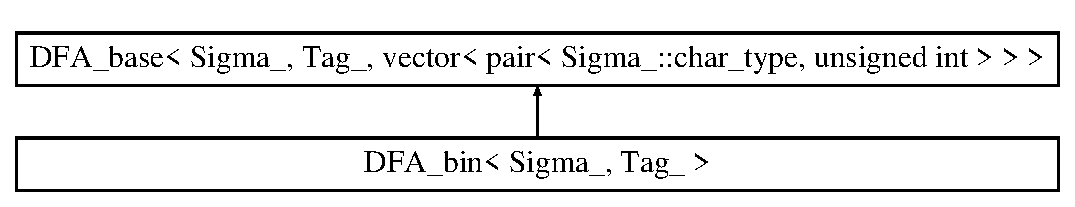
\includegraphics[height=2.000000cm]{classastl_1_1DFA__bin}
\end{center}
\end{figure}
\subsection*{Public Member Functions}
\begin{DoxyCompactItemize}
\item 
const\+\_\+iterator {\bf begin} () const
\item 
void {\bf copy\+\_\+state} (state\+\_\+type from, state\+\_\+type to)
\begin{DoxyCompactList}\small\item\em Makes the state {\ttfamily to} an exact copy of the state {\ttfamily from}. \end{DoxyCompactList}\item 
void {\bf del\+\_\+state} (state\+\_\+type s)
\begin{DoxyCompactList}\small\item\em Destroyes the state {\ttfamily s}. \end{DoxyCompactList}\item 
state\+\_\+type {\bf duplicate\+\_\+state} (state\+\_\+type q)
\begin{DoxyCompactList}\small\item\em Allocates an exact copy of the state {\ttfamily q}. \end{DoxyCompactList}\item 
const\+\_\+iterator {\bf end} () const
\item 
bool {\bf final} (state\+\_\+type s) const
\item 
char \& {\bf final} (state\+\_\+type s)
\item 
void {\bf initial} (state\+\_\+type s)
\begin{DoxyCompactList}\small\item\em Sets the initial state of the automaton to {\ttfamily s}. \end{DoxyCompactList}\item 
state\+\_\+type {\bf initial} () const
\item 
state\+\_\+type {\bf new\+\_\+state} ()
\begin{DoxyCompactList}\small\item\em Allocates a new state structure. \end{DoxyCompactList}\item 
unsigned long {\bf state\+\_\+count} () const
\item 
tag\+\_\+type \& {\bf tag} (state\+\_\+type s)
\item 
const tag\+\_\+type \& {\bf tag} (state\+\_\+type s) const
\item 
unsigned long {\bf trans\+\_\+count} () const
\end{DoxyCompactItemize}


\subsection{Detailed Description}
\subsubsection*{template$<$class Sigma\+\_\+ = plain, class Tag\+\_\+ = empty\+\_\+tag$>$class astl\+::\+D\+F\+A\+\_\+bin$<$ Sigma\+\_\+, Tag\+\_\+ $>$}

A deterministic automaton container class that stores the transition of a state in a standard sorted {\ttfamily vector} of pairs of letters and transitions targets. 

Access is in logarithmic time through a binary search but insertion and deletion are in linear time.

It is the best when it comes to depth-\/ and breadth-\/first traversals and when saving memory space is important but is slow at building and maintaining.

The ordering used for sorting the transition uses the one defined by the character traits {\ttfamily Char\+Traits\+::lt()}.

\begin{DoxyParagraph}{Template parameters}
\begin{TabularC}{4}
\hline
\rowcolor{lightgray}{\bf Parameter}&{\bf Description}&{\bf Default}&{\bf Requirements }\\\cline{1-4}
{\ttfamily Char\+Traits} &Character traits describing the letters that the transitions bear.&{\ttfamily plain} &{\ttfamily Char\+Traits} is a model of \#\+Alphabet \\\cline{1-4}
{\ttfamily Tag} &The type of the data attached to states.&{\ttfamily empty\+\_\+tag} &\\\cline{1-4}
\end{TabularC}

\end{DoxyParagraph}


\subsection{Member Function Documentation}
\index{astl\+::\+D\+F\+A\+\_\+bin@{astl\+::\+D\+F\+A\+\_\+bin}!begin@{begin}}
\index{begin@{begin}!astl\+::\+D\+F\+A\+\_\+bin@{astl\+::\+D\+F\+A\+\_\+bin}}
\subsubsection[{begin}]{\setlength{\rightskip}{0pt plus 5cm}const\+\_\+iterator begin (
\begin{DoxyParamCaption}
{}
\end{DoxyParamCaption}
) const\hspace{0.3cm}{\ttfamily [inherited]}}\label{classastl_1_1DFA__base_aa4b02d4f1a8500fb07a551069060709f}
\begin{DoxyReturn}{Returns}
a forward iterator on the beginning of the sequence of the automaton states of type {\ttfamily state\+\_\+type} arranged in an undefined order (probably in allocation order but that is not a requirement). 
\end{DoxyReturn}
\index{astl\+::\+D\+F\+A\+\_\+bin@{astl\+::\+D\+F\+A\+\_\+bin}!copy\+\_\+state@{copy\+\_\+state}}
\index{copy\+\_\+state@{copy\+\_\+state}!astl\+::\+D\+F\+A\+\_\+bin@{astl\+::\+D\+F\+A\+\_\+bin}}
\subsubsection[{copy\+\_\+state}]{\setlength{\rightskip}{0pt plus 5cm}void copy\+\_\+state (
\begin{DoxyParamCaption}
\item[{{\bf state\+\_\+type}}]{from, }
\item[{{\bf state\+\_\+type}}]{to}
\end{DoxyParamCaption}
)\hspace{0.3cm}{\ttfamily [inherited]}}\label{classastl_1_1DFA__base_a4e3e0654b66dfe88b0a093de04437bec}


Makes the state {\ttfamily to} an exact copy of the state {\ttfamily from}. 

The tag and the transitions of {\ttfamily to} are destroyed and the new ones are copy-\/constructed from those of {\ttfamily from}. \begin{DoxyPrecond}{Precondition}
{\ttfamily from} has been returned by a previous call to {\ttfamily \doxyref{new\+\_\+state()}{p.}{classastl_1_1DFA__base_a252db8b50da681bd88660c6f1166f6c7}} 

{\ttfamily to} has been returned by a previous call to {\ttfamily \doxyref{new\+\_\+state()}{p.}{classastl_1_1DFA__base_a252db8b50da681bd88660c6f1166f6c7}} 
\end{DoxyPrecond}
\index{astl\+::\+D\+F\+A\+\_\+bin@{astl\+::\+D\+F\+A\+\_\+bin}!del\+\_\+state@{del\+\_\+state}}
\index{del\+\_\+state@{del\+\_\+state}!astl\+::\+D\+F\+A\+\_\+bin@{astl\+::\+D\+F\+A\+\_\+bin}}
\subsubsection[{del\+\_\+state}]{\setlength{\rightskip}{0pt plus 5cm}void del\+\_\+state (
\begin{DoxyParamCaption}
\item[{{\bf state\+\_\+type}}]{s}
\end{DoxyParamCaption}
)\hspace{0.3cm}{\ttfamily [inherited]}}\label{classastl_1_1DFA__base_a8bf68bf8c77e67ebfca27a8472e4c913}


Destroyes the state {\ttfamily s}. 

The tag and the transitions are destroyed. \begin{DoxyPrecond}{Precondition}
{\ttfamily s} has been returned by a previous call to {\ttfamily \doxyref{new\+\_\+state()}{p.}{classastl_1_1DFA__base_a252db8b50da681bd88660c6f1166f6c7}} 
\end{DoxyPrecond}
\index{astl\+::\+D\+F\+A\+\_\+bin@{astl\+::\+D\+F\+A\+\_\+bin}!duplicate\+\_\+state@{duplicate\+\_\+state}}
\index{duplicate\+\_\+state@{duplicate\+\_\+state}!astl\+::\+D\+F\+A\+\_\+bin@{astl\+::\+D\+F\+A\+\_\+bin}}
\subsubsection[{duplicate\+\_\+state}]{\setlength{\rightskip}{0pt plus 5cm}state\+\_\+type duplicate\+\_\+state (
\begin{DoxyParamCaption}
\item[{{\bf state\+\_\+type}}]{q}
\end{DoxyParamCaption}
)\hspace{0.3cm}{\ttfamily [inherited]}}\label{classastl_1_1DFA__base_a4788aa4f6e09d5b70bc2f3defabb1ea7}


Allocates an exact copy of the state {\ttfamily q}. 

\begin{DoxyReturn}{Returns}
the id of the freshly allocated state 
\end{DoxyReturn}
\begin{DoxyPrecond}{Precondition}
{\ttfamily q} has been returned by a previous call to {\ttfamily \doxyref{new\+\_\+state()}{p.}{classastl_1_1DFA__base_a252db8b50da681bd88660c6f1166f6c7}} 
\end{DoxyPrecond}
\index{astl\+::\+D\+F\+A\+\_\+bin@{astl\+::\+D\+F\+A\+\_\+bin}!end@{end}}
\index{end@{end}!astl\+::\+D\+F\+A\+\_\+bin@{astl\+::\+D\+F\+A\+\_\+bin}}
\subsubsection[{end}]{\setlength{\rightskip}{0pt plus 5cm}const\+\_\+iterator end (
\begin{DoxyParamCaption}
{}
\end{DoxyParamCaption}
) const\hspace{0.3cm}{\ttfamily [inherited]}}\label{classastl_1_1DFA__base_a350132543d80a1c1e5be844e6d2878ea}
\begin{DoxyReturn}{Returns}
a past-\/the-\/end forward iterator on the sequence of the automaton states. 
\end{DoxyReturn}
\index{astl\+::\+D\+F\+A\+\_\+bin@{astl\+::\+D\+F\+A\+\_\+bin}!final@{final}}
\index{final@{final}!astl\+::\+D\+F\+A\+\_\+bin@{astl\+::\+D\+F\+A\+\_\+bin}}
\subsubsection[{final}]{\setlength{\rightskip}{0pt plus 5cm}bool final (
\begin{DoxyParamCaption}
\item[{{\bf state\+\_\+type}}]{s}
\end{DoxyParamCaption}
) const\hspace{0.3cm}{\ttfamily [inherited]}}\label{classastl_1_1DFA__base_ad1882121c53bdedd74df649d71b70a4c}
\begin{DoxyReturn}{Returns}
{\ttfamily true} if {\ttfamily s} is a final state. 
\end{DoxyReturn}
\begin{DoxyPrecond}{Precondition}
{\ttfamily s} has been returned by a previous call to {\ttfamily \doxyref{new\+\_\+state()}{p.}{classastl_1_1DFA__base_a252db8b50da681bd88660c6f1166f6c7}} 
\end{DoxyPrecond}
\index{astl\+::\+D\+F\+A\+\_\+bin@{astl\+::\+D\+F\+A\+\_\+bin}!final@{final}}
\index{final@{final}!astl\+::\+D\+F\+A\+\_\+bin@{astl\+::\+D\+F\+A\+\_\+bin}}
\subsubsection[{final}]{\setlength{\rightskip}{0pt plus 5cm}char\& final (
\begin{DoxyParamCaption}
\item[{{\bf state\+\_\+type}}]{s}
\end{DoxyParamCaption}
)\hspace{0.3cm}{\ttfamily [inherited]}}\label{classastl_1_1DFA__base_a8011bf53b33ceac2c71ca364bbb1fbc3}
\begin{DoxyReturn}{Returns}
a reference to a boolean that, if assigned {\ttfamily true} sets the state {\ttfamily s} to be a final state and if assigned {\ttfamily false} sets {\ttfamily s} to be a non-\/final state. 
\end{DoxyReturn}
\begin{DoxyPrecond}{Precondition}
{\ttfamily s} has been returned by a previous call to {\ttfamily \doxyref{new\+\_\+state()}{p.}{classastl_1_1DFA__base_a252db8b50da681bd88660c6f1166f6c7}} 
\end{DoxyPrecond}
\index{astl\+::\+D\+F\+A\+\_\+bin@{astl\+::\+D\+F\+A\+\_\+bin}!initial@{initial}}
\index{initial@{initial}!astl\+::\+D\+F\+A\+\_\+bin@{astl\+::\+D\+F\+A\+\_\+bin}}
\subsubsection[{initial}]{\setlength{\rightskip}{0pt plus 5cm}void initial (
\begin{DoxyParamCaption}
\item[{{\bf state\+\_\+type}}]{s}
\end{DoxyParamCaption}
)\hspace{0.3cm}{\ttfamily [inherited]}}\label{classastl_1_1DFA__base_a0512d51289bf8ed1a0d42df6272c0d70}


Sets the initial state of the automaton to {\ttfamily s}. 

\begin{DoxyPrecond}{Precondition}
{\ttfamily s} has been returned by a previous call to {\ttfamily \doxyref{new\+\_\+state()}{p.}{classastl_1_1DFA__base_a252db8b50da681bd88660c6f1166f6c7}} 
\end{DoxyPrecond}
\begin{DoxyPostcond}{Postcondition}

\begin{DoxyCode}
initial() == s 
\end{DoxyCode}
 
\end{DoxyPostcond}
\index{astl\+::\+D\+F\+A\+\_\+bin@{astl\+::\+D\+F\+A\+\_\+bin}!initial@{initial}}
\index{initial@{initial}!astl\+::\+D\+F\+A\+\_\+bin@{astl\+::\+D\+F\+A\+\_\+bin}}
\subsubsection[{initial}]{\setlength{\rightskip}{0pt plus 5cm}state\+\_\+type initial (
\begin{DoxyParamCaption}
{}
\end{DoxyParamCaption}
) const\hspace{0.3cm}{\ttfamily [inherited]}}\label{classastl_1_1DFA__base_a4edaf60fafcacf017837f0a5eb5bc39b}
\begin{DoxyReturn}{Returns}
the initial state of the automaton. 
\end{DoxyReturn}
\index{astl\+::\+D\+F\+A\+\_\+bin@{astl\+::\+D\+F\+A\+\_\+bin}!new\+\_\+state@{new\+\_\+state}}
\index{new\+\_\+state@{new\+\_\+state}!astl\+::\+D\+F\+A\+\_\+bin@{astl\+::\+D\+F\+A\+\_\+bin}}
\subsubsection[{new\+\_\+state}]{\setlength{\rightskip}{0pt plus 5cm}state\+\_\+type new\+\_\+state (
\begin{DoxyParamCaption}
{}
\end{DoxyParamCaption}
)\hspace{0.3cm}{\ttfamily [inherited]}}\label{classastl_1_1DFA__base_a252db8b50da681bd88660c6f1166f6c7}


Allocates a new state structure. 

The newly created state is non-\/final and has no transitions. The tag is default-\/constructed. \begin{DoxyReturn}{Returns}
the id of the freshly allocated state 
\end{DoxyReturn}
\index{astl\+::\+D\+F\+A\+\_\+bin@{astl\+::\+D\+F\+A\+\_\+bin}!state\+\_\+count@{state\+\_\+count}}
\index{state\+\_\+count@{state\+\_\+count}!astl\+::\+D\+F\+A\+\_\+bin@{astl\+::\+D\+F\+A\+\_\+bin}}
\subsubsection[{state\+\_\+count}]{\setlength{\rightskip}{0pt plus 5cm}unsigned long state\+\_\+count (
\begin{DoxyParamCaption}
{}
\end{DoxyParamCaption}
) const\hspace{0.3cm}{\ttfamily [inherited]}}\label{classastl_1_1DFA__base_abbd3928d673458d0fa63e568a950a83d}
\begin{DoxyReturn}{Returns}
the number of states in the automaton 
\end{DoxyReturn}
\index{astl\+::\+D\+F\+A\+\_\+bin@{astl\+::\+D\+F\+A\+\_\+bin}!tag@{tag}}
\index{tag@{tag}!astl\+::\+D\+F\+A\+\_\+bin@{astl\+::\+D\+F\+A\+\_\+bin}}
\subsubsection[{tag}]{\setlength{\rightskip}{0pt plus 5cm}tag\+\_\+type\& tag (
\begin{DoxyParamCaption}
\item[{{\bf state\+\_\+type}}]{s}
\end{DoxyParamCaption}
)\hspace{0.3cm}{\ttfamily [inherited]}}\label{classastl_1_1DFA__base_a3dd4257038bc77fa1cc7d9bf0afc29d5}
\begin{DoxyReturn}{Returns}
the data attached to the state {\ttfamily s} 
\end{DoxyReturn}
\begin{DoxyPrecond}{Precondition}
{\ttfamily s} has been returned by a previous call to {\ttfamily \doxyref{new\+\_\+state()}{p.}{classastl_1_1DFA__base_a252db8b50da681bd88660c6f1166f6c7}} 
\end{DoxyPrecond}
\index{astl\+::\+D\+F\+A\+\_\+bin@{astl\+::\+D\+F\+A\+\_\+bin}!tag@{tag}}
\index{tag@{tag}!astl\+::\+D\+F\+A\+\_\+bin@{astl\+::\+D\+F\+A\+\_\+bin}}
\subsubsection[{tag}]{\setlength{\rightskip}{0pt plus 5cm}const tag\+\_\+type\& tag (
\begin{DoxyParamCaption}
\item[{{\bf state\+\_\+type}}]{s}
\end{DoxyParamCaption}
) const\hspace{0.3cm}{\ttfamily [inherited]}}\label{classastl_1_1DFA__base_aae6988f0a4fda8a527b52781ab9f0d59}
\begin{DoxyReturn}{Returns}
the data attached to the state {\ttfamily s} 
\end{DoxyReturn}
\begin{DoxyPrecond}{Precondition}
{\ttfamily s} has been returned by a previous call to {\ttfamily \doxyref{new\+\_\+state()}{p.}{classastl_1_1DFA__base_a252db8b50da681bd88660c6f1166f6c7}} 
\end{DoxyPrecond}
\index{astl\+::\+D\+F\+A\+\_\+bin@{astl\+::\+D\+F\+A\+\_\+bin}!trans\+\_\+count@{trans\+\_\+count}}
\index{trans\+\_\+count@{trans\+\_\+count}!astl\+::\+D\+F\+A\+\_\+bin@{astl\+::\+D\+F\+A\+\_\+bin}}
\subsubsection[{trans\+\_\+count}]{\setlength{\rightskip}{0pt plus 5cm}unsigned long trans\+\_\+count (
\begin{DoxyParamCaption}
{}
\end{DoxyParamCaption}
) const\hspace{0.3cm}{\ttfamily [inherited]}}\label{classastl_1_1DFA__base_a3f2590089bd23eb738c72bf9acfb9c44}
\begin{DoxyReturn}{Returns}
the number of transitions in the automaton 
\end{DoxyReturn}

\section{D\+F\+A\+\_\+map$<$ Char\+Traits, Tag $>$ Class Template Reference}
\label{classastl_1_1DFA__map}\index{D\+F\+A\+\_\+map$<$ Char\+Traits, Tag $>$@{D\+F\+A\+\_\+map$<$ Char\+Traits, Tag $>$}}


A deterministic automaton container class that stores the transition of a state in a standard {\ttfamily map} associating letters to transitions targets.  




{\ttfamily \#include $<$dfa\+\_\+map.\+h$>$}

Inheritance diagram for D\+F\+A\+\_\+map$<$ Char\+Traits, Tag $>$\+:\begin{figure}[H]
\begin{center}
\leavevmode
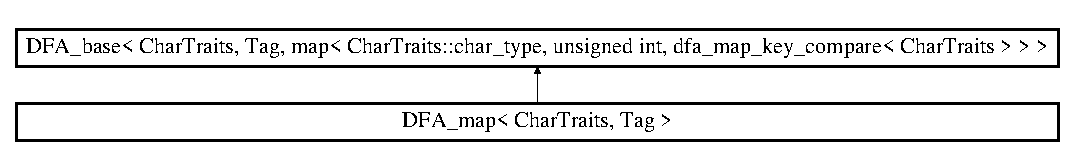
\includegraphics[height=1.666667cm]{classastl_1_1DFA__map}
\end{center}
\end{figure}
\subsection*{Public Member Functions}
\begin{DoxyCompactItemize}
\item 
const\+\_\+iterator {\bf begin} () const
\item 
void {\bf copy\+\_\+state} (state\+\_\+type from, state\+\_\+type to)
\begin{DoxyCompactList}\small\item\em Makes the state {\ttfamily to} an exact copy of the state {\ttfamily from}. \end{DoxyCompactList}\item 
void {\bf del\+\_\+state} (state\+\_\+type s)
\begin{DoxyCompactList}\small\item\em Destroyes the state {\ttfamily s}. \end{DoxyCompactList}\item 
state\+\_\+type {\bf duplicate\+\_\+state} (state\+\_\+type q)
\begin{DoxyCompactList}\small\item\em Allocates an exact copy of the state {\ttfamily q}. \end{DoxyCompactList}\item 
const\+\_\+iterator {\bf end} () const
\item 
bool {\bf final} (state\+\_\+type s) const
\item 
char \& {\bf final} (state\+\_\+type s)
\item 
void {\bf initial} (state\+\_\+type s)
\begin{DoxyCompactList}\small\item\em Sets the initial state of the automaton to {\ttfamily s}. \end{DoxyCompactList}\item 
state\+\_\+type {\bf initial} () const
\item 
state\+\_\+type {\bf new\+\_\+state} ()
\begin{DoxyCompactList}\small\item\em Allocates a new state structure. \end{DoxyCompactList}\item 
unsigned long {\bf state\+\_\+count} () const
\item 
tag\+\_\+type \& {\bf tag} (state\+\_\+type s)
\item 
const tag\+\_\+type \& {\bf tag} (state\+\_\+type s) const
\item 
unsigned long {\bf trans\+\_\+count} () const
\end{DoxyCompactItemize}


\subsection{Detailed Description}
\subsubsection*{template$<$class Char\+Traits = plain, class Tag = empty\+\_\+tag$>$class astl\+::\+D\+F\+A\+\_\+map$<$ Char\+Traits, Tag $>$}

A deterministic automaton container class that stores the transition of a state in a standard {\ttfamily map} associating letters to transitions targets. 

It is a pretty versatile container\+: access, insertion and deletion of a transition are computed in logarithmic time and it is rather efficient at depth-\/ and breadth-\/first traversals without being too memory-\/consuming.

It is a good space/time tradeoff and should be used whenever no assumption can be made on the nature of the data to be processed.

The ordering used for instanciating the {\ttfamily map} uses the one defined by the character traits {\ttfamily Char\+Traits\+::lt()}.

\begin{DoxyParagraph}{Template parameters}
\begin{TabularC}{4}
\hline
\rowcolor{lightgray}{\bf Parameter}&{\bf Description}&{\bf Default}&{\bf Requirements }\\\cline{1-4}
{\ttfamily Char\+Traits} &Character traits describing the letters that the transitions bear.&{\ttfamily plain} &{\ttfamily Char\+Traits} is a model of \#\+Alphabet \\\cline{1-4}
{\ttfamily Tag} &The type of the data attached to states.&{\ttfamily empty\+\_\+tag} &\\\cline{1-4}
\end{TabularC}

\end{DoxyParagraph}


\subsection{Member Function Documentation}
\index{astl\+::\+D\+F\+A\+\_\+map@{astl\+::\+D\+F\+A\+\_\+map}!begin@{begin}}
\index{begin@{begin}!astl\+::\+D\+F\+A\+\_\+map@{astl\+::\+D\+F\+A\+\_\+map}}
\subsubsection[{begin}]{\setlength{\rightskip}{0pt plus 5cm}const\+\_\+iterator begin (
\begin{DoxyParamCaption}
{}
\end{DoxyParamCaption}
) const\hspace{0.3cm}{\ttfamily [inherited]}}\label{classastl_1_1DFA__base_aa4b02d4f1a8500fb07a551069060709f}
\begin{DoxyReturn}{Returns}
a forward iterator on the beginning of the sequence of the automaton states of type {\ttfamily state\+\_\+type} arranged in an undefined order (probably in allocation order but that is not a requirement). 
\end{DoxyReturn}
\index{astl\+::\+D\+F\+A\+\_\+map@{astl\+::\+D\+F\+A\+\_\+map}!copy\+\_\+state@{copy\+\_\+state}}
\index{copy\+\_\+state@{copy\+\_\+state}!astl\+::\+D\+F\+A\+\_\+map@{astl\+::\+D\+F\+A\+\_\+map}}
\subsubsection[{copy\+\_\+state}]{\setlength{\rightskip}{0pt plus 5cm}void copy\+\_\+state (
\begin{DoxyParamCaption}
\item[{{\bf state\+\_\+type}}]{from, }
\item[{{\bf state\+\_\+type}}]{to}
\end{DoxyParamCaption}
)\hspace{0.3cm}{\ttfamily [inherited]}}\label{classastl_1_1DFA__base_a4e3e0654b66dfe88b0a093de04437bec}


Makes the state {\ttfamily to} an exact copy of the state {\ttfamily from}. 

The tag and the transitions of {\ttfamily to} are destroyed and the new ones are copy-\/constructed from those of {\ttfamily from}. \begin{DoxyPrecond}{Precondition}
{\ttfamily from} has been returned by a previous call to {\ttfamily \doxyref{new\+\_\+state()}{p.}{classastl_1_1DFA__base_a252db8b50da681bd88660c6f1166f6c7}} 

{\ttfamily to} has been returned by a previous call to {\ttfamily \doxyref{new\+\_\+state()}{p.}{classastl_1_1DFA__base_a252db8b50da681bd88660c6f1166f6c7}} 
\end{DoxyPrecond}
\index{astl\+::\+D\+F\+A\+\_\+map@{astl\+::\+D\+F\+A\+\_\+map}!del\+\_\+state@{del\+\_\+state}}
\index{del\+\_\+state@{del\+\_\+state}!astl\+::\+D\+F\+A\+\_\+map@{astl\+::\+D\+F\+A\+\_\+map}}
\subsubsection[{del\+\_\+state}]{\setlength{\rightskip}{0pt plus 5cm}void del\+\_\+state (
\begin{DoxyParamCaption}
\item[{{\bf state\+\_\+type}}]{s}
\end{DoxyParamCaption}
)\hspace{0.3cm}{\ttfamily [inherited]}}\label{classastl_1_1DFA__base_a8bf68bf8c77e67ebfca27a8472e4c913}


Destroyes the state {\ttfamily s}. 

The tag and the transitions are destroyed. \begin{DoxyPrecond}{Precondition}
{\ttfamily s} has been returned by a previous call to {\ttfamily \doxyref{new\+\_\+state()}{p.}{classastl_1_1DFA__base_a252db8b50da681bd88660c6f1166f6c7}} 
\end{DoxyPrecond}
\index{astl\+::\+D\+F\+A\+\_\+map@{astl\+::\+D\+F\+A\+\_\+map}!duplicate\+\_\+state@{duplicate\+\_\+state}}
\index{duplicate\+\_\+state@{duplicate\+\_\+state}!astl\+::\+D\+F\+A\+\_\+map@{astl\+::\+D\+F\+A\+\_\+map}}
\subsubsection[{duplicate\+\_\+state}]{\setlength{\rightskip}{0pt plus 5cm}state\+\_\+type duplicate\+\_\+state (
\begin{DoxyParamCaption}
\item[{{\bf state\+\_\+type}}]{q}
\end{DoxyParamCaption}
)\hspace{0.3cm}{\ttfamily [inherited]}}\label{classastl_1_1DFA__base_a4788aa4f6e09d5b70bc2f3defabb1ea7}


Allocates an exact copy of the state {\ttfamily q}. 

\begin{DoxyReturn}{Returns}
the id of the freshly allocated state 
\end{DoxyReturn}
\begin{DoxyPrecond}{Precondition}
{\ttfamily q} has been returned by a previous call to {\ttfamily \doxyref{new\+\_\+state()}{p.}{classastl_1_1DFA__base_a252db8b50da681bd88660c6f1166f6c7}} 
\end{DoxyPrecond}
\index{astl\+::\+D\+F\+A\+\_\+map@{astl\+::\+D\+F\+A\+\_\+map}!end@{end}}
\index{end@{end}!astl\+::\+D\+F\+A\+\_\+map@{astl\+::\+D\+F\+A\+\_\+map}}
\subsubsection[{end}]{\setlength{\rightskip}{0pt plus 5cm}const\+\_\+iterator end (
\begin{DoxyParamCaption}
{}
\end{DoxyParamCaption}
) const\hspace{0.3cm}{\ttfamily [inherited]}}\label{classastl_1_1DFA__base_a350132543d80a1c1e5be844e6d2878ea}
\begin{DoxyReturn}{Returns}
a past-\/the-\/end forward iterator on the sequence of the automaton states. 
\end{DoxyReturn}
\index{astl\+::\+D\+F\+A\+\_\+map@{astl\+::\+D\+F\+A\+\_\+map}!final@{final}}
\index{final@{final}!astl\+::\+D\+F\+A\+\_\+map@{astl\+::\+D\+F\+A\+\_\+map}}
\subsubsection[{final}]{\setlength{\rightskip}{0pt plus 5cm}bool final (
\begin{DoxyParamCaption}
\item[{{\bf state\+\_\+type}}]{s}
\end{DoxyParamCaption}
) const\hspace{0.3cm}{\ttfamily [inherited]}}\label{classastl_1_1DFA__base_ad1882121c53bdedd74df649d71b70a4c}
\begin{DoxyReturn}{Returns}
{\ttfamily true} if {\ttfamily s} is a final state. 
\end{DoxyReturn}
\begin{DoxyPrecond}{Precondition}
{\ttfamily s} has been returned by a previous call to {\ttfamily \doxyref{new\+\_\+state()}{p.}{classastl_1_1DFA__base_a252db8b50da681bd88660c6f1166f6c7}} 
\end{DoxyPrecond}
\index{astl\+::\+D\+F\+A\+\_\+map@{astl\+::\+D\+F\+A\+\_\+map}!final@{final}}
\index{final@{final}!astl\+::\+D\+F\+A\+\_\+map@{astl\+::\+D\+F\+A\+\_\+map}}
\subsubsection[{final}]{\setlength{\rightskip}{0pt plus 5cm}char\& final (
\begin{DoxyParamCaption}
\item[{{\bf state\+\_\+type}}]{s}
\end{DoxyParamCaption}
)\hspace{0.3cm}{\ttfamily [inherited]}}\label{classastl_1_1DFA__base_a8011bf53b33ceac2c71ca364bbb1fbc3}
\begin{DoxyReturn}{Returns}
a reference to a boolean that, if assigned {\ttfamily true} sets the state {\ttfamily s} to be a final state and if assigned {\ttfamily false} sets {\ttfamily s} to be a non-\/final state. 
\end{DoxyReturn}
\begin{DoxyPrecond}{Precondition}
{\ttfamily s} has been returned by a previous call to {\ttfamily \doxyref{new\+\_\+state()}{p.}{classastl_1_1DFA__base_a252db8b50da681bd88660c6f1166f6c7}} 
\end{DoxyPrecond}
\index{astl\+::\+D\+F\+A\+\_\+map@{astl\+::\+D\+F\+A\+\_\+map}!initial@{initial}}
\index{initial@{initial}!astl\+::\+D\+F\+A\+\_\+map@{astl\+::\+D\+F\+A\+\_\+map}}
\subsubsection[{initial}]{\setlength{\rightskip}{0pt plus 5cm}void initial (
\begin{DoxyParamCaption}
\item[{{\bf state\+\_\+type}}]{s}
\end{DoxyParamCaption}
)\hspace{0.3cm}{\ttfamily [inherited]}}\label{classastl_1_1DFA__base_a0512d51289bf8ed1a0d42df6272c0d70}


Sets the initial state of the automaton to {\ttfamily s}. 

\begin{DoxyPrecond}{Precondition}
{\ttfamily s} has been returned by a previous call to {\ttfamily \doxyref{new\+\_\+state()}{p.}{classastl_1_1DFA__base_a252db8b50da681bd88660c6f1166f6c7}} 
\end{DoxyPrecond}
\begin{DoxyPostcond}{Postcondition}

\begin{DoxyCode}
initial() == s 
\end{DoxyCode}
 
\end{DoxyPostcond}
\index{astl\+::\+D\+F\+A\+\_\+map@{astl\+::\+D\+F\+A\+\_\+map}!initial@{initial}}
\index{initial@{initial}!astl\+::\+D\+F\+A\+\_\+map@{astl\+::\+D\+F\+A\+\_\+map}}
\subsubsection[{initial}]{\setlength{\rightskip}{0pt plus 5cm}state\+\_\+type initial (
\begin{DoxyParamCaption}
{}
\end{DoxyParamCaption}
) const\hspace{0.3cm}{\ttfamily [inherited]}}\label{classastl_1_1DFA__base_a4edaf60fafcacf017837f0a5eb5bc39b}
\begin{DoxyReturn}{Returns}
the initial state of the automaton. 
\end{DoxyReturn}
\index{astl\+::\+D\+F\+A\+\_\+map@{astl\+::\+D\+F\+A\+\_\+map}!new\+\_\+state@{new\+\_\+state}}
\index{new\+\_\+state@{new\+\_\+state}!astl\+::\+D\+F\+A\+\_\+map@{astl\+::\+D\+F\+A\+\_\+map}}
\subsubsection[{new\+\_\+state}]{\setlength{\rightskip}{0pt plus 5cm}state\+\_\+type new\+\_\+state (
\begin{DoxyParamCaption}
{}
\end{DoxyParamCaption}
)\hspace{0.3cm}{\ttfamily [inherited]}}\label{classastl_1_1DFA__base_a252db8b50da681bd88660c6f1166f6c7}


Allocates a new state structure. 

The newly created state is non-\/final and has no transitions. The tag is default-\/constructed. \begin{DoxyReturn}{Returns}
the id of the freshly allocated state 
\end{DoxyReturn}
\index{astl\+::\+D\+F\+A\+\_\+map@{astl\+::\+D\+F\+A\+\_\+map}!state\+\_\+count@{state\+\_\+count}}
\index{state\+\_\+count@{state\+\_\+count}!astl\+::\+D\+F\+A\+\_\+map@{astl\+::\+D\+F\+A\+\_\+map}}
\subsubsection[{state\+\_\+count}]{\setlength{\rightskip}{0pt plus 5cm}unsigned long state\+\_\+count (
\begin{DoxyParamCaption}
{}
\end{DoxyParamCaption}
) const\hspace{0.3cm}{\ttfamily [inherited]}}\label{classastl_1_1DFA__base_abbd3928d673458d0fa63e568a950a83d}
\begin{DoxyReturn}{Returns}
the number of states in the automaton 
\end{DoxyReturn}
\index{astl\+::\+D\+F\+A\+\_\+map@{astl\+::\+D\+F\+A\+\_\+map}!tag@{tag}}
\index{tag@{tag}!astl\+::\+D\+F\+A\+\_\+map@{astl\+::\+D\+F\+A\+\_\+map}}
\subsubsection[{tag}]{\setlength{\rightskip}{0pt plus 5cm}tag\+\_\+type\& tag (
\begin{DoxyParamCaption}
\item[{{\bf state\+\_\+type}}]{s}
\end{DoxyParamCaption}
)\hspace{0.3cm}{\ttfamily [inherited]}}\label{classastl_1_1DFA__base_a3dd4257038bc77fa1cc7d9bf0afc29d5}
\begin{DoxyReturn}{Returns}
the data attached to the state {\ttfamily s} 
\end{DoxyReturn}
\begin{DoxyPrecond}{Precondition}
{\ttfamily s} has been returned by a previous call to {\ttfamily \doxyref{new\+\_\+state()}{p.}{classastl_1_1DFA__base_a252db8b50da681bd88660c6f1166f6c7}} 
\end{DoxyPrecond}
\index{astl\+::\+D\+F\+A\+\_\+map@{astl\+::\+D\+F\+A\+\_\+map}!tag@{tag}}
\index{tag@{tag}!astl\+::\+D\+F\+A\+\_\+map@{astl\+::\+D\+F\+A\+\_\+map}}
\subsubsection[{tag}]{\setlength{\rightskip}{0pt plus 5cm}const tag\+\_\+type\& tag (
\begin{DoxyParamCaption}
\item[{{\bf state\+\_\+type}}]{s}
\end{DoxyParamCaption}
) const\hspace{0.3cm}{\ttfamily [inherited]}}\label{classastl_1_1DFA__base_aae6988f0a4fda8a527b52781ab9f0d59}
\begin{DoxyReturn}{Returns}
the data attached to the state {\ttfamily s} 
\end{DoxyReturn}
\begin{DoxyPrecond}{Precondition}
{\ttfamily s} has been returned by a previous call to {\ttfamily \doxyref{new\+\_\+state()}{p.}{classastl_1_1DFA__base_a252db8b50da681bd88660c6f1166f6c7}} 
\end{DoxyPrecond}
\index{astl\+::\+D\+F\+A\+\_\+map@{astl\+::\+D\+F\+A\+\_\+map}!trans\+\_\+count@{trans\+\_\+count}}
\index{trans\+\_\+count@{trans\+\_\+count}!astl\+::\+D\+F\+A\+\_\+map@{astl\+::\+D\+F\+A\+\_\+map}}
\subsubsection[{trans\+\_\+count}]{\setlength{\rightskip}{0pt plus 5cm}unsigned long trans\+\_\+count (
\begin{DoxyParamCaption}
{}
\end{DoxyParamCaption}
) const\hspace{0.3cm}{\ttfamily [inherited]}}\label{classastl_1_1DFA__base_a3f2590089bd23eb738c72bf9acfb9c44}
\begin{DoxyReturn}{Returns}
the number of transitions in the automaton 
\end{DoxyReturn}

\section{D\+F\+A\+\_\+matrix\+\_\+base$<$ Char\+Traits, Tag, State\+Type $>$ Class Template Reference}
\label{classastl_1_1DFA__matrix__base}\index{D\+F\+A\+\_\+matrix\+\_\+base$<$ Char\+Traits, Tag, State\+Type $>$@{D\+F\+A\+\_\+matrix\+\_\+base$<$ Char\+Traits, Tag, State\+Type $>$}}


A deterministic automaton container class that stores transitions targets in a matrix state x letter\+: each state has a line the size of the alphabet.  




{\ttfamily \#include $<$dfa\+\_\+matrix.\+h$>$}

Inheritance diagram for D\+F\+A\+\_\+matrix\+\_\+base$<$ Char\+Traits, Tag, State\+Type $>$\+:\begin{figure}[H]
\begin{center}
\leavevmode
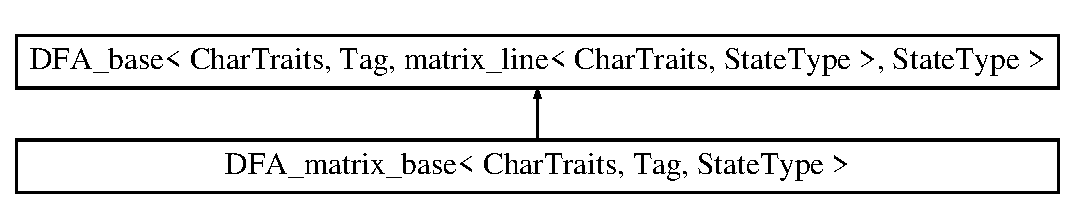
\includegraphics[height=2.000000cm]{classastl_1_1DFA__matrix__base}
\end{center}
\end{figure}
\subsection*{Public Member Functions}
\begin{DoxyCompactItemize}
\item 
const\+\_\+iterator {\bf begin} () const
\item 
void {\bf copy\+\_\+state} (state\+\_\+type from, state\+\_\+type to)
\begin{DoxyCompactList}\small\item\em Makes the state {\ttfamily to} an exact copy of the state {\ttfamily from}. \end{DoxyCompactList}\item 
void {\bf del\+\_\+state} (state\+\_\+type s)
\begin{DoxyCompactList}\small\item\em Destroyes the state {\ttfamily s}. \end{DoxyCompactList}\item 
state\+\_\+type {\bf duplicate\+\_\+state} (state\+\_\+type q)
\begin{DoxyCompactList}\small\item\em Allocates an exact copy of the state {\ttfamily q}. \end{DoxyCompactList}\item 
const\+\_\+iterator {\bf end} () const
\item 
bool {\bf final} (state\+\_\+type s) const
\item 
char \& {\bf final} (state\+\_\+type s)
\item 
void {\bf initial} (state\+\_\+type s)
\begin{DoxyCompactList}\small\item\em Sets the initial state of the automaton to {\ttfamily s}. \end{DoxyCompactList}\item 
state\+\_\+type {\bf initial} () const
\item 
state\+\_\+type {\bf new\+\_\+state} ()
\begin{DoxyCompactList}\small\item\em Allocates a new state structure. \end{DoxyCompactList}\item 
unsigned long {\bf state\+\_\+count} () const
\item 
tag\+\_\+type \& {\bf tag} (state\+\_\+type s)
\item 
const tag\+\_\+type \& {\bf tag} (state\+\_\+type s) const
\item 
unsigned long {\bf trans\+\_\+count} () const
\end{DoxyCompactItemize}


\subsection{Detailed Description}
\subsubsection*{template$<$class Char\+Traits = plain, class Tag = empty\+\_\+tag, class State\+Type = unsigned int$>$class astl\+::\+D\+F\+A\+\_\+matrix\+\_\+base$<$ Char\+Traits, Tag, State\+Type $>$}

A deterministic automaton container class that stores transitions targets in a matrix state x letter\+: each state has a line the size of the alphabet. 

It has a fast constant-\/time access to transitions but tends to consume too much memory space when the matrix is sparse. It is also not recommended for depth-\/ or breadth-\/first traversals.

This container is advisable for efficient pattern matching and for almost nothing else.

The constant-\/time access to transitions is provided by the character traits through the mapping between the alphabet and the integers implemented by {\ttfamily Char\+Traits\+::to\+\_\+char\+\_\+type()} and {\ttfamily Char\+Traits\+::to\+\_\+int\+\_\+type()}.

\begin{DoxyParagraph}{Template parameters}
\begin{TabularC}{4}
\hline
\rowcolor{lightgray}{\bf Parameter}&{\bf Description}&{\bf Default}&{\bf Requirements }\\\cline{1-4}
{\ttfamily Char\+Traits} &Character traits describing the letters that the transitions bear.&{\ttfamily plain} &{\ttfamily Char\+Traits} is a model of \#\+Enumerable\+Alphabet \\\cline{1-4}
{\ttfamily Tag} &The type of the data attached to states.&{\ttfamily empty\+\_\+tag} &\\\cline{1-4}
\end{TabularC}

\end{DoxyParagraph}


\subsection{Member Function Documentation}
\index{astl\+::\+D\+F\+A\+\_\+matrix\+\_\+base@{astl\+::\+D\+F\+A\+\_\+matrix\+\_\+base}!begin@{begin}}
\index{begin@{begin}!astl\+::\+D\+F\+A\+\_\+matrix\+\_\+base@{astl\+::\+D\+F\+A\+\_\+matrix\+\_\+base}}
\subsubsection[{begin}]{\setlength{\rightskip}{0pt plus 5cm}const\+\_\+iterator begin (
\begin{DoxyParamCaption}
{}
\end{DoxyParamCaption}
) const\hspace{0.3cm}{\ttfamily [inherited]}}\label{classastl_1_1DFA__base_aa4b02d4f1a8500fb07a551069060709f}
\begin{DoxyReturn}{Returns}
a forward iterator on the beginning of the sequence of the automaton states of type {\ttfamily state\+\_\+type} arranged in an undefined order (probably in allocation order but that is not a requirement). 
\end{DoxyReturn}
\index{astl\+::\+D\+F\+A\+\_\+matrix\+\_\+base@{astl\+::\+D\+F\+A\+\_\+matrix\+\_\+base}!copy\+\_\+state@{copy\+\_\+state}}
\index{copy\+\_\+state@{copy\+\_\+state}!astl\+::\+D\+F\+A\+\_\+matrix\+\_\+base@{astl\+::\+D\+F\+A\+\_\+matrix\+\_\+base}}
\subsubsection[{copy\+\_\+state}]{\setlength{\rightskip}{0pt plus 5cm}void copy\+\_\+state (
\begin{DoxyParamCaption}
\item[{{\bf state\+\_\+type}}]{from, }
\item[{{\bf state\+\_\+type}}]{to}
\end{DoxyParamCaption}
)\hspace{0.3cm}{\ttfamily [inherited]}}\label{classastl_1_1DFA__base_a4e3e0654b66dfe88b0a093de04437bec}


Makes the state {\ttfamily to} an exact copy of the state {\ttfamily from}. 

The tag and the transitions of {\ttfamily to} are destroyed and the new ones are copy-\/constructed from those of {\ttfamily from}. \begin{DoxyPrecond}{Precondition}
{\ttfamily from} has been returned by a previous call to {\ttfamily \doxyref{new\+\_\+state()}{p.}{classastl_1_1DFA__base_a252db8b50da681bd88660c6f1166f6c7}} 

{\ttfamily to} has been returned by a previous call to {\ttfamily \doxyref{new\+\_\+state()}{p.}{classastl_1_1DFA__base_a252db8b50da681bd88660c6f1166f6c7}} 
\end{DoxyPrecond}
\index{astl\+::\+D\+F\+A\+\_\+matrix\+\_\+base@{astl\+::\+D\+F\+A\+\_\+matrix\+\_\+base}!del\+\_\+state@{del\+\_\+state}}
\index{del\+\_\+state@{del\+\_\+state}!astl\+::\+D\+F\+A\+\_\+matrix\+\_\+base@{astl\+::\+D\+F\+A\+\_\+matrix\+\_\+base}}
\subsubsection[{del\+\_\+state}]{\setlength{\rightskip}{0pt plus 5cm}void del\+\_\+state (
\begin{DoxyParamCaption}
\item[{{\bf state\+\_\+type}}]{s}
\end{DoxyParamCaption}
)\hspace{0.3cm}{\ttfamily [inherited]}}\label{classastl_1_1DFA__base_a8bf68bf8c77e67ebfca27a8472e4c913}


Destroyes the state {\ttfamily s}. 

The tag and the transitions are destroyed. \begin{DoxyPrecond}{Precondition}
{\ttfamily s} has been returned by a previous call to {\ttfamily \doxyref{new\+\_\+state()}{p.}{classastl_1_1DFA__base_a252db8b50da681bd88660c6f1166f6c7}} 
\end{DoxyPrecond}
\index{astl\+::\+D\+F\+A\+\_\+matrix\+\_\+base@{astl\+::\+D\+F\+A\+\_\+matrix\+\_\+base}!duplicate\+\_\+state@{duplicate\+\_\+state}}
\index{duplicate\+\_\+state@{duplicate\+\_\+state}!astl\+::\+D\+F\+A\+\_\+matrix\+\_\+base@{astl\+::\+D\+F\+A\+\_\+matrix\+\_\+base}}
\subsubsection[{duplicate\+\_\+state}]{\setlength{\rightskip}{0pt plus 5cm}state\+\_\+type duplicate\+\_\+state (
\begin{DoxyParamCaption}
\item[{{\bf state\+\_\+type}}]{q}
\end{DoxyParamCaption}
)\hspace{0.3cm}{\ttfamily [inherited]}}\label{classastl_1_1DFA__base_a4788aa4f6e09d5b70bc2f3defabb1ea7}


Allocates an exact copy of the state {\ttfamily q}. 

\begin{DoxyReturn}{Returns}
the id of the freshly allocated state 
\end{DoxyReturn}
\begin{DoxyPrecond}{Precondition}
{\ttfamily q} has been returned by a previous call to {\ttfamily \doxyref{new\+\_\+state()}{p.}{classastl_1_1DFA__base_a252db8b50da681bd88660c6f1166f6c7}} 
\end{DoxyPrecond}
\index{astl\+::\+D\+F\+A\+\_\+matrix\+\_\+base@{astl\+::\+D\+F\+A\+\_\+matrix\+\_\+base}!end@{end}}
\index{end@{end}!astl\+::\+D\+F\+A\+\_\+matrix\+\_\+base@{astl\+::\+D\+F\+A\+\_\+matrix\+\_\+base}}
\subsubsection[{end}]{\setlength{\rightskip}{0pt plus 5cm}const\+\_\+iterator end (
\begin{DoxyParamCaption}
{}
\end{DoxyParamCaption}
) const\hspace{0.3cm}{\ttfamily [inherited]}}\label{classastl_1_1DFA__base_a350132543d80a1c1e5be844e6d2878ea}
\begin{DoxyReturn}{Returns}
a past-\/the-\/end forward iterator on the sequence of the automaton states. 
\end{DoxyReturn}
\index{astl\+::\+D\+F\+A\+\_\+matrix\+\_\+base@{astl\+::\+D\+F\+A\+\_\+matrix\+\_\+base}!final@{final}}
\index{final@{final}!astl\+::\+D\+F\+A\+\_\+matrix\+\_\+base@{astl\+::\+D\+F\+A\+\_\+matrix\+\_\+base}}
\subsubsection[{final}]{\setlength{\rightskip}{0pt plus 5cm}bool final (
\begin{DoxyParamCaption}
\item[{{\bf state\+\_\+type}}]{s}
\end{DoxyParamCaption}
) const\hspace{0.3cm}{\ttfamily [inherited]}}\label{classastl_1_1DFA__base_ad1882121c53bdedd74df649d71b70a4c}
\begin{DoxyReturn}{Returns}
{\ttfamily true} if {\ttfamily s} is a final state. 
\end{DoxyReturn}
\begin{DoxyPrecond}{Precondition}
{\ttfamily s} has been returned by a previous call to {\ttfamily \doxyref{new\+\_\+state()}{p.}{classastl_1_1DFA__base_a252db8b50da681bd88660c6f1166f6c7}} 
\end{DoxyPrecond}
\index{astl\+::\+D\+F\+A\+\_\+matrix\+\_\+base@{astl\+::\+D\+F\+A\+\_\+matrix\+\_\+base}!final@{final}}
\index{final@{final}!astl\+::\+D\+F\+A\+\_\+matrix\+\_\+base@{astl\+::\+D\+F\+A\+\_\+matrix\+\_\+base}}
\subsubsection[{final}]{\setlength{\rightskip}{0pt plus 5cm}char\& final (
\begin{DoxyParamCaption}
\item[{{\bf state\+\_\+type}}]{s}
\end{DoxyParamCaption}
)\hspace{0.3cm}{\ttfamily [inherited]}}\label{classastl_1_1DFA__base_a8011bf53b33ceac2c71ca364bbb1fbc3}
\begin{DoxyReturn}{Returns}
a reference to a boolean that, if assigned {\ttfamily true} sets the state {\ttfamily s} to be a final state and if assigned {\ttfamily false} sets {\ttfamily s} to be a non-\/final state. 
\end{DoxyReturn}
\begin{DoxyPrecond}{Precondition}
{\ttfamily s} has been returned by a previous call to {\ttfamily \doxyref{new\+\_\+state()}{p.}{classastl_1_1DFA__base_a252db8b50da681bd88660c6f1166f6c7}} 
\end{DoxyPrecond}
\index{astl\+::\+D\+F\+A\+\_\+matrix\+\_\+base@{astl\+::\+D\+F\+A\+\_\+matrix\+\_\+base}!initial@{initial}}
\index{initial@{initial}!astl\+::\+D\+F\+A\+\_\+matrix\+\_\+base@{astl\+::\+D\+F\+A\+\_\+matrix\+\_\+base}}
\subsubsection[{initial}]{\setlength{\rightskip}{0pt plus 5cm}void initial (
\begin{DoxyParamCaption}
\item[{{\bf state\+\_\+type}}]{s}
\end{DoxyParamCaption}
)\hspace{0.3cm}{\ttfamily [inherited]}}\label{classastl_1_1DFA__base_a0512d51289bf8ed1a0d42df6272c0d70}


Sets the initial state of the automaton to {\ttfamily s}. 

\begin{DoxyPrecond}{Precondition}
{\ttfamily s} has been returned by a previous call to {\ttfamily \doxyref{new\+\_\+state()}{p.}{classastl_1_1DFA__base_a252db8b50da681bd88660c6f1166f6c7}} 
\end{DoxyPrecond}
\begin{DoxyPostcond}{Postcondition}

\begin{DoxyCode}
initial() == s 
\end{DoxyCode}
 
\end{DoxyPostcond}
\index{astl\+::\+D\+F\+A\+\_\+matrix\+\_\+base@{astl\+::\+D\+F\+A\+\_\+matrix\+\_\+base}!initial@{initial}}
\index{initial@{initial}!astl\+::\+D\+F\+A\+\_\+matrix\+\_\+base@{astl\+::\+D\+F\+A\+\_\+matrix\+\_\+base}}
\subsubsection[{initial}]{\setlength{\rightskip}{0pt plus 5cm}state\+\_\+type initial (
\begin{DoxyParamCaption}
{}
\end{DoxyParamCaption}
) const\hspace{0.3cm}{\ttfamily [inherited]}}\label{classastl_1_1DFA__base_a4edaf60fafcacf017837f0a5eb5bc39b}
\begin{DoxyReturn}{Returns}
the initial state of the automaton. 
\end{DoxyReturn}
\index{astl\+::\+D\+F\+A\+\_\+matrix\+\_\+base@{astl\+::\+D\+F\+A\+\_\+matrix\+\_\+base}!new\+\_\+state@{new\+\_\+state}}
\index{new\+\_\+state@{new\+\_\+state}!astl\+::\+D\+F\+A\+\_\+matrix\+\_\+base@{astl\+::\+D\+F\+A\+\_\+matrix\+\_\+base}}
\subsubsection[{new\+\_\+state}]{\setlength{\rightskip}{0pt plus 5cm}state\+\_\+type new\+\_\+state (
\begin{DoxyParamCaption}
{}
\end{DoxyParamCaption}
)\hspace{0.3cm}{\ttfamily [inherited]}}\label{classastl_1_1DFA__base_a252db8b50da681bd88660c6f1166f6c7}


Allocates a new state structure. 

The newly created state is non-\/final and has no transitions. The tag is default-\/constructed. \begin{DoxyReturn}{Returns}
the id of the freshly allocated state 
\end{DoxyReturn}
\index{astl\+::\+D\+F\+A\+\_\+matrix\+\_\+base@{astl\+::\+D\+F\+A\+\_\+matrix\+\_\+base}!state\+\_\+count@{state\+\_\+count}}
\index{state\+\_\+count@{state\+\_\+count}!astl\+::\+D\+F\+A\+\_\+matrix\+\_\+base@{astl\+::\+D\+F\+A\+\_\+matrix\+\_\+base}}
\subsubsection[{state\+\_\+count}]{\setlength{\rightskip}{0pt plus 5cm}unsigned long state\+\_\+count (
\begin{DoxyParamCaption}
{}
\end{DoxyParamCaption}
) const\hspace{0.3cm}{\ttfamily [inherited]}}\label{classastl_1_1DFA__base_abbd3928d673458d0fa63e568a950a83d}
\begin{DoxyReturn}{Returns}
the number of states in the automaton 
\end{DoxyReturn}
\index{astl\+::\+D\+F\+A\+\_\+matrix\+\_\+base@{astl\+::\+D\+F\+A\+\_\+matrix\+\_\+base}!tag@{tag}}
\index{tag@{tag}!astl\+::\+D\+F\+A\+\_\+matrix\+\_\+base@{astl\+::\+D\+F\+A\+\_\+matrix\+\_\+base}}
\subsubsection[{tag}]{\setlength{\rightskip}{0pt plus 5cm}tag\+\_\+type\& tag (
\begin{DoxyParamCaption}
\item[{{\bf state\+\_\+type}}]{s}
\end{DoxyParamCaption}
)\hspace{0.3cm}{\ttfamily [inherited]}}\label{classastl_1_1DFA__base_a3dd4257038bc77fa1cc7d9bf0afc29d5}
\begin{DoxyReturn}{Returns}
the data attached to the state {\ttfamily s} 
\end{DoxyReturn}
\begin{DoxyPrecond}{Precondition}
{\ttfamily s} has been returned by a previous call to {\ttfamily \doxyref{new\+\_\+state()}{p.}{classastl_1_1DFA__base_a252db8b50da681bd88660c6f1166f6c7}} 
\end{DoxyPrecond}
\index{astl\+::\+D\+F\+A\+\_\+matrix\+\_\+base@{astl\+::\+D\+F\+A\+\_\+matrix\+\_\+base}!tag@{tag}}
\index{tag@{tag}!astl\+::\+D\+F\+A\+\_\+matrix\+\_\+base@{astl\+::\+D\+F\+A\+\_\+matrix\+\_\+base}}
\subsubsection[{tag}]{\setlength{\rightskip}{0pt plus 5cm}const tag\+\_\+type\& tag (
\begin{DoxyParamCaption}
\item[{{\bf state\+\_\+type}}]{s}
\end{DoxyParamCaption}
) const\hspace{0.3cm}{\ttfamily [inherited]}}\label{classastl_1_1DFA__base_aae6988f0a4fda8a527b52781ab9f0d59}
\begin{DoxyReturn}{Returns}
the data attached to the state {\ttfamily s} 
\end{DoxyReturn}
\begin{DoxyPrecond}{Precondition}
{\ttfamily s} has been returned by a previous call to {\ttfamily \doxyref{new\+\_\+state()}{p.}{classastl_1_1DFA__base_a252db8b50da681bd88660c6f1166f6c7}} 
\end{DoxyPrecond}
\index{astl\+::\+D\+F\+A\+\_\+matrix\+\_\+base@{astl\+::\+D\+F\+A\+\_\+matrix\+\_\+base}!trans\+\_\+count@{trans\+\_\+count}}
\index{trans\+\_\+count@{trans\+\_\+count}!astl\+::\+D\+F\+A\+\_\+matrix\+\_\+base@{astl\+::\+D\+F\+A\+\_\+matrix\+\_\+base}}
\subsubsection[{trans\+\_\+count}]{\setlength{\rightskip}{0pt plus 5cm}unsigned long trans\+\_\+count (
\begin{DoxyParamCaption}
{}
\end{DoxyParamCaption}
) const\hspace{0.3cm}{\ttfamily [inherited]}}\label{classastl_1_1DFA__base_a3f2590089bd23eb738c72bf9acfb9c44}
\begin{DoxyReturn}{Returns}
the number of transitions in the automaton 
\end{DoxyReturn}

\section{D\+F\+A\+\_\+min$<$ Char\+Traits, Tag $>$ Class Template Reference}
\label{classastl_1_1DFA__min}\index{D\+F\+A\+\_\+min$<$ Char\+Traits, Tag $>$@{D\+F\+A\+\_\+min$<$ Char\+Traits, Tag $>$}}


A dynamic minimal acyclic D\+F\+A container class.  




{\ttfamily \#include $<$dfa\+\_\+min.\+h$>$}



Inherits D\+F\+A\+\_\+concept.

\subsection*{Public Member Functions}
\begin{DoxyCompactItemize}
\item 
void {\bf clear} ()
\item 
void {\bf freeze} ()
\begin{DoxyCompactList}\small\item\em Get rid of the extra data used for maintaining the automaton minimality. \end{DoxyCompactList}\item 
{\footnotesize template$<$class Forward\+I $>$ }\\bool {\bf insert} (Forward\+I, Forward\+I)
\begin{DoxyCompactList}\small\item\em Add a word defined by a range on a sequence of characters of type {\ttfamily char\+\_\+type}. \end{DoxyCompactList}\item 
bool {\bf insert} (const basic\+\_\+string$<$ char\+\_\+type $>$ \&s)
\begin{DoxyCompactList}\small\item\em Add a word defined by a character string. \end{DoxyCompactList}\item 
unsigned int {\bf size} () const 
\item 
unsigned int {\bf wc} () const 
\begin{DoxyCompactList}\small\item\em word count. \end{DoxyCompactList}\end{DoxyCompactItemize}


\subsection{Detailed Description}
\subsubsection*{template$<$typename Char\+Traits = plain, typename Tag = empty\+\_\+tag$>$class astl\+::\+D\+F\+A\+\_\+min$<$ Char\+Traits, Tag $>$}

A dynamic minimal acyclic D\+F\+A container class. 

Words can be added keeping the automaton minimal. It does not define the standard D\+F\+A interface but a restricted one that allows only word insertions and read-\/only operations thus enforcing the invariants for the structure integrity to be guaranteed.

\begin{DoxyParagraph}{Template parameters}
\begin{TabularC}{4}
\hline
\rowcolor{lightgray}{\bf Parameter}&{\bf Description}&{\bf Default}&{\bf Requirements }\\\cline{1-4}
{\ttfamily Char\+Traits} &Character traits describing the alphabet that the words are built with.&{\ttfamily plain} &{\ttfamily Char\+Traits} is a model of \#\+Alphabet and {\ttfamily Char\+Traits\+::char\+\_\+type} is a P\+O\+D type \\\cline{1-4}
{\ttfamily Tag} &The type of the data attached to states.&{\ttfamily empty\+\_\+tag}  &\\\cline{1-4}
\end{TabularC}

\end{DoxyParagraph}


\subsection{Member Function Documentation}
\index{astl\+::\+D\+F\+A\+\_\+min@{astl\+::\+D\+F\+A\+\_\+min}!clear@{clear}}
\index{clear@{clear}!astl\+::\+D\+F\+A\+\_\+min@{astl\+::\+D\+F\+A\+\_\+min}}
\subsubsection[{clear}]{\setlength{\rightskip}{0pt plus 5cm}void clear (
\begin{DoxyParamCaption}
{}
\end{DoxyParamCaption}
)}\label{classastl_1_1DFA__min_ac8bb3912a3ce86b15842e79d0b421204}
\begin{DoxyPostcond}{Postcondition}

\begin{DoxyCode}
wc() == 0 
\end{DoxyCode}
 
\end{DoxyPostcond}
\index{astl\+::\+D\+F\+A\+\_\+min@{astl\+::\+D\+F\+A\+\_\+min}!freeze@{freeze}}
\index{freeze@{freeze}!astl\+::\+D\+F\+A\+\_\+min@{astl\+::\+D\+F\+A\+\_\+min}}
\subsubsection[{freeze}]{\setlength{\rightskip}{0pt plus 5cm}void freeze (
\begin{DoxyParamCaption}
{}
\end{DoxyParamCaption}
)}\label{classastl_1_1DFA__min_abd8698b462ce90fe56b15ce7a0192d3e}


Get rid of the extra data used for maintaining the automaton minimality. 

Once frozen, words can still be added but the next insertion will take more time to rebuild the necessary data structure that had been disposed of. \index{astl\+::\+D\+F\+A\+\_\+min@{astl\+::\+D\+F\+A\+\_\+min}!insert@{insert}}
\index{insert@{insert}!astl\+::\+D\+F\+A\+\_\+min@{astl\+::\+D\+F\+A\+\_\+min}}
\subsubsection[{insert}]{\setlength{\rightskip}{0pt plus 5cm}bool insert (
\begin{DoxyParamCaption}
\item[{Forward\+I}]{, }
\item[{Forward\+I}]{}
\end{DoxyParamCaption}
)}\label{classastl_1_1DFA__min_a3a43f9279038d8072b59af3c45b9b9fb}


Add a word defined by a range on a sequence of characters of type {\ttfamily char\+\_\+type}. 

\begin{DoxyReturn}{Returns}
{\ttfamily true} if the word has been actually added, {\ttfamily false} if the word already exists and that the operation left the automaton unchanged. 
\end{DoxyReturn}
\begin{DoxyPostcond}{Postcondition}
the automaton is minimal. 
\end{DoxyPostcond}
\index{astl\+::\+D\+F\+A\+\_\+min@{astl\+::\+D\+F\+A\+\_\+min}!insert@{insert}}
\index{insert@{insert}!astl\+::\+D\+F\+A\+\_\+min@{astl\+::\+D\+F\+A\+\_\+min}}
\subsubsection[{insert}]{\setlength{\rightskip}{0pt plus 5cm}bool insert (
\begin{DoxyParamCaption}
\item[{const basic\+\_\+string$<$ char\+\_\+type $>$ \&}]{s}
\end{DoxyParamCaption}
)}\label{classastl_1_1DFA__min_a2c5644df13a4cb77ac2120138ca5df54}


Add a word defined by a character string. 

\begin{DoxyReturn}{Returns}
{\ttfamily true} if the word has been actually added, {\ttfamily false} if the word already exists and that the operation left the automaton unchanged. 
\end{DoxyReturn}
\begin{DoxyPostcond}{Postcondition}
the automaton is minimal. 
\end{DoxyPostcond}
\index{astl\+::\+D\+F\+A\+\_\+min@{astl\+::\+D\+F\+A\+\_\+min}!size@{size}}
\index{size@{size}!astl\+::\+D\+F\+A\+\_\+min@{astl\+::\+D\+F\+A\+\_\+min}}
\subsubsection[{size}]{\setlength{\rightskip}{0pt plus 5cm}unsigned int size (
\begin{DoxyParamCaption}
{}
\end{DoxyParamCaption}
) const}\label{classastl_1_1DFA__min_a90ca964ebcc1b02bbcde225edd49e812}
\begin{DoxyReturn}{Returns}
{\ttfamily \doxyref{wc()}{p.}{classastl_1_1DFA__min_a5bc74fdaa5f23bc3e8e6479f9cac6203}} 
\end{DoxyReturn}
\index{astl\+::\+D\+F\+A\+\_\+min@{astl\+::\+D\+F\+A\+\_\+min}!wc@{wc}}
\index{wc@{wc}!astl\+::\+D\+F\+A\+\_\+min@{astl\+::\+D\+F\+A\+\_\+min}}
\subsubsection[{wc}]{\setlength{\rightskip}{0pt plus 5cm}unsigned int wc (
\begin{DoxyParamCaption}
{}
\end{DoxyParamCaption}
) const}\label{classastl_1_1DFA__min_a5bc74fdaa5f23bc3e8e6479f9cac6203}


word count. 

\begin{DoxyReturn}{Returns}
a count of the words in the automaton language 
\end{DoxyReturn}

\section{D\+F\+A\+\_\+min\+\_\+hash$<$ Char\+Traits $>$ Class Template Reference}
\label{classastl_1_1DFA__min__hash}\index{D\+F\+A\+\_\+min\+\_\+hash$<$ Char\+Traits $>$@{D\+F\+A\+\_\+min\+\_\+hash$<$ Char\+Traits $>$}}


A perfect hashing function from words (sequences of characters) to integers and from integers to words.  




{\ttfamily \#include $<$dfa\+\_\+min\+\_\+hash.\+h$>$}

Inheritance diagram for D\+F\+A\+\_\+min\+\_\+hash$<$ Char\+Traits $>$\+:\begin{figure}[H]
\begin{center}
\leavevmode
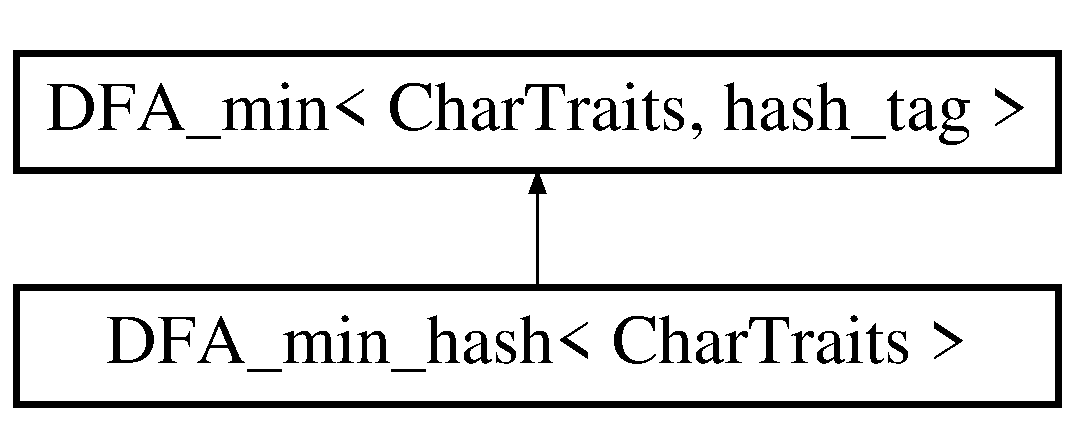
\includegraphics[height=2.000000cm]{classastl_1_1DFA__min__hash}
\end{center}
\end{figure}
\subsection*{Public Member Functions}
\begin{DoxyCompactItemize}
\item 
void {\bf clear} ()
\item 
void {\bf freeze} ()
\begin{DoxyCompactList}\small\item\em Get rid of the extra data used for maintaining the automaton minimality. \end{DoxyCompactList}\item 
{\footnotesize template$<$typename Input\+I $>$ }\\int {\bf hash\+\_\+value} (Input\+I first, Input\+I last) const 
\begin{DoxyCompactList}\small\item\em Get the hash value for the word passed as a range of characters of type {\ttfamily char\+\_\+type}. \end{DoxyCompactList}\item 
int {\bf hash\+\_\+value} (const basic\+\_\+string$<$ char\+\_\+type $>$ \&s) const 
\begin{DoxyCompactList}\small\item\em Get the hash value for the word passed as a character string. \end{DoxyCompactList}\item 
{\footnotesize template$<$class Forward\+I $>$ }\\bool {\bf insert} (Forward\+I, Forward\+I)
\begin{DoxyCompactList}\small\item\em Add a word defined by a range on a sequence of characters of type {\ttfamily char\+\_\+type}. \end{DoxyCompactList}\item 
bool {\bf insert} (const basic\+\_\+string$<$ char\+\_\+type $>$ \&s)
\begin{DoxyCompactList}\small\item\em Add a word defined by a character string. \end{DoxyCompactList}\item 
unsigned int {\bf size} () const
\item 
{\footnotesize template$<$typename Output\+I $>$ }\\int {\bf value\+\_\+hash} (int w, Output\+I out) const 
\begin{DoxyCompactList}\small\item\em Get the word for the hash value {\ttfamily w} as a sequence of characters of type {\ttfamily char\+\_\+type} written out through the output iterator {\ttfamily out}. \end{DoxyCompactList}\item 
basic\+\_\+string$<$ char\+\_\+type $>$ {\bf value\+\_\+hash} (int w) const 
\begin{DoxyCompactList}\small\item\em Get the word for the hash value {\ttfamily w} as a character string. \end{DoxyCompactList}\item 
unsigned int {\bf wc} () const
\begin{DoxyCompactList}\small\item\em word count. \end{DoxyCompactList}\end{DoxyCompactItemize}


\subsection{Detailed Description}
\subsubsection*{template$<$typename Char\+Traits = plain$>$class astl\+::\+D\+F\+A\+\_\+min\+\_\+hash$<$ Char\+Traits $>$}

A perfect hashing function from words (sequences of characters) to integers and from integers to words. 

The hashing is implemented with a dynamic minimal acyclic D\+F\+A and maps words to strictly positive integers in lexicographical order. This order is determined by the ordering defined on characters in the static method {\ttfamily Char\+Traits\+::lt}. Therefore, the mapping is not stable with respect to the insertion\+: a new word will be associated to its position in the lexicographically-\/sorted word list, thus shifting by an offset of 1 all mappings beyond the insertion position. The set of words must then be fixed for this hashing function to be usable.

This class does not define the standard D\+F\+A interface but a restricted one that allows only word insertions and read-\/only operations thus enforcing the invariants for the structure integrity to be guaranteed.

\begin{DoxyParagraph}{Template parameters}
\begin{TabularC}{4}
\hline
\rowcolor{lightgray}{\bf Parameter}&{\bf Description}&{\bf Default}&{\bf Requirements }\\\cline{1-4}
{\ttfamily Char\+Traits} &Character traits describing the alphabet that the words are built with.&{\ttfamily plain} &{\ttfamily Char\+Traits} is a model of \#\+Alphabet\\\cline{1-4}
\end{TabularC}

\end{DoxyParagraph}


\subsection{Member Function Documentation}
\index{astl\+::\+D\+F\+A\+\_\+min\+\_\+hash@{astl\+::\+D\+F\+A\+\_\+min\+\_\+hash}!clear@{clear}}
\index{clear@{clear}!astl\+::\+D\+F\+A\+\_\+min\+\_\+hash@{astl\+::\+D\+F\+A\+\_\+min\+\_\+hash}}
\subsubsection[{clear}]{\setlength{\rightskip}{0pt plus 5cm}void clear (
\begin{DoxyParamCaption}
{}
\end{DoxyParamCaption}
)\hspace{0.3cm}{\ttfamily [inherited]}}\label{classastl_1_1DFA__min_ac8bb3912a3ce86b15842e79d0b421204}
\begin{DoxyPostcond}{Postcondition}

\begin{DoxyCode}
wc() == 0 
\end{DoxyCode}
 
\end{DoxyPostcond}
\index{astl\+::\+D\+F\+A\+\_\+min\+\_\+hash@{astl\+::\+D\+F\+A\+\_\+min\+\_\+hash}!freeze@{freeze}}
\index{freeze@{freeze}!astl\+::\+D\+F\+A\+\_\+min\+\_\+hash@{astl\+::\+D\+F\+A\+\_\+min\+\_\+hash}}
\subsubsection[{freeze}]{\setlength{\rightskip}{0pt plus 5cm}void freeze (
\begin{DoxyParamCaption}
{}
\end{DoxyParamCaption}
)\hspace{0.3cm}{\ttfamily [inherited]}}\label{classastl_1_1DFA__min_abd8698b462ce90fe56b15ce7a0192d3e}


Get rid of the extra data used for maintaining the automaton minimality. 

Once frozen, words can still be added but the next insertion will take more time to rebuild the necessary data structure that had been disposed of. \index{astl\+::\+D\+F\+A\+\_\+min\+\_\+hash@{astl\+::\+D\+F\+A\+\_\+min\+\_\+hash}!hash\+\_\+value@{hash\+\_\+value}}
\index{hash\+\_\+value@{hash\+\_\+value}!astl\+::\+D\+F\+A\+\_\+min\+\_\+hash@{astl\+::\+D\+F\+A\+\_\+min\+\_\+hash}}
\subsubsection[{hash\+\_\+value}]{\setlength{\rightskip}{0pt plus 5cm}int hash\+\_\+value (
\begin{DoxyParamCaption}
\item[{Input\+I}]{first, }
\item[{Input\+I}]{last}
\end{DoxyParamCaption}
) const}\label{classastl_1_1DFA__min__hash_a769253952109eb60c035684032bd36fb}


Get the hash value for the word passed as a range of characters of type {\ttfamily char\+\_\+type}. 

\begin{DoxyReturn}{Returns}
the integer associated with the word if found, 0 otherwise. 
\end{DoxyReturn}
\index{astl\+::\+D\+F\+A\+\_\+min\+\_\+hash@{astl\+::\+D\+F\+A\+\_\+min\+\_\+hash}!hash\+\_\+value@{hash\+\_\+value}}
\index{hash\+\_\+value@{hash\+\_\+value}!astl\+::\+D\+F\+A\+\_\+min\+\_\+hash@{astl\+::\+D\+F\+A\+\_\+min\+\_\+hash}}
\subsubsection[{hash\+\_\+value}]{\setlength{\rightskip}{0pt plus 5cm}int hash\+\_\+value (
\begin{DoxyParamCaption}
\item[{const basic\+\_\+string$<$ char\+\_\+type $>$ \&}]{s}
\end{DoxyParamCaption}
) const}\label{classastl_1_1DFA__min__hash_ad9a99dc33cd0843108d8acbf64c1d5b4}


Get the hash value for the word passed as a character string. 

\begin{DoxyReturn}{Returns}
the integer associated with the word if found, 0 otherwise. 
\end{DoxyReturn}
\index{astl\+::\+D\+F\+A\+\_\+min\+\_\+hash@{astl\+::\+D\+F\+A\+\_\+min\+\_\+hash}!insert@{insert}}
\index{insert@{insert}!astl\+::\+D\+F\+A\+\_\+min\+\_\+hash@{astl\+::\+D\+F\+A\+\_\+min\+\_\+hash}}
\subsubsection[{insert}]{\setlength{\rightskip}{0pt plus 5cm}bool insert (
\begin{DoxyParamCaption}
\item[{Forward\+I}]{first, }
\item[{Forward\+I}]{last}
\end{DoxyParamCaption}
)}\label{classastl_1_1DFA__min__hash_a3a43f9279038d8072b59af3c45b9b9fb}


Add a word defined by a range on a sequence of characters of type {\ttfamily char\+\_\+type}. 

\begin{DoxyReturn}{Returns}
{\ttfamily true} if the word has been actually added, {\ttfamily false} if the word already exists and that the operation left the automaton unchanged. 
\end{DoxyReturn}


References stack\+\_\+cursor$<$ Forward\+Cursor, Stack\+Container $>$\+::aim(), stack\+\_\+cursor$<$ Forward\+Cursor, Stack\+Container $>$\+::backward(), stack\+\_\+cursor$<$ Forward\+Cursor, Stack\+Container $>$\+::find(), stack\+\_\+cursor$<$ Forward\+Cursor, Stack\+Container $>$\+::forward(), stack\+\_\+cursor$<$ Forward\+Cursor, Stack\+Container $>$\+::letter(), and stack\+\_\+cursor$<$ Forward\+Cursor, Stack\+Container $>$\+::src().

\index{astl\+::\+D\+F\+A\+\_\+min\+\_\+hash@{astl\+::\+D\+F\+A\+\_\+min\+\_\+hash}!insert@{insert}}
\index{insert@{insert}!astl\+::\+D\+F\+A\+\_\+min\+\_\+hash@{astl\+::\+D\+F\+A\+\_\+min\+\_\+hash}}
\subsubsection[{insert}]{\setlength{\rightskip}{0pt plus 5cm}bool insert (
\begin{DoxyParamCaption}
\item[{const basic\+\_\+string$<$ char\+\_\+type $>$ \&}]{s}
\end{DoxyParamCaption}
)}\label{classastl_1_1DFA__min__hash_a2c5644df13a4cb77ac2120138ca5df54}


Add a word defined by a character string. 

\begin{DoxyReturn}{Returns}
{\ttfamily true} if the word has been actually added, {\ttfamily false} if the word already exists and that the operation left the automaton unchanged. 
\end{DoxyReturn}
\index{astl\+::\+D\+F\+A\+\_\+min\+\_\+hash@{astl\+::\+D\+F\+A\+\_\+min\+\_\+hash}!size@{size}}
\index{size@{size}!astl\+::\+D\+F\+A\+\_\+min\+\_\+hash@{astl\+::\+D\+F\+A\+\_\+min\+\_\+hash}}
\subsubsection[{size}]{\setlength{\rightskip}{0pt plus 5cm}unsigned int size (
\begin{DoxyParamCaption}
{}
\end{DoxyParamCaption}
) const\hspace{0.3cm}{\ttfamily [inherited]}}\label{classastl_1_1DFA__min_a90ca964ebcc1b02bbcde225edd49e812}
\begin{DoxyReturn}{Returns}
{\ttfamily \doxyref{wc()}{p.}{classastl_1_1DFA__min_a5bc74fdaa5f23bc3e8e6479f9cac6203}} 
\end{DoxyReturn}
\index{astl\+::\+D\+F\+A\+\_\+min\+\_\+hash@{astl\+::\+D\+F\+A\+\_\+min\+\_\+hash}!value\+\_\+hash@{value\+\_\+hash}}
\index{value\+\_\+hash@{value\+\_\+hash}!astl\+::\+D\+F\+A\+\_\+min\+\_\+hash@{astl\+::\+D\+F\+A\+\_\+min\+\_\+hash}}
\subsubsection[{value\+\_\+hash}]{\setlength{\rightskip}{0pt plus 5cm}int value\+\_\+hash (
\begin{DoxyParamCaption}
\item[{int}]{w, }
\item[{Output\+I}]{out}
\end{DoxyParamCaption}
) const}\label{classastl_1_1DFA__min__hash_a8af10d0a82911469cc427e7d316a4883}


Get the word for the hash value {\ttfamily w} as a sequence of characters of type {\ttfamily char\+\_\+type} written out through the output iterator {\ttfamily out}. 

\begin{DoxyReturn}{Returns}
the length of the output sequence. 
\end{DoxyReturn}
\index{astl\+::\+D\+F\+A\+\_\+min\+\_\+hash@{astl\+::\+D\+F\+A\+\_\+min\+\_\+hash}!value\+\_\+hash@{value\+\_\+hash}}
\index{value\+\_\+hash@{value\+\_\+hash}!astl\+::\+D\+F\+A\+\_\+min\+\_\+hash@{astl\+::\+D\+F\+A\+\_\+min\+\_\+hash}}
\subsubsection[{value\+\_\+hash}]{\setlength{\rightskip}{0pt plus 5cm}basic\+\_\+string$<$char\+\_\+type$>$ value\+\_\+hash (
\begin{DoxyParamCaption}
\item[{int}]{w}
\end{DoxyParamCaption}
) const}\label{classastl_1_1DFA__min__hash_ad726952357dde6af24007542239012e6}


Get the word for the hash value {\ttfamily w} as a character string. 

\begin{DoxyReturn}{Returns}
the word that {\ttfamily w} is associated to. 
\end{DoxyReturn}
\index{astl\+::\+D\+F\+A\+\_\+min\+\_\+hash@{astl\+::\+D\+F\+A\+\_\+min\+\_\+hash}!wc@{wc}}
\index{wc@{wc}!astl\+::\+D\+F\+A\+\_\+min\+\_\+hash@{astl\+::\+D\+F\+A\+\_\+min\+\_\+hash}}
\subsubsection[{wc}]{\setlength{\rightskip}{0pt plus 5cm}unsigned int wc (
\begin{DoxyParamCaption}
{}
\end{DoxyParamCaption}
) const\hspace{0.3cm}{\ttfamily [inherited]}}\label{classastl_1_1DFA__min_a5bc74fdaa5f23bc3e8e6479f9cac6203}


word count. 

\begin{DoxyReturn}{Returns}
a count of the words in the automaton language 
\end{DoxyReturn}

\section{dfirst\+\_\+cursor$<$ Stack\+Cursor, Marker\+Function $>$ Class Template Reference}
\label{classastl_1_1dfirst__cursor}\index{dfirst\+\_\+cursor$<$ Stack\+Cursor, Marker\+Function $>$@{dfirst\+\_\+cursor$<$ Stack\+Cursor, Marker\+Function $>$}}


Implements the depth-\/first traversal on deterministic automata.  




{\ttfamily \#include $<$cursor.\+h$>$}



Inherits dfirst\+\_\+cursor\+\_\+concept.

\subsection*{Public Types}
\begin{DoxyCompactItemize}
\item 
typedef Stack\+Cursor\+::char\+\_\+traits {\bf char\+\_\+traits}\label{classastl_1_1dfirst__cursor_a78d7212db34e630f2fee7bcf834e80fa}

\begin{DoxyCompactList}\small\item\em Character traits describing \doxyref{char\+\_\+type}{p.}{classastl_1_1dfirst__cursor_ae3b8ebeb825ea3a141a33f2a4ae78dc2}. \end{DoxyCompactList}\item 
typedef Stack\+Cursor\+::char\+\_\+type {\bf char\+\_\+type}\label{classastl_1_1dfirst__cursor_ae3b8ebeb825ea3a141a33f2a4ae78dc2}

\begin{DoxyCompactList}\small\item\em The type of the transitions letters. \end{DoxyCompactList}\item 
typedef Stack\+Cursor\+::state\+\_\+type {\bf state\+\_\+type}\label{classastl_1_1dfirst__cursor_a10ee892449f2dbaaa1a4dc414fdb3a40}

\begin{DoxyCompactList}\small\item\em The type of the automaton-\/states identifiers. \end{DoxyCompactList}\item 
typedef Stack\+Cursor\+::tag\+\_\+type {\bf tag\+\_\+type}\label{classastl_1_1dfirst__cursor_a23fdec464051e2a276283141b68a151b}

\begin{DoxyCompactList}\small\item\em The type of the data attached to states. \end{DoxyCompactList}\end{DoxyCompactItemize}
\subsection*{Public Member Functions}
\begin{DoxyCompactItemize}
\item 
{\bf state\+\_\+type} {\bf aim} () const 
\begin{DoxyCompactList}\small\item\em Returns the aim state of the pointed transition. \end{DoxyCompactList}\item 
bool {\bf aim\+\_\+final} () const 
\begin{DoxyCompactList}\small\item\em Returns {\ttfamily true} if the aim state of the transition that this cursor points to is final. \end{DoxyCompactList}\item 
{\bf tag\+\_\+type} {\bf aim\+\_\+tag} () const 
\begin{DoxyCompactList}\small\item\em Returns the data attached to the aim state of the pointed transition. \end{DoxyCompactList}\item 
void {\bf backward} ()\label{classastl_1_1dfirst__cursor_a9b83f0fc7f06bee951213dd4b22e0e93}

\begin{DoxyCompactList}\small\item\em Forces the cursor to act as if there was no more transitions to push. \end{DoxyCompactList}\item 
{\bf dfirst\+\_\+cursor} (const Stack\+Cursor \&x, const Marker\+Function \&f=Marker\+Function())\label{classastl_1_1dfirst__cursor_ac22a17929dfd1bb0813a0de9ab06b063}

\begin{DoxyCompactList}\small\item\em Creates a cursor with {\ttfamily x} as stack. \end{DoxyCompactList}\item 
{\bf dfirst\+\_\+cursor} ()\label{classastl_1_1dfirst__cursor_a8c630c20d1fd900787926f900bc1ed18}

\begin{DoxyCompactList}\small\item\em Creates a cursor with an empty stack used as an end-\/of-\/range iterator. \end{DoxyCompactList}\item 
bool {\bf forward} ()
\begin{DoxyCompactList}\small\item\em Increments the cursor making it point to the next transition in the sequence. \end{DoxyCompactList}\item 
{\bf char\+\_\+type} {\bf letter} () const 
\begin{DoxyCompactList}\small\item\em Returns the letter on the pointed transition. \end{DoxyCompactList}\item 
bool {\bf operator!=} (const {\bf self} \&x) const \label{classastl_1_1dfirst__cursor_aef9934be5de2e5c7dd83e1a6a71fd607}

\begin{DoxyCompactList}\small\item\em Returns {\ttfamily true} if stacks are different. \end{DoxyCompactList}\item 
bool {\bf operator==} (const {\bf self} \&x) const \label{classastl_1_1dfirst__cursor_a8a0948685b8eb65ce6775c8f12547439}

\begin{DoxyCompactList}\small\item\em Returns {\ttfamily true} if both stacks are equal. \end{DoxyCompactList}\item 
{\bf state\+\_\+type} {\bf src} () const 
\begin{DoxyCompactList}\small\item\em Returns the identifier of the state that this cursor points to. \end{DoxyCompactList}\item 
bool {\bf src\+\_\+final} () const 
\begin{DoxyCompactList}\small\item\em Returns {\ttfamily true} if the state that this cursor points to is final. \end{DoxyCompactList}\item 
{\bf tag\+\_\+type} {\bf src\+\_\+tag} () const 
\begin{DoxyCompactList}\small\item\em Returns the data attached to the state that this cursor points to. \end{DoxyCompactList}\item 
const Stack\+Cursor \& {\bf stack} () const \label{classastl_1_1dfirst__cursor_a14bf02ed549015f57cd0a61d739a3056}

\begin{DoxyCompactList}\small\item\em Returns the stack container. \end{DoxyCompactList}\end{DoxyCompactItemize}


\subsection{Detailed Description}
\subsubsection*{template$<$typename Stack\+Cursor, typename Marker\+Function = none$>$class astl\+::dfirst\+\_\+cursor$<$ Stack\+Cursor, Marker\+Function $>$}

Implements the depth-\/first traversal on deterministic automata. 

It is in some sense an iterator on a sequence of transitions ordered according to the depth-\/first traversal algorithm. The method \doxyref{forward}{p.}{classastl_1_1dfirst__cursor_a477c690eb347d49398895bb100f3eae4} allows to increment the cursor, making it point to the next transition in the sequence. This methods returns {\ttfamily true} if the transition reached has been pushed onto the stack (forward move) and {\ttfamily false} otherwise (pop and backward move).

The \doxyref{dfirst\+\_\+cursor}{p.}{classastl_1_1dfirst__cursor_ac22a17929dfd1bb0813a0de9ab06b063} is fundamental because it is used much in the same way as the iterators on sequence to define ranges for algorithms. \begin{DoxyParagraph}{Template parameters}
\begin{TabularC}{4}
\hline
\rowcolor{lightgray}{\bf Parameter}&{\bf Description}&{\bf Default}&{\bf Requirements }\\\cline{1-4}
{\ttfamily Stack\+Cursor} &The type of the stack cursor&&{\ttfamily Stack\+Cursor} is a model of stack cursor \\\cline{1-4}
{\ttfamily Marker\+Function} &The type of state marker used for preventing the cursor from visiting twice the same transition on cyclic automata and D\+A\+Gs&{\ttfamily none} &{\ttfamily Marker\+Function} is either {\ttfamily none}, {\ttfamily set\+\_\+marker$<$\+Forward\+Cursor\+::state\+\_\+type$>$} or a model of state marker\\\cline{1-4}
\end{TabularC}

\end{DoxyParagraph}
\begin{DoxyParagraph}{Model of}
\doxyref{dfirst\+\_\+cursor}{p.}{classastl_1_1dfirst__cursor_ac22a17929dfd1bb0813a0de9ab06b063} 
\end{DoxyParagraph}
\begin{DoxyParagraph}{Associated Helper Functions}
dfirstc(), dfirst\+\_\+markc() 
\end{DoxyParagraph}


\subsection{Member Function Documentation}
\index{astl\+::dfirst\+\_\+cursor@{astl\+::dfirst\+\_\+cursor}!aim@{aim}}
\index{aim@{aim}!astl\+::dfirst\+\_\+cursor@{astl\+::dfirst\+\_\+cursor}}
\subsubsection[{aim}]{\setlength{\rightskip}{0pt plus 5cm}{\bf state\+\_\+type} aim (
\begin{DoxyParamCaption}
{}
\end{DoxyParamCaption}
) const}\label{classastl_1_1dfirst__cursor_a742bd0e539b1f9df56841304b7ef4272}


Returns the aim state of the pointed transition. 

\begin{DoxyPrecond}{Precondition}
The stack is not empty 
\end{DoxyPrecond}
\index{astl\+::dfirst\+\_\+cursor@{astl\+::dfirst\+\_\+cursor}!aim\+\_\+final@{aim\+\_\+final}}
\index{aim\+\_\+final@{aim\+\_\+final}!astl\+::dfirst\+\_\+cursor@{astl\+::dfirst\+\_\+cursor}}
\subsubsection[{aim\+\_\+final}]{\setlength{\rightskip}{0pt plus 5cm}bool aim\+\_\+final (
\begin{DoxyParamCaption}
{}
\end{DoxyParamCaption}
) const}\label{classastl_1_1dfirst__cursor_a8fdf66e2483d23e73580e5c9ed937dfb}


Returns {\ttfamily true} if the aim state of the transition that this cursor points to is final. 

\begin{DoxyPrecond}{Precondition}
The stack is not empty 
\end{DoxyPrecond}
\index{astl\+::dfirst\+\_\+cursor@{astl\+::dfirst\+\_\+cursor}!aim\+\_\+tag@{aim\+\_\+tag}}
\index{aim\+\_\+tag@{aim\+\_\+tag}!astl\+::dfirst\+\_\+cursor@{astl\+::dfirst\+\_\+cursor}}
\subsubsection[{aim\+\_\+tag}]{\setlength{\rightskip}{0pt plus 5cm}{\bf tag\+\_\+type} aim\+\_\+tag (
\begin{DoxyParamCaption}
{}
\end{DoxyParamCaption}
) const}\label{classastl_1_1dfirst__cursor_a76a01210687f95ea151f8073a0eac35f}


Returns the data attached to the aim state of the pointed transition. 

\begin{DoxyPrecond}{Precondition}
The stack is not empty 
\end{DoxyPrecond}
\index{astl\+::dfirst\+\_\+cursor@{astl\+::dfirst\+\_\+cursor}!forward@{forward}}
\index{forward@{forward}!astl\+::dfirst\+\_\+cursor@{astl\+::dfirst\+\_\+cursor}}
\subsubsection[{forward}]{\setlength{\rightskip}{0pt plus 5cm}bool forward (
\begin{DoxyParamCaption}
{}
\end{DoxyParamCaption}
)}\label{classastl_1_1dfirst__cursor_a477c690eb347d49398895bb100f3eae4}


Increments the cursor making it point to the next transition in the sequence. 

Returns {\ttfamily true} if the transition reached has been pushed on the stack. \begin{DoxyPrecond}{Precondition}
The stack is not empty 
\end{DoxyPrecond}
\index{astl\+::dfirst\+\_\+cursor@{astl\+::dfirst\+\_\+cursor}!letter@{letter}}
\index{letter@{letter}!astl\+::dfirst\+\_\+cursor@{astl\+::dfirst\+\_\+cursor}}
\subsubsection[{letter}]{\setlength{\rightskip}{0pt plus 5cm}{\bf char\+\_\+type} letter (
\begin{DoxyParamCaption}
{}
\end{DoxyParamCaption}
) const}\label{classastl_1_1dfirst__cursor_a6b28dc14fee32fdbd1e558b9c4884c9f}


Returns the letter on the pointed transition. 

\begin{DoxyPrecond}{Precondition}
The stack is not empty 
\end{DoxyPrecond}
\index{astl\+::dfirst\+\_\+cursor@{astl\+::dfirst\+\_\+cursor}!src@{src}}
\index{src@{src}!astl\+::dfirst\+\_\+cursor@{astl\+::dfirst\+\_\+cursor}}
\subsubsection[{src}]{\setlength{\rightskip}{0pt plus 5cm}{\bf state\+\_\+type} src (
\begin{DoxyParamCaption}
{}
\end{DoxyParamCaption}
) const}\label{classastl_1_1dfirst__cursor_a137a201732fb341cc5972fe3781e50f0}


Returns the identifier of the state that this cursor points to. 

\begin{DoxyPrecond}{Precondition}
The stack is not empty 
\end{DoxyPrecond}
\index{astl\+::dfirst\+\_\+cursor@{astl\+::dfirst\+\_\+cursor}!src\+\_\+final@{src\+\_\+final}}
\index{src\+\_\+final@{src\+\_\+final}!astl\+::dfirst\+\_\+cursor@{astl\+::dfirst\+\_\+cursor}}
\subsubsection[{src\+\_\+final}]{\setlength{\rightskip}{0pt plus 5cm}bool src\+\_\+final (
\begin{DoxyParamCaption}
{}
\end{DoxyParamCaption}
) const}\label{classastl_1_1dfirst__cursor_adac68d94341c2d6f5005d3b21b823ff3}


Returns {\ttfamily true} if the state that this cursor points to is final. 

\begin{DoxyPrecond}{Precondition}
The stack is not empty 
\end{DoxyPrecond}
\index{astl\+::dfirst\+\_\+cursor@{astl\+::dfirst\+\_\+cursor}!src\+\_\+tag@{src\+\_\+tag}}
\index{src\+\_\+tag@{src\+\_\+tag}!astl\+::dfirst\+\_\+cursor@{astl\+::dfirst\+\_\+cursor}}
\subsubsection[{src\+\_\+tag}]{\setlength{\rightskip}{0pt plus 5cm}{\bf tag\+\_\+type} src\+\_\+tag (
\begin{DoxyParamCaption}
{}
\end{DoxyParamCaption}
) const}\label{classastl_1_1dfirst__cursor_a530bf00de29674ef6743b3375d5732f5}


Returns the data attached to the state that this cursor points to. 

\begin{DoxyPrecond}{Precondition}
The stack is not empty 
\end{DoxyPrecond}

\section{forward\+\_\+cursor$<$ D\+F\+A $>$ Class Template Reference}
\label{classastl_1_1forward__cursor}\index{forward\+\_\+cursor$<$ D\+F\+A $>$@{forward\+\_\+cursor$<$ D\+F\+A $>$}}


A pointer to a deterministic-\/automaton transition ({\itshape source} {\itshape state}, {\itshape letter}, {\itshape aim} {\itshape state}).  




{\ttfamily \#include $<$cursor.\+h$>$}

Inheritance diagram for forward\+\_\+cursor$<$ D\+F\+A $>$\+:\begin{figure}[H]
\begin{center}
\leavevmode
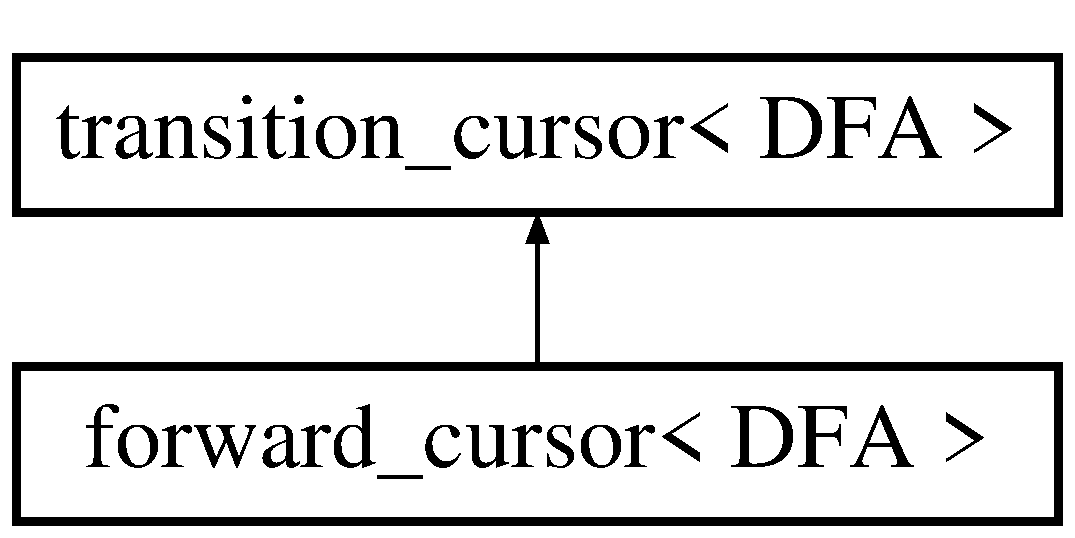
\includegraphics[height=2.000000cm]{classastl_1_1forward__cursor}
\end{center}
\end{figure}
\subsection*{Public Types}
\begin{DoxyCompactItemize}
\item 
typedef D\+F\+A\+::char\+\_\+traits {\bf char\+\_\+traits}\label{classastl_1_1forward__cursor_a6359447f7b84903df56c9979d803aa60}

\begin{DoxyCompactList}\small\item\em Character traits describing \doxyref{char\+\_\+type}{p.}{classastl_1_1forward__cursor_a6f0a01bfd199068ca92da76d90230cc5}. \end{DoxyCompactList}\item 
typedef D\+F\+A\+::char\+\_\+type {\bf char\+\_\+type}\label{classastl_1_1forward__cursor_a6f0a01bfd199068ca92da76d90230cc5}

\begin{DoxyCompactList}\small\item\em The type of the transitions letters. \end{DoxyCompactList}\item 
typedef D\+F\+A\+::state\+\_\+type {\bf state\+\_\+type}\label{classastl_1_1forward__cursor_a5688781e11c8c2c97986575ce50490d2}

\begin{DoxyCompactList}\small\item\em The type of the automaton-\/states identifiers. \end{DoxyCompactList}\item 
typedef D\+F\+A\+::tag\+\_\+type {\bf tag\+\_\+type}\label{classastl_1_1forward__cursor_a94f372c34a236e680045fd9067973591}

\begin{DoxyCompactList}\small\item\em The type of the data attached to states. \end{DoxyCompactList}\end{DoxyCompactItemize}
\subsection*{Public Member Functions}
\begin{DoxyCompactItemize}
\item 
{\bf state\+\_\+type} {\bf aim} () const
\begin{DoxyCompactList}\small\item\em Returns the aim state of the pointed transition. \end{DoxyCompactList}\item 
bool {\bf aim\+\_\+final} () const\label{classastl_1_1transition__cursor_a8fdf66e2483d23e73580e5c9ed937dfb}

\begin{DoxyCompactList}\small\item\em Returns {\ttfamily true} if the aim state of the transition that this cursor points to is final. \end{DoxyCompactList}\item 
const {\bf tag\+\_\+type} \& {\bf aim\+\_\+tag} () const\label{classastl_1_1transition__cursor_a6dae0fe9126450e9c463973e3414dbf0}

\begin{DoxyCompactList}\small\item\em Returns the data attached to the aim state of the pointed transition. \end{DoxyCompactList}\item 
bool {\bf exists} (const {\bf char\+\_\+type} \&a) const \label{classastl_1_1forward__cursor_a76881664fce15da44fe584dd40f5fe88}

\begin{DoxyCompactList}\small\item\em Returns {\ttfamily true} if an outgoing transition labeled with {\ttfamily a} exists. \end{DoxyCompactList}\item 
bool {\bf find} (const {\bf char\+\_\+type} \&a)
\begin{DoxyCompactList}\small\item\em Makes this cursor point to the transition labeled with {\ttfamily a}. \end{DoxyCompactList}\item 
bool {\bf first} ()
\begin{DoxyCompactList}\small\item\em Makes this cursor point to the first element of the transitions sequence of the source state. \end{DoxyCompactList}\item 
bool {\bf forward} (const {\bf char\+\_\+type} \&a)
\begin{DoxyCompactList}\small\item\em Moves along the outgoing transition labeled with {\ttfamily }. \end{DoxyCompactList}\item 
void {\bf forward} ()
\begin{DoxyCompactList}\small\item\em Moves forward along the pointed transition. \end{DoxyCompactList}\item 
{\bf forward\+\_\+cursor} (const D\+F\+A \&a, {\bf state\+\_\+type} p)\label{classastl_1_1forward__cursor_a4896d143c898646f9fccaaad9ec1ecd5}

\begin{DoxyCompactList}\small\item\em Creates a cursor pointing to a state {\ttfamily p} of the automaton {\ttfamily a}. \end{DoxyCompactList}\item 
{\bf forward\+\_\+cursor} (const D\+F\+A \&a)\label{classastl_1_1forward__cursor_aef777177af22ecfd347a213519ab0009}

\begin{DoxyCompactList}\small\item\em Creates a cursor pointing to an undefined state of the automaton {\ttfamily a}. \end{DoxyCompactList}\item 
{\bf forward\+\_\+cursor} ()\label{classastl_1_1forward__cursor_a617d3f33c2c4006bb9553c51ad123705}

\begin{DoxyCompactList}\small\item\em Creates a singular cursor. \end{DoxyCompactList}\item 
{\bf char\+\_\+type} {\bf letter} () const
\begin{DoxyCompactList}\small\item\em Returns the letter on the pointed transition. \end{DoxyCompactList}\item 
bool {\bf next} ()
\begin{DoxyCompactList}\small\item\em Moves this cursor to the next element of the transitions sequence of the source state. \end{DoxyCompactList}\item 
bool {\bf operator!=} (const {\bf self} \&x) const\label{classastl_1_1transition__cursor_aef9934be5de2e5c7dd83e1a6a71fd607}

\begin{DoxyCompactList}\small\item\em Returns {\ttfamily true} if {\ttfamily x} points to another transition than this cursor. \end{DoxyCompactList}\item 
{\bf self} \& {\bf operator=} ({\bf state\+\_\+type} p)
\begin{DoxyCompactList}\small\item\em Sets this cursor to point to the state {\ttfamily p}. \end{DoxyCompactList}\item 
bool {\bf operator==} (const {\bf self} \&x) const\label{classastl_1_1transition__cursor_a8a0948685b8eb65ce6775c8f12547439}

\begin{DoxyCompactList}\small\item\em Returns {\ttfamily true} if {\ttfamily x} points to the same transition as this cursor. \end{DoxyCompactList}\item 
bool {\bf sink} () const\label{classastl_1_1transition__cursor_aaa86c67665c4228704986fda795267b4}

\begin{DoxyCompactList}\small\item\em Returns {\ttfamily true} if this cursor points to the sink state {\ttfamily F\+A\+::null\+\_\+state}. \end{DoxyCompactList}\item 
{\bf state\+\_\+type} {\bf sink\+\_\+state} () const\label{classastl_1_1transition__cursor_a3d87af14424f9bc42682409b30c4861e}

\begin{DoxyCompactList}\small\item\em Returns the identifier of the sink state {\ttfamily F\+A\+::null\+\_\+state}. \end{DoxyCompactList}\item 
{\bf state\+\_\+type} {\bf src} () const\label{classastl_1_1transition__cursor_a137a201732fb341cc5972fe3781e50f0}

\begin{DoxyCompactList}\small\item\em Returns the id of the state that this cursor points to. \end{DoxyCompactList}\item 
bool {\bf src\+\_\+final} () const\label{classastl_1_1transition__cursor_adac68d94341c2d6f5005d3b21b823ff3}

\begin{DoxyCompactList}\small\item\em Returns {\ttfamily true} if the state this cursor points to is final. \end{DoxyCompactList}\item 
const {\bf tag\+\_\+type} \& {\bf src\+\_\+tag} () const\label{classastl_1_1transition__cursor_ad566703edb60ad110408084dc8d9fef2}

\begin{DoxyCompactList}\small\item\em Returns the data attached to the state this cursor points to. \end{DoxyCompactList}\end{DoxyCompactItemize}


\subsection{Detailed Description}
\subsubsection*{template$<$typename D\+F\+A$>$class astl\+::forward\+\_\+cursor$<$ D\+F\+A $>$}

A pointer to a deterministic-\/automaton transition ({\itshape source} {\itshape state}, {\itshape letter}, {\itshape aim} {\itshape state}). 

It provides all the functionnalities of the plain \#cursor and the \doxyref{transition\+\_\+cursor}{p.}{classastl_1_1transition__cursor_abed05cb242f7e3d4f12f243a45f68a78} \begin{DoxyParagraph}{Template parameters}
\begin{TabularC}{4}
\hline
\rowcolor{lightgray}{\bf Parameter}&{\bf Description}&{\bf Default}&{\bf Requirements }\\\cline{1-4}
{\ttfamily D\+F\+A} &The type of the automaton that this cursor will point to&&{\ttfamily D\+F\+A} is a model of \#\+D\+F\+A\\\cline{1-4}
\end{TabularC}

\end{DoxyParagraph}
\begin{DoxyParagraph}{Model of}
\#cursor, \doxyref{transition\+\_\+cursor}{p.}{classastl_1_1transition__cursor_abed05cb242f7e3d4f12f243a45f68a78}, \doxyref{forward\+\_\+cursor}{p.}{classastl_1_1forward__cursor_a4896d143c898646f9fccaaad9ec1ecd5} 
\end{DoxyParagraph}
\begin{DoxyParagraph}{Associated Helper Functions}
forwardc() 
\end{DoxyParagraph}


\subsection{Member Function Documentation}
\index{astl\+::forward\+\_\+cursor@{astl\+::forward\+\_\+cursor}!aim@{aim}}
\index{aim@{aim}!astl\+::forward\+\_\+cursor@{astl\+::forward\+\_\+cursor}}
\subsubsection[{aim}]{\setlength{\rightskip}{0pt plus 5cm}{\bf state\+\_\+type} aim (
\begin{DoxyParamCaption}
{}
\end{DoxyParamCaption}
) const\hspace{0.3cm}{\ttfamily [inherited]}}\label{classastl_1_1transition__cursor_a742bd0e539b1f9df56841304b7ef4272}


Returns the aim state of the pointed transition. 

\begin{DoxyPrecond}{Precondition}
The cursor shall have been set to point to a defined transition beforehand by successfully calling \doxyref{first}{p.}{classastl_1_1transition__cursor_ae9f7851f510732f6e146ce82bc44979e} or \doxyref{next}{p.}{classastl_1_1transition__cursor_a80870c233d0237e3588a2d6f8d176916} 
\end{DoxyPrecond}
\index{astl\+::forward\+\_\+cursor@{astl\+::forward\+\_\+cursor}!find@{find}}
\index{find@{find}!astl\+::forward\+\_\+cursor@{astl\+::forward\+\_\+cursor}}
\subsubsection[{find}]{\setlength{\rightskip}{0pt plus 5cm}bool find (
\begin{DoxyParamCaption}
\item[{const {\bf char\+\_\+type} \&}]{a}
\end{DoxyParamCaption}
)}\label{classastl_1_1forward__cursor_a01fb64a042e3a398a2cdac850416a6cd}


Makes this cursor point to the transition labeled with {\ttfamily a}. 

\begin{DoxyReturn}{Returns}
{\ttfamily true} if such a transition exists, otherwise return {\ttfamily false} and the pointed transition is undefined 
\end{DoxyReturn}
\index{astl\+::forward\+\_\+cursor@{astl\+::forward\+\_\+cursor}!first@{first}}
\index{first@{first}!astl\+::forward\+\_\+cursor@{astl\+::forward\+\_\+cursor}}
\subsubsection[{first}]{\setlength{\rightskip}{0pt plus 5cm}bool first (
\begin{DoxyParamCaption}
{}
\end{DoxyParamCaption}
)\hspace{0.3cm}{\ttfamily [inherited]}}\label{classastl_1_1transition__cursor_ae9f7851f510732f6e146ce82bc44979e}


Makes this cursor point to the first element of the transitions sequence of the source state. 

Returns {\ttfamily true} if such an element exists (if any transition is defined), otherwise the pointed transition is undefined \index{astl\+::forward\+\_\+cursor@{astl\+::forward\+\_\+cursor}!forward@{forward}}
\index{forward@{forward}!astl\+::forward\+\_\+cursor@{astl\+::forward\+\_\+cursor}}
\subsubsection[{forward}]{\setlength{\rightskip}{0pt plus 5cm}bool forward (
\begin{DoxyParamCaption}
\item[{const {\bf char\+\_\+type} \&}]{a}
\end{DoxyParamCaption}
)}\label{classastl_1_1forward__cursor_ac091f7bf62a33b9952934100cd13a2f4}


Moves along the outgoing transition labeled with {\ttfamily }. 

\begin{DoxyReturn}{Returns}
{\ttfamily true} if such a transition is defined, otherwise move to sink state and return {\ttfamily false} 
\end{DoxyReturn}
\index{astl\+::forward\+\_\+cursor@{astl\+::forward\+\_\+cursor}!forward@{forward}}
\index{forward@{forward}!astl\+::forward\+\_\+cursor@{astl\+::forward\+\_\+cursor}}
\subsubsection[{forward}]{\setlength{\rightskip}{0pt plus 5cm}void forward (
\begin{DoxyParamCaption}
{}
\end{DoxyParamCaption}
)}\label{classastl_1_1forward__cursor_a7de2a543986e45b9083c69f6138bf079}


Moves forward along the pointed transition. 

\begin{DoxyPrecond}{Precondition}
The cursor shall have been set to point to a defined transition beforehand by successfully calling \doxyref{first}{p.}{classastl_1_1transition__cursor_ae9f7851f510732f6e146ce82bc44979e}, \doxyref{next}{p.}{classastl_1_1transition__cursor_a80870c233d0237e3588a2d6f8d176916} or \doxyref{find}{p.}{classastl_1_1forward__cursor_a01fb64a042e3a398a2cdac850416a6cd} 
\end{DoxyPrecond}
\index{astl\+::forward\+\_\+cursor@{astl\+::forward\+\_\+cursor}!letter@{letter}}
\index{letter@{letter}!astl\+::forward\+\_\+cursor@{astl\+::forward\+\_\+cursor}}
\subsubsection[{letter}]{\setlength{\rightskip}{0pt plus 5cm}{\bf char\+\_\+type} letter (
\begin{DoxyParamCaption}
{}
\end{DoxyParamCaption}
) const\hspace{0.3cm}{\ttfamily [inherited]}}\label{classastl_1_1transition__cursor_a6b28dc14fee32fdbd1e558b9c4884c9f}


Returns the letter on the pointed transition. 

\begin{DoxyPrecond}{Precondition}
The cursor shall have been set to point to a defined transition beforehand by successfully calling \doxyref{first}{p.}{classastl_1_1transition__cursor_ae9f7851f510732f6e146ce82bc44979e} or \doxyref{next}{p.}{classastl_1_1transition__cursor_a80870c233d0237e3588a2d6f8d176916} 
\end{DoxyPrecond}
\index{astl\+::forward\+\_\+cursor@{astl\+::forward\+\_\+cursor}!next@{next}}
\index{next@{next}!astl\+::forward\+\_\+cursor@{astl\+::forward\+\_\+cursor}}
\subsubsection[{next}]{\setlength{\rightskip}{0pt plus 5cm}bool next (
\begin{DoxyParamCaption}
{}
\end{DoxyParamCaption}
)\hspace{0.3cm}{\ttfamily [inherited]}}\label{classastl_1_1transition__cursor_a80870c233d0237e3588a2d6f8d176916}


Moves this cursor to the next element of the transitions sequence of the source state. 

Returns {\ttfamily true} if such an element exists (the cursor is not at the end of the sequence), otherwise the pointed transition is undefined. \begin{DoxyPrecond}{Precondition}
The cursor shall have been set to point to a defined transition beforehand by successfully calling \doxyref{first}{p.}{classastl_1_1transition__cursor_ae9f7851f510732f6e146ce82bc44979e} or \doxyref{next}{p.}{classastl_1_1transition__cursor_a80870c233d0237e3588a2d6f8d176916} 
\end{DoxyPrecond}
\index{astl\+::forward\+\_\+cursor@{astl\+::forward\+\_\+cursor}!operator=@{operator=}}
\index{operator=@{operator=}!astl\+::forward\+\_\+cursor@{astl\+::forward\+\_\+cursor}}
\subsubsection[{operator=}]{\setlength{\rightskip}{0pt plus 5cm}{\bf self}\& operator= (
\begin{DoxyParamCaption}
\item[{{\bf state\+\_\+type}}]{p}
\end{DoxyParamCaption}
)}\label{classastl_1_1forward__cursor_af2636a625f63fd707ee326cd3149dc48}


Sets this cursor to point to the state {\ttfamily p}. 

\begin{DoxyPostcond}{Postcondition}

\begin{DoxyCode}
src() == p 
\end{DoxyCode}
 
\end{DoxyPostcond}

\section{forward\+\_\+dcursor$<$ N\+F\+A, Tag\+Mapper $>$ Class Template Reference}
\label{classastl_1_1forward__dcursor}\index{forward\+\_\+dcursor$<$ N\+F\+A, Tag\+Mapper $>$@{forward\+\_\+dcursor$<$ N\+F\+A, Tag\+Mapper $>$}}


A forward cursor to a non-\/deterministic automaton computing the determinization on-\/the-\/fly.  




{\ttfamily \#include $<$determinize.\+h$>$}

Inheritance diagram for forward\+\_\+dcursor$<$ N\+F\+A, Tag\+Mapper $>$\+:\begin{figure}[H]
\begin{center}
\leavevmode
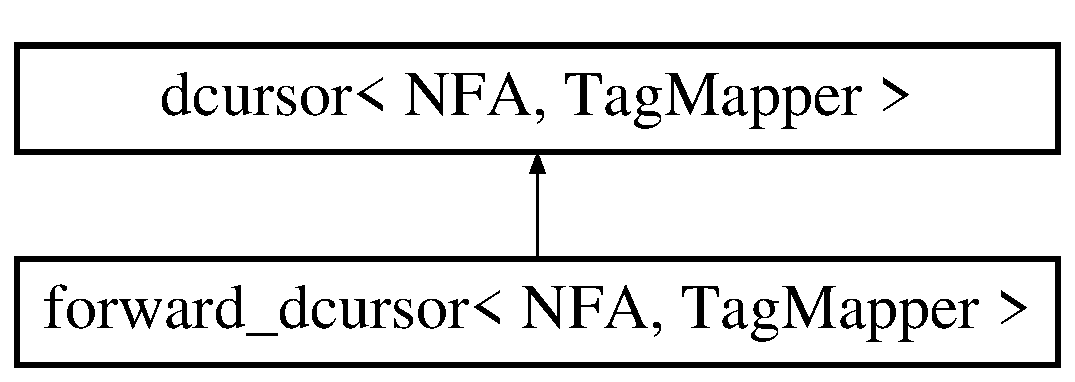
\includegraphics[height=2.000000cm]{classastl_1_1forward__dcursor}
\end{center}
\end{figure}


\subsection{Detailed Description}
\subsubsection*{template$<$typename N\+F\+A, typename Tag\+Mapper = default\+\_\+tag\+\_\+mapper$<$\+N\+F\+A$>$$>$class astl\+::forward\+\_\+dcursor$<$ N\+F\+A, Tag\+Mapper $>$}

A forward cursor to a non-\/deterministic automaton computing the determinization on-\/the-\/fly. 

\begin{DoxyParagraph}{Associated Helper Functions}
\#forwarddc() 
\end{DoxyParagraph}

\section{queue\+\_\+cursor$<$ Forward\+Cursor, Queue\+Container $>$ Class Template Reference}
\label{classastl_1_1queue__cursor}\index{queue\+\_\+cursor$<$ Forward\+Cursor, Queue\+Container $>$@{queue\+\_\+cursor$<$ Forward\+Cursor, Queue\+Container $>$}}


A \#forward\+\_\+cursor storing its path in a queue of cursors.  




{\ttfamily \#include $<$cursor.\+h$>$}



Inherits Queue\+Container, and queue\+\_\+cursor\+\_\+concept.

\subsection*{Public Types}
\begin{DoxyCompactItemize}
\item 
typedef Forward\+Cursor\+::char\+\_\+traits {\bf char\+\_\+traits}\label{classastl_1_1queue__cursor_ad8bde426782829974765ca3cf9e55e88}

\begin{DoxyCompactList}\small\item\em Character traits describing \doxyref{char\+\_\+type}{p.}{classastl_1_1queue__cursor_abca675437fcd5cc259bc0a9ff8ca5846}. \end{DoxyCompactList}\item 
typedef Forward\+Cursor\+::char\+\_\+type {\bf char\+\_\+type}\label{classastl_1_1queue__cursor_abca675437fcd5cc259bc0a9ff8ca5846}

\begin{DoxyCompactList}\small\item\em The type of the transitions letters. \end{DoxyCompactList}\item 
typedef Forward\+Cursor\+::state\+\_\+type {\bf state\+\_\+type}\label{classastl_1_1queue__cursor_a40cdabeccae4cfdf971eb6593bdd602e}

\begin{DoxyCompactList}\small\item\em The type of the automaton-\/states identifiers. \end{DoxyCompactList}\item 
typedef Forward\+Cursor\+::tag\+\_\+type {\bf tag\+\_\+type}\label{classastl_1_1queue__cursor_a865d5f4253e69bee2ab7fff1cbcce2d0}

\begin{DoxyCompactList}\small\item\em The type of the data attached to states. \end{DoxyCompactList}\end{DoxyCompactItemize}
\subsection*{Public Member Functions}
\begin{DoxyCompactItemize}
\item 
{\bf state\+\_\+type} {\bf aim} () const 
\begin{DoxyCompactList}\small\item\em Returns the aim state of the pointed transition. \end{DoxyCompactList}\item 
bool {\bf aim\+\_\+final} () const 
\begin{DoxyCompactList}\small\item\em Returns {\ttfamily true} if the aim state of the transition that this cursor points to is final. \end{DoxyCompactList}\item 
{\bf tag\+\_\+type} {\bf aim\+\_\+tag} () const 
\begin{DoxyCompactList}\small\item\em Returns the data attached to the aim state of the pointed transition. \end{DoxyCompactList}\item 
bool {\bf dequeue} ()
\begin{DoxyCompactList}\small\item\em Dequeues a forward cursor and return {\ttfamily false} if the resulting queue is empty. \end{DoxyCompactList}\item 
bool {\bf exists} (const {\bf char\+\_\+type} \&a) const 
\begin{DoxyCompactList}\small\item\em Returns {\ttfamily true} if an outgoing transition labeled with {\ttfamily a} exists. \end{DoxyCompactList}\item 
bool {\bf find} (const {\bf char\+\_\+type} \&a)\label{classastl_1_1queue__cursor_a01fb64a042e3a398a2cdac850416a6cd}

\begin{DoxyCompactList}\small\item\em Returns the sink state identifier. \end{DoxyCompactList}\item 
bool {\bf first} ()
\begin{DoxyCompactList}\small\item\em Makes this cursor point to the first element of the transitions sequence of the source state and enqueues the resulting forward cursor. \end{DoxyCompactList}\item 
void {\bf forward} ()
\begin{DoxyCompactList}\small\item\em Moves forward along the pointed transition. \end{DoxyCompactList}\item 
bool {\bf forward} (const {\bf char\+\_\+type} \&a)
\begin{DoxyCompactList}\small\item\em Moves along the outgoing transition labeled with {\ttfamily a} if defined, otherwise moves to sink state and returns {\ttfamily false}. \end{DoxyCompactList}\item 
{\bf char\+\_\+type} {\bf letter} () const 
\begin{DoxyCompactList}\small\item\em Returns the letter on the pointed transition. \end{DoxyCompactList}\item 
bool {\bf next} ()
\begin{DoxyCompactList}\small\item\em Moves this cursor to the next element of the transitions sequence of the source state and enqueues the resulting cursor. \end{DoxyCompactList}\item 
{\bf queue\+\_\+cursor} (const Forward\+Cursor \&x)\label{classastl_1_1queue__cursor_a3eb87e41e8868cb16e6ce3b78ed6bfb4}

\begin{DoxyCompactList}\small\item\em Creates a cursor with a queue containing {\ttfamily x}. \end{DoxyCompactList}\item 
{\bf queue\+\_\+cursor} ()\label{classastl_1_1queue__cursor_a22cb0e5eafb62b8ddf7190ece228fcc6}

\begin{DoxyCompactList}\small\item\em Creates a cursor with an empty queue. \end{DoxyCompactList}\item 
bool {\bf sink} () const 
\begin{DoxyCompactList}\small\item\em Returns {\ttfamily true} if this cursor points to the sink state. \end{DoxyCompactList}\item 
{\bf state\+\_\+type} {\bf src} () const 
\begin{DoxyCompactList}\small\item\em Returns the identifier of the state that this cursor points to. \end{DoxyCompactList}\item 
bool {\bf src\+\_\+final} () const 
\begin{DoxyCompactList}\small\item\em Returns {\ttfamily true} if the state that this cursor points to is final. \end{DoxyCompactList}\item 
{\bf tag\+\_\+type} {\bf src\+\_\+tag} () const 
\begin{DoxyCompactList}\small\item\em Returns the data attached to the state that this cursor points to. \end{DoxyCompactList}\end{DoxyCompactItemize}


\subsection{Detailed Description}
\subsubsection*{template$<$typename Forward\+Cursor, typename Queue\+Container = deque$<$\+Forward\+Cursor$>$$>$class astl\+::queue\+\_\+cursor$<$ Forward\+Cursor, Queue\+Container $>$}

A \#forward\+\_\+cursor storing its path in a queue of cursors. 

Each move through the sequence of the outgoing transitions of the source state (\doxyref{next()}{p.}{classastl_1_1queue__cursor_a80870c233d0237e3588a2d6f8d176916}) enqueues a forward cursor. An extra method \doxyref{dequeue()}{p.}{classastl_1_1queue__cursor_a251b7c8fd6f9441d6a96a70fcc83e30a} allows to dequeue and to implement the breadth-\/first traversal. \begin{DoxyParagraph}{Template parameters}
\begin{TabularC}{4}
\hline
\rowcolor{lightgray}{\bf Parameter}&{\bf Description}&{\bf Default}&{\bf Requirements }\\\cline{1-4}
{\ttfamily Forward\+Cursor} &The type of the cursors that are stored in the queue&&{\ttfamily Forward\+Cursor} is a model of forward cursor \\\cline{1-4}
{\ttfamily Queue\+Container} &The type of the sequential container managing the queue&{\ttfamily deque$<$\+Forward\+Cursor$>$} &{\ttfamily Queue\+Container} is a model of front and back insertion sequence and {\ttfamily Queue\+Container\+::value\+\_\+type} is {\ttfamily Forward\+Cursor} \\\cline{1-4}
\end{TabularC}

\end{DoxyParagraph}
\begin{DoxyParagraph}{Model of}
cursor, transition cursor, forward cursor, queue cursor 
\end{DoxyParagraph}
\begin{DoxyParagraph}{Associated Helper Functions}
queuec() 
\end{DoxyParagraph}


\subsection{Member Function Documentation}
\index{astl\+::queue\+\_\+cursor@{astl\+::queue\+\_\+cursor}!aim@{aim}}
\index{aim@{aim}!astl\+::queue\+\_\+cursor@{astl\+::queue\+\_\+cursor}}
\subsubsection[{aim}]{\setlength{\rightskip}{0pt plus 5cm}{\bf state\+\_\+type} aim (
\begin{DoxyParamCaption}
{}
\end{DoxyParamCaption}
) const}\label{classastl_1_1queue__cursor_a742bd0e539b1f9df56841304b7ef4272}


Returns the aim state of the pointed transition. 

\begin{DoxyPrecond}{Precondition}
The queue is not empty. 

The cursor shall have been set to point to a defined transition beforehand by successfully calling \doxyref{first}{p.}{classastl_1_1queue__cursor_ae9f7851f510732f6e146ce82bc44979e}, \doxyref{next}{p.}{classastl_1_1queue__cursor_a80870c233d0237e3588a2d6f8d176916} or \doxyref{find}{p.}{classastl_1_1queue__cursor_a01fb64a042e3a398a2cdac850416a6cd} 
\end{DoxyPrecond}
\index{astl\+::queue\+\_\+cursor@{astl\+::queue\+\_\+cursor}!aim\+\_\+final@{aim\+\_\+final}}
\index{aim\+\_\+final@{aim\+\_\+final}!astl\+::queue\+\_\+cursor@{astl\+::queue\+\_\+cursor}}
\subsubsection[{aim\+\_\+final}]{\setlength{\rightskip}{0pt plus 5cm}bool aim\+\_\+final (
\begin{DoxyParamCaption}
{}
\end{DoxyParamCaption}
) const}\label{classastl_1_1queue__cursor_a8fdf66e2483d23e73580e5c9ed937dfb}


Returns {\ttfamily true} if the aim state of the transition that this cursor points to is final. 

\begin{DoxyPrecond}{Precondition}
The queue is not empty 
\end{DoxyPrecond}
\index{astl\+::queue\+\_\+cursor@{astl\+::queue\+\_\+cursor}!aim\+\_\+tag@{aim\+\_\+tag}}
\index{aim\+\_\+tag@{aim\+\_\+tag}!astl\+::queue\+\_\+cursor@{astl\+::queue\+\_\+cursor}}
\subsubsection[{aim\+\_\+tag}]{\setlength{\rightskip}{0pt plus 5cm}{\bf tag\+\_\+type} aim\+\_\+tag (
\begin{DoxyParamCaption}
{}
\end{DoxyParamCaption}
) const}\label{classastl_1_1queue__cursor_a76a01210687f95ea151f8073a0eac35f}


Returns the data attached to the aim state of the pointed transition. 

\begin{DoxyPrecond}{Precondition}
The queue is not empty. 
\end{DoxyPrecond}
\index{astl\+::queue\+\_\+cursor@{astl\+::queue\+\_\+cursor}!dequeue@{dequeue}}
\index{dequeue@{dequeue}!astl\+::queue\+\_\+cursor@{astl\+::queue\+\_\+cursor}}
\subsubsection[{dequeue}]{\setlength{\rightskip}{0pt plus 5cm}bool dequeue (
\begin{DoxyParamCaption}
{}
\end{DoxyParamCaption}
)}\label{classastl_1_1queue__cursor_a251b7c8fd6f9441d6a96a70fcc83e30a}


Dequeues a forward cursor and return {\ttfamily false} if the resulting queue is empty. 

\begin{DoxyPrecond}{Precondition}
The queue is not empty 
\end{DoxyPrecond}
\index{astl\+::queue\+\_\+cursor@{astl\+::queue\+\_\+cursor}!exists@{exists}}
\index{exists@{exists}!astl\+::queue\+\_\+cursor@{astl\+::queue\+\_\+cursor}}
\subsubsection[{exists}]{\setlength{\rightskip}{0pt plus 5cm}bool exists (
\begin{DoxyParamCaption}
\item[{const {\bf char\+\_\+type} \&}]{a}
\end{DoxyParamCaption}
) const}\label{classastl_1_1queue__cursor_a76881664fce15da44fe584dd40f5fe88}


Returns {\ttfamily true} if an outgoing transition labeled with {\ttfamily a} exists. 

\begin{DoxyPrecond}{Precondition}
The queue is not empty 
\end{DoxyPrecond}
\index{astl\+::queue\+\_\+cursor@{astl\+::queue\+\_\+cursor}!first@{first}}
\index{first@{first}!astl\+::queue\+\_\+cursor@{astl\+::queue\+\_\+cursor}}
\subsubsection[{first}]{\setlength{\rightskip}{0pt plus 5cm}bool first (
\begin{DoxyParamCaption}
{}
\end{DoxyParamCaption}
)}\label{classastl_1_1queue__cursor_ae9f7851f510732f6e146ce82bc44979e}


Makes this cursor point to the first element of the transitions sequence of the source state and enqueues the resulting forward cursor. 

Returns {\ttfamily true} if such an element exists (if any transition is defined), otherwise the pointed transition is undefined. \begin{DoxyPrecond}{Precondition}
The queue is not empty 
\end{DoxyPrecond}
\index{astl\+::queue\+\_\+cursor@{astl\+::queue\+\_\+cursor}!forward@{forward}}
\index{forward@{forward}!astl\+::queue\+\_\+cursor@{astl\+::queue\+\_\+cursor}}
\subsubsection[{forward}]{\setlength{\rightskip}{0pt plus 5cm}void forward (
\begin{DoxyParamCaption}
{}
\end{DoxyParamCaption}
)}\label{classastl_1_1queue__cursor_a7de2a543986e45b9083c69f6138bf079}


Moves forward along the pointed transition. 

\begin{DoxyPrecond}{Precondition}
The queue is not empty. 

The cursor shall have been set to point to a defined transition beforehand by successfully calling \doxyref{first}{p.}{classastl_1_1queue__cursor_ae9f7851f510732f6e146ce82bc44979e}, \doxyref{next}{p.}{classastl_1_1queue__cursor_a80870c233d0237e3588a2d6f8d176916} or \doxyref{find}{p.}{classastl_1_1queue__cursor_a01fb64a042e3a398a2cdac850416a6cd} 
\end{DoxyPrecond}
\index{astl\+::queue\+\_\+cursor@{astl\+::queue\+\_\+cursor}!forward@{forward}}
\index{forward@{forward}!astl\+::queue\+\_\+cursor@{astl\+::queue\+\_\+cursor}}
\subsubsection[{forward}]{\setlength{\rightskip}{0pt plus 5cm}bool forward (
\begin{DoxyParamCaption}
\item[{const {\bf char\+\_\+type} \&}]{a}
\end{DoxyParamCaption}
)}\label{classastl_1_1queue__cursor_ac091f7bf62a33b9952934100cd13a2f4}


Moves along the outgoing transition labeled with {\ttfamily a} if defined, otherwise moves to sink state and returns {\ttfamily false}. 

\begin{DoxyPrecond}{Precondition}
The queue is not empty 
\end{DoxyPrecond}
\index{astl\+::queue\+\_\+cursor@{astl\+::queue\+\_\+cursor}!letter@{letter}}
\index{letter@{letter}!astl\+::queue\+\_\+cursor@{astl\+::queue\+\_\+cursor}}
\subsubsection[{letter}]{\setlength{\rightskip}{0pt plus 5cm}{\bf char\+\_\+type} letter (
\begin{DoxyParamCaption}
{}
\end{DoxyParamCaption}
) const}\label{classastl_1_1queue__cursor_a6b28dc14fee32fdbd1e558b9c4884c9f}


Returns the letter on the pointed transition. 

. \begin{DoxyPrecond}{Precondition}
The queue is not empty. 

The cursor shall have been set to point to a defined transition beforehand by successfully calling \doxyref{first}{p.}{classastl_1_1queue__cursor_ae9f7851f510732f6e146ce82bc44979e}, \doxyref{next}{p.}{classastl_1_1queue__cursor_a80870c233d0237e3588a2d6f8d176916} or \doxyref{find}{p.}{classastl_1_1queue__cursor_a01fb64a042e3a398a2cdac850416a6cd} 
\end{DoxyPrecond}
\index{astl\+::queue\+\_\+cursor@{astl\+::queue\+\_\+cursor}!next@{next}}
\index{next@{next}!astl\+::queue\+\_\+cursor@{astl\+::queue\+\_\+cursor}}
\subsubsection[{next}]{\setlength{\rightskip}{0pt plus 5cm}bool next (
\begin{DoxyParamCaption}
{}
\end{DoxyParamCaption}
)}\label{classastl_1_1queue__cursor_a80870c233d0237e3588a2d6f8d176916}


Moves this cursor to the next element of the transitions sequence of the source state and enqueues the resulting cursor. 

Returns {\ttfamily true} if such an element exists (the cursor is not at the end of the sequence), otherwise dequeues a forward cursor and returns {\ttfamily false}. \begin{DoxyPrecond}{Precondition}
The queue is not empty. 

The cursor shall have been set to point to a defined transition beforehand by successfully calling \doxyref{first}{p.}{classastl_1_1queue__cursor_ae9f7851f510732f6e146ce82bc44979e}, \doxyref{next}{p.}{classastl_1_1queue__cursor_a80870c233d0237e3588a2d6f8d176916} or \doxyref{find}{p.}{classastl_1_1queue__cursor_a01fb64a042e3a398a2cdac850416a6cd} 
\end{DoxyPrecond}
\index{astl\+::queue\+\_\+cursor@{astl\+::queue\+\_\+cursor}!sink@{sink}}
\index{sink@{sink}!astl\+::queue\+\_\+cursor@{astl\+::queue\+\_\+cursor}}
\subsubsection[{sink}]{\setlength{\rightskip}{0pt plus 5cm}bool sink (
\begin{DoxyParamCaption}
{}
\end{DoxyParamCaption}
) const}\label{classastl_1_1queue__cursor_aaa86c67665c4228704986fda795267b4}


Returns {\ttfamily true} if this cursor points to the sink state. 

\begin{DoxyPrecond}{Precondition}
The queue is not empty 
\end{DoxyPrecond}
\index{astl\+::queue\+\_\+cursor@{astl\+::queue\+\_\+cursor}!src@{src}}
\index{src@{src}!astl\+::queue\+\_\+cursor@{astl\+::queue\+\_\+cursor}}
\subsubsection[{src}]{\setlength{\rightskip}{0pt plus 5cm}{\bf state\+\_\+type} src (
\begin{DoxyParamCaption}
{}
\end{DoxyParamCaption}
) const}\label{classastl_1_1queue__cursor_a137a201732fb341cc5972fe3781e50f0}


Returns the identifier of the state that this cursor points to. 

\begin{DoxyPrecond}{Precondition}
The queue is not empty 
\end{DoxyPrecond}
\index{astl\+::queue\+\_\+cursor@{astl\+::queue\+\_\+cursor}!src\+\_\+final@{src\+\_\+final}}
\index{src\+\_\+final@{src\+\_\+final}!astl\+::queue\+\_\+cursor@{astl\+::queue\+\_\+cursor}}
\subsubsection[{src\+\_\+final}]{\setlength{\rightskip}{0pt plus 5cm}bool src\+\_\+final (
\begin{DoxyParamCaption}
{}
\end{DoxyParamCaption}
) const}\label{classastl_1_1queue__cursor_adac68d94341c2d6f5005d3b21b823ff3}


Returns {\ttfamily true} if the state that this cursor points to is final. 

\begin{DoxyPrecond}{Precondition}
The queue is not empty 
\end{DoxyPrecond}
\index{astl\+::queue\+\_\+cursor@{astl\+::queue\+\_\+cursor}!src\+\_\+tag@{src\+\_\+tag}}
\index{src\+\_\+tag@{src\+\_\+tag}!astl\+::queue\+\_\+cursor@{astl\+::queue\+\_\+cursor}}
\subsubsection[{src\+\_\+tag}]{\setlength{\rightskip}{0pt plus 5cm}{\bf tag\+\_\+type} src\+\_\+tag (
\begin{DoxyParamCaption}
{}
\end{DoxyParamCaption}
) const}\label{classastl_1_1queue__cursor_a530bf00de29674ef6743b3375d5732f5}


Returns the data attached to the state that this cursor points to. 

\begin{DoxyPrecond}{Precondition}
The queue is not empty. 
\end{DoxyPrecond}

\section{stack\+\_\+cursor$<$ Forward\+Cursor, Stack\+Container $>$ Class Template Reference}
\label{classastl_1_1stack__cursor}\index{stack\+\_\+cursor$<$ Forward\+Cursor, Stack\+Container $>$@{stack\+\_\+cursor$<$ Forward\+Cursor, Stack\+Container $>$}}


A \#forward\+\_\+cursor storing its path in a stack of cursors.  




{\ttfamily \#include $<$cursor.\+h$>$}



Inherits Stack\+Container, and stack\+\_\+cursor\+\_\+concept.

\subsection*{Public Types}
\begin{DoxyCompactItemize}
\item 
typedef Forward\+Cursor\+::char\+\_\+traits {\bf char\+\_\+traits}\label{classastl_1_1stack__cursor_ad8bde426782829974765ca3cf9e55e88}

\begin{DoxyCompactList}\small\item\em Character traits describing \doxyref{char\+\_\+type}{p.}{classastl_1_1stack__cursor_abca675437fcd5cc259bc0a9ff8ca5846}. \end{DoxyCompactList}\item 
typedef Forward\+Cursor\+::char\+\_\+type {\bf char\+\_\+type}\label{classastl_1_1stack__cursor_abca675437fcd5cc259bc0a9ff8ca5846}

\begin{DoxyCompactList}\small\item\em The type of the transitions letters. \end{DoxyCompactList}\item 
typedef Forward\+Cursor\+::state\+\_\+type {\bf state\+\_\+type}\label{classastl_1_1stack__cursor_a40cdabeccae4cfdf971eb6593bdd602e}

\begin{DoxyCompactList}\small\item\em The type of the automaton-\/states identifiers. \end{DoxyCompactList}\item 
typedef Forward\+Cursor\+::tag\+\_\+type {\bf tag\+\_\+type}\label{classastl_1_1stack__cursor_a865d5f4253e69bee2ab7fff1cbcce2d0}

\begin{DoxyCompactList}\small\item\em The type of the data attached to states. \end{DoxyCompactList}\end{DoxyCompactItemize}
\subsection*{Public Member Functions}
\begin{DoxyCompactItemize}
\item 
{\bf state\+\_\+type} {\bf aim} () const 
\begin{DoxyCompactList}\small\item\em Returns the aim state of the pointed transition. \end{DoxyCompactList}\item 
bool {\bf aim\+\_\+final} () const 
\begin{DoxyCompactList}\small\item\em Returns {\ttfamily true} if the aim state of the transition that this cursor points to is final. \end{DoxyCompactList}\item 
{\bf tag\+\_\+type} {\bf aim\+\_\+tag} () const 
\begin{DoxyCompactList}\small\item\em Returns the data attached to the aim state of the pointed transition. \end{DoxyCompactList}\item 
bool {\bf backward} ()
\begin{DoxyCompactList}\small\item\em Pops the stack top and return {\ttfamily false} if the resulting stack is empty. \end{DoxyCompactList}\item 
bool {\bf exists} (const {\bf char\+\_\+type} \&a) const 
\begin{DoxyCompactList}\small\item\em Returns {\ttfamily true} if an outgoing transition labeled with {\ttfamily a} exists. \end{DoxyCompactList}\item 
bool {\bf find} (const {\bf char\+\_\+type} \&a)
\begin{DoxyCompactList}\small\item\em Makes this cursor point to the transition labeled with {\ttfamily a}. \end{DoxyCompactList}\item 
bool {\bf first} ()
\begin{DoxyCompactList}\small\item\em Makes this cursor point to the first element of the transitions sequence of the source state. \end{DoxyCompactList}\item 
void {\bf forward} ()
\begin{DoxyCompactList}\small\item\em Moves forward along the pointed transition and the resulting cursor is pushed onto the stack. \end{DoxyCompactList}\item 
bool {\bf forward} (const {\bf char\+\_\+type} \&a)
\begin{DoxyCompactList}\small\item\em Moves along the outgoing transition labeled with {\ttfamily a} if defined, otherwise moves to sink state and returns {\ttfamily false}. \end{DoxyCompactList}\item 
{\bf char\+\_\+type} {\bf letter} () const 
\begin{DoxyCompactList}\small\item\em Returns the letter on the pointed transition. \end{DoxyCompactList}\item 
bool {\bf next} ()
\begin{DoxyCompactList}\small\item\em Moves this cursor to the next element of the transitions sequence of the source state. \end{DoxyCompactList}\item 
bool {\bf sink} () const 
\begin{DoxyCompactList}\small\item\em Returns {\ttfamily true} if this cursor points to the sink state. \end{DoxyCompactList}\item 
{\bf state\+\_\+type} {\bf sink\+\_\+state} () const 
\begin{DoxyCompactList}\small\item\em Returns the sink state identifier. \end{DoxyCompactList}\item 
{\bf state\+\_\+type} {\bf src} () const 
\begin{DoxyCompactList}\small\item\em Returns the identifier of the state that this cursor points to. \end{DoxyCompactList}\item 
bool {\bf src\+\_\+final} () const 
\begin{DoxyCompactList}\small\item\em Returns {\ttfamily true} if the state that this cursor points to is final. \end{DoxyCompactList}\item 
{\bf tag\+\_\+type} {\bf src\+\_\+tag} () const 
\begin{DoxyCompactList}\small\item\em Returns the data attached to the state that this cursor points to. \end{DoxyCompactList}\item 
{\bf stack\+\_\+cursor} (const Forward\+Cursor \&x)\label{classastl_1_1stack__cursor_abe457749342fd1bf78860c966428035b}

\begin{DoxyCompactList}\small\item\em Creates a cursor with a stack containing {\ttfamily x}. \end{DoxyCompactList}\item 
{\bf stack\+\_\+cursor} ()\label{classastl_1_1stack__cursor_a66fe44763af97dded05e0af27444210b}

\begin{DoxyCompactList}\small\item\em Creates a cursor with an empty stack. \end{DoxyCompactList}\item 
const Forward\+Cursor \& {\bf top} () const 
\begin{DoxyCompactList}\small\item\em Returns the stack top. \end{DoxyCompactList}\end{DoxyCompactItemize}


\subsection{Detailed Description}
\subsubsection*{template$<$typename Forward\+Cursor, typename Stack\+Container = vector$<$\+Forward\+Cursor$>$$>$class astl\+::stack\+\_\+cursor$<$ Forward\+Cursor, Stack\+Container $>$}

A \#forward\+\_\+cursor storing its path in a stack of cursors. 

Each forward move along a transition pushes a new \#forward\+\_\+cursor onto the stack top and an extra method \doxyref{backward()}{p.}{classastl_1_1stack__cursor_ab861d77763d681d57e2ff48841e1f66f} allows to pop. The depth-\/first traversal cursor \#dfirst\+\_\+cursor relies on the \doxyref{stack\+\_\+cursor}{p.}{classastl_1_1stack__cursor_abe457749342fd1bf78860c966428035b} \begin{DoxyParagraph}{Template parameters}
\begin{TabularC}{4}
\hline
\rowcolor{lightgray}{\bf Parameter}&{\bf Description}&{\bf Default}&{\bf Requirements }\\\cline{1-4}
{\ttfamily Forward\+Cursor} &The type of the cursors that are stored on the stack&&{\ttfamily Forward\+Cursor} is a model of forward cursor \\\cline{1-4}
{\ttfamily Stack\+Container} &The type of the sequential container managing the stack&{\ttfamily vector$<$\+Forward\+Cursor$>$} &{\ttfamily Stack\+Container} is a model of back insertion sequence and {\ttfamily Stack\+Container\+::value\+\_\+type} is {\ttfamily Forward\+Cursor} \\\cline{1-4}
\end{TabularC}

\end{DoxyParagraph}
\begin{DoxyParagraph}{Model of}
cursor, transition cursor, forward cursor, stack cursor 
\end{DoxyParagraph}
\begin{DoxyParagraph}{Associated Helper Functions}
stackc() 
\end{DoxyParagraph}


\subsection{Member Function Documentation}
\index{astl\+::stack\+\_\+cursor@{astl\+::stack\+\_\+cursor}!aim@{aim}}
\index{aim@{aim}!astl\+::stack\+\_\+cursor@{astl\+::stack\+\_\+cursor}}
\subsubsection[{aim}]{\setlength{\rightskip}{0pt plus 5cm}{\bf state\+\_\+type} aim (
\begin{DoxyParamCaption}
{}
\end{DoxyParamCaption}
) const}\label{classastl_1_1stack__cursor_a742bd0e539b1f9df56841304b7ef4272}


Returns the aim state of the pointed transition. 

\begin{DoxyPrecond}{Precondition}
The stack is not empty. 

The cursor shall have been set to point to a defined transition beforehand by successfully calling \doxyref{first}{p.}{classastl_1_1stack__cursor_ae9f7851f510732f6e146ce82bc44979e}, \doxyref{next}{p.}{classastl_1_1stack__cursor_a80870c233d0237e3588a2d6f8d176916} or \doxyref{find}{p.}{classastl_1_1stack__cursor_a01fb64a042e3a398a2cdac850416a6cd} 
\end{DoxyPrecond}


Referenced by D\+F\+A\+\_\+min\+\_\+hash$<$ Char\+Traits $>$\+::insert().

\index{astl\+::stack\+\_\+cursor@{astl\+::stack\+\_\+cursor}!aim\+\_\+final@{aim\+\_\+final}}
\index{aim\+\_\+final@{aim\+\_\+final}!astl\+::stack\+\_\+cursor@{astl\+::stack\+\_\+cursor}}
\subsubsection[{aim\+\_\+final}]{\setlength{\rightskip}{0pt plus 5cm}bool aim\+\_\+final (
\begin{DoxyParamCaption}
{}
\end{DoxyParamCaption}
) const}\label{classastl_1_1stack__cursor_a8fdf66e2483d23e73580e5c9ed937dfb}


Returns {\ttfamily true} if the aim state of the transition that this cursor points to is final. 

\begin{DoxyPrecond}{Precondition}
The stack is not empty. 
\end{DoxyPrecond}
\index{astl\+::stack\+\_\+cursor@{astl\+::stack\+\_\+cursor}!aim\+\_\+tag@{aim\+\_\+tag}}
\index{aim\+\_\+tag@{aim\+\_\+tag}!astl\+::stack\+\_\+cursor@{astl\+::stack\+\_\+cursor}}
\subsubsection[{aim\+\_\+tag}]{\setlength{\rightskip}{0pt plus 5cm}{\bf tag\+\_\+type} aim\+\_\+tag (
\begin{DoxyParamCaption}
{}
\end{DoxyParamCaption}
) const}\label{classastl_1_1stack__cursor_a76a01210687f95ea151f8073a0eac35f}


Returns the data attached to the aim state of the pointed transition. 

\begin{DoxyPrecond}{Precondition}
The stack is not empty. 
\end{DoxyPrecond}
\index{astl\+::stack\+\_\+cursor@{astl\+::stack\+\_\+cursor}!backward@{backward}}
\index{backward@{backward}!astl\+::stack\+\_\+cursor@{astl\+::stack\+\_\+cursor}}
\subsubsection[{backward}]{\setlength{\rightskip}{0pt plus 5cm}bool backward (
\begin{DoxyParamCaption}
{}
\end{DoxyParamCaption}
)}\label{classastl_1_1stack__cursor_ab861d77763d681d57e2ff48841e1f66f}


Pops the stack top and return {\ttfamily false} if the resulting stack is empty. 

\begin{DoxyPrecond}{Precondition}
The stack is not empty 
\end{DoxyPrecond}


Referenced by D\+F\+A\+\_\+min\+\_\+hash$<$ Char\+Traits $>$\+::insert().

\index{astl\+::stack\+\_\+cursor@{astl\+::stack\+\_\+cursor}!exists@{exists}}
\index{exists@{exists}!astl\+::stack\+\_\+cursor@{astl\+::stack\+\_\+cursor}}
\subsubsection[{exists}]{\setlength{\rightskip}{0pt plus 5cm}bool exists (
\begin{DoxyParamCaption}
\item[{const {\bf char\+\_\+type} \&}]{a}
\end{DoxyParamCaption}
) const}\label{classastl_1_1stack__cursor_a76881664fce15da44fe584dd40f5fe88}


Returns {\ttfamily true} if an outgoing transition labeled with {\ttfamily a} exists. 

\begin{DoxyPrecond}{Precondition}
The stack is not empty 
\end{DoxyPrecond}
\index{astl\+::stack\+\_\+cursor@{astl\+::stack\+\_\+cursor}!find@{find}}
\index{find@{find}!astl\+::stack\+\_\+cursor@{astl\+::stack\+\_\+cursor}}
\subsubsection[{find}]{\setlength{\rightskip}{0pt plus 5cm}bool find (
\begin{DoxyParamCaption}
\item[{const {\bf char\+\_\+type} \&}]{a}
\end{DoxyParamCaption}
)}\label{classastl_1_1stack__cursor_a01fb64a042e3a398a2cdac850416a6cd}


Makes this cursor point to the transition labeled with {\ttfamily a}. 

Returns {\ttfamily true} if such a transition exists, otherwise the pointed transition is undefined. \begin{DoxyPrecond}{Precondition}
The stack is not empty 
\end{DoxyPrecond}


Referenced by D\+F\+A\+\_\+min\+\_\+hash$<$ Char\+Traits $>$\+::insert().

\index{astl\+::stack\+\_\+cursor@{astl\+::stack\+\_\+cursor}!first@{first}}
\index{first@{first}!astl\+::stack\+\_\+cursor@{astl\+::stack\+\_\+cursor}}
\subsubsection[{first}]{\setlength{\rightskip}{0pt plus 5cm}bool first (
\begin{DoxyParamCaption}
{}
\end{DoxyParamCaption}
)}\label{classastl_1_1stack__cursor_ae9f7851f510732f6e146ce82bc44979e}


Makes this cursor point to the first element of the transitions sequence of the source state. 

Returns {\ttfamily true} if such an element exists (if any transition is defined), otherwise the pointed transition is undefined. \begin{DoxyPrecond}{Precondition}
The stack is not empty 
\end{DoxyPrecond}
\index{astl\+::stack\+\_\+cursor@{astl\+::stack\+\_\+cursor}!forward@{forward}}
\index{forward@{forward}!astl\+::stack\+\_\+cursor@{astl\+::stack\+\_\+cursor}}
\subsubsection[{forward}]{\setlength{\rightskip}{0pt plus 5cm}void forward (
\begin{DoxyParamCaption}
{}
\end{DoxyParamCaption}
)}\label{classastl_1_1stack__cursor_a7de2a543986e45b9083c69f6138bf079}


Moves forward along the pointed transition and the resulting cursor is pushed onto the stack. 

\begin{DoxyPrecond}{Precondition}
The stack is not empty. 

The cursor shall have been set to point to a defined transition beforehand by successfully calling \doxyref{first}{p.}{classastl_1_1stack__cursor_ae9f7851f510732f6e146ce82bc44979e}, \doxyref{next}{p.}{classastl_1_1stack__cursor_a80870c233d0237e3588a2d6f8d176916} or \doxyref{find}{p.}{classastl_1_1stack__cursor_a01fb64a042e3a398a2cdac850416a6cd} 
\end{DoxyPrecond}


Referenced by D\+F\+A\+\_\+min\+\_\+hash$<$ Char\+Traits $>$\+::insert().

\index{astl\+::stack\+\_\+cursor@{astl\+::stack\+\_\+cursor}!forward@{forward}}
\index{forward@{forward}!astl\+::stack\+\_\+cursor@{astl\+::stack\+\_\+cursor}}
\subsubsection[{forward}]{\setlength{\rightskip}{0pt plus 5cm}bool forward (
\begin{DoxyParamCaption}
\item[{const {\bf char\+\_\+type} \&}]{a}
\end{DoxyParamCaption}
)}\label{classastl_1_1stack__cursor_ac091f7bf62a33b9952934100cd13a2f4}


Moves along the outgoing transition labeled with {\ttfamily a} if defined, otherwise moves to sink state and returns {\ttfamily false}. 

The resulting cursor is pushed onto the stack. \begin{DoxyPrecond}{Precondition}
The stack is not empty 
\end{DoxyPrecond}
\index{astl\+::stack\+\_\+cursor@{astl\+::stack\+\_\+cursor}!letter@{letter}}
\index{letter@{letter}!astl\+::stack\+\_\+cursor@{astl\+::stack\+\_\+cursor}}
\subsubsection[{letter}]{\setlength{\rightskip}{0pt plus 5cm}{\bf char\+\_\+type} letter (
\begin{DoxyParamCaption}
{}
\end{DoxyParamCaption}
) const}\label{classastl_1_1stack__cursor_a6b28dc14fee32fdbd1e558b9c4884c9f}


Returns the letter on the pointed transition. 

\begin{DoxyPrecond}{Precondition}
The stack is not empty. 

The cursor shall have been set to point to a defined transition beforehand by successfully calling \doxyref{first}{p.}{classastl_1_1stack__cursor_ae9f7851f510732f6e146ce82bc44979e}, \doxyref{next}{p.}{classastl_1_1stack__cursor_a80870c233d0237e3588a2d6f8d176916} or \doxyref{find}{p.}{classastl_1_1stack__cursor_a01fb64a042e3a398a2cdac850416a6cd} 
\end{DoxyPrecond}


Referenced by D\+F\+A\+\_\+min\+\_\+hash$<$ Char\+Traits $>$\+::insert().

\index{astl\+::stack\+\_\+cursor@{astl\+::stack\+\_\+cursor}!next@{next}}
\index{next@{next}!astl\+::stack\+\_\+cursor@{astl\+::stack\+\_\+cursor}}
\subsubsection[{next}]{\setlength{\rightskip}{0pt plus 5cm}bool next (
\begin{DoxyParamCaption}
{}
\end{DoxyParamCaption}
)}\label{classastl_1_1stack__cursor_a80870c233d0237e3588a2d6f8d176916}


Moves this cursor to the next element of the transitions sequence of the source state. 

Returns {\ttfamily true} if such an element exists (the cursor is not at the end of the sequence), otherwise the pointed transition is undefined. \begin{DoxyPrecond}{Precondition}
The stack is not empty. 

The cursor shall have been set to point to a defined transition beforehand by successfully calling \doxyref{first}{p.}{classastl_1_1stack__cursor_ae9f7851f510732f6e146ce82bc44979e}, \doxyref{next}{p.}{classastl_1_1stack__cursor_a80870c233d0237e3588a2d6f8d176916} or \doxyref{find}{p.}{classastl_1_1stack__cursor_a01fb64a042e3a398a2cdac850416a6cd} 
\end{DoxyPrecond}
\index{astl\+::stack\+\_\+cursor@{astl\+::stack\+\_\+cursor}!sink@{sink}}
\index{sink@{sink}!astl\+::stack\+\_\+cursor@{astl\+::stack\+\_\+cursor}}
\subsubsection[{sink}]{\setlength{\rightskip}{0pt plus 5cm}bool sink (
\begin{DoxyParamCaption}
{}
\end{DoxyParamCaption}
) const}\label{classastl_1_1stack__cursor_aaa86c67665c4228704986fda795267b4}


Returns {\ttfamily true} if this cursor points to the sink state. 

\begin{DoxyPrecond}{Precondition}
The stack is not empty 
\end{DoxyPrecond}
\index{astl\+::stack\+\_\+cursor@{astl\+::stack\+\_\+cursor}!sink\+\_\+state@{sink\+\_\+state}}
\index{sink\+\_\+state@{sink\+\_\+state}!astl\+::stack\+\_\+cursor@{astl\+::stack\+\_\+cursor}}
\subsubsection[{sink\+\_\+state}]{\setlength{\rightskip}{0pt plus 5cm}{\bf state\+\_\+type} sink\+\_\+state (
\begin{DoxyParamCaption}
{}
\end{DoxyParamCaption}
) const}\label{classastl_1_1stack__cursor_a3d87af14424f9bc42682409b30c4861e}


Returns the sink state identifier. 

\begin{DoxyPrecond}{Precondition}
The stack is not empty. 
\end{DoxyPrecond}
\index{astl\+::stack\+\_\+cursor@{astl\+::stack\+\_\+cursor}!src@{src}}
\index{src@{src}!astl\+::stack\+\_\+cursor@{astl\+::stack\+\_\+cursor}}
\subsubsection[{src}]{\setlength{\rightskip}{0pt plus 5cm}{\bf state\+\_\+type} src (
\begin{DoxyParamCaption}
{}
\end{DoxyParamCaption}
) const}\label{classastl_1_1stack__cursor_a137a201732fb341cc5972fe3781e50f0}


Returns the identifier of the state that this cursor points to. 

\begin{DoxyPrecond}{Precondition}
The stack is not empty. 

The stack is not empty. 
\end{DoxyPrecond}


Referenced by D\+F\+A\+\_\+min\+\_\+hash$<$ Char\+Traits $>$\+::insert().

\index{astl\+::stack\+\_\+cursor@{astl\+::stack\+\_\+cursor}!src\+\_\+final@{src\+\_\+final}}
\index{src\+\_\+final@{src\+\_\+final}!astl\+::stack\+\_\+cursor@{astl\+::stack\+\_\+cursor}}
\subsubsection[{src\+\_\+final}]{\setlength{\rightskip}{0pt plus 5cm}bool src\+\_\+final (
\begin{DoxyParamCaption}
{}
\end{DoxyParamCaption}
) const}\label{classastl_1_1stack__cursor_adac68d94341c2d6f5005d3b21b823ff3}


Returns {\ttfamily true} if the state that this cursor points to is final. 

\begin{DoxyPrecond}{Precondition}
The stack is not empty. 
\end{DoxyPrecond}
\index{astl\+::stack\+\_\+cursor@{astl\+::stack\+\_\+cursor}!src\+\_\+tag@{src\+\_\+tag}}
\index{src\+\_\+tag@{src\+\_\+tag}!astl\+::stack\+\_\+cursor@{astl\+::stack\+\_\+cursor}}
\subsubsection[{src\+\_\+tag}]{\setlength{\rightskip}{0pt plus 5cm}{\bf tag\+\_\+type} src\+\_\+tag (
\begin{DoxyParamCaption}
{}
\end{DoxyParamCaption}
) const}\label{classastl_1_1stack__cursor_a530bf00de29674ef6743b3375d5732f5}


Returns the data attached to the state that this cursor points to. 

\begin{DoxyPrecond}{Precondition}
The stack is not empty. 
\end{DoxyPrecond}
\index{astl\+::stack\+\_\+cursor@{astl\+::stack\+\_\+cursor}!top@{top}}
\index{top@{top}!astl\+::stack\+\_\+cursor@{astl\+::stack\+\_\+cursor}}
\subsubsection[{top}]{\setlength{\rightskip}{0pt plus 5cm}const Forward\+Cursor\& top (
\begin{DoxyParamCaption}
{}
\end{DoxyParamCaption}
) const}\label{classastl_1_1stack__cursor_ac6fab922cd42c412bccb39ed0b7d0a13}


Returns the stack top. 

\begin{DoxyPrecond}{Precondition}
The stack is not empty 
\end{DoxyPrecond}

\section{transition\+\_\+cursor$<$ F\+A $>$ Class Template Reference}
\label{classastl_1_1transition__cursor}\index{transition\+\_\+cursor$<$ F\+A $>$@{transition\+\_\+cursor$<$ F\+A $>$}}


A pointer to an automaton transition ({\itshape source} {\itshape state}, {\itshape letter}, {\itshape aim} {\itshape state}).  




{\ttfamily \#include $<$cursor.\+h$>$}



Inherits transition\+\_\+cursor\+\_\+concept.

\subsection*{Public Types}
\begin{DoxyCompactItemize}
\item 
typedef F\+A\+::char\+\_\+traits {\bf char\+\_\+traits}\label{classastl_1_1transition__cursor_a4070d2f168f1d1019a37e4e23739ad64}

\begin{DoxyCompactList}\small\item\em Character traits describing \doxyref{char\+\_\+type}{p.}{classastl_1_1transition__cursor_a4c19b73f99f3e9f2281b50cd6e58709a}. \end{DoxyCompactList}\item 
typedef F\+A\+::char\+\_\+type {\bf char\+\_\+type}\label{classastl_1_1transition__cursor_a4c19b73f99f3e9f2281b50cd6e58709a}

\begin{DoxyCompactList}\small\item\em The type of the transitions letters. \end{DoxyCompactList}\item 
typedef F\+A\+::state\+\_\+type {\bf state\+\_\+type}\label{classastl_1_1transition__cursor_ade404a93074f9ff90314358f26200e47}

\begin{DoxyCompactList}\small\item\em The type of the automaton-\/states identifiers. \end{DoxyCompactList}\item 
typedef F\+A\+::tag\+\_\+type {\bf tag\+\_\+type}\label{classastl_1_1transition__cursor_acd1a2f652dfcbd3335dff2ba991ebb1a}

\begin{DoxyCompactList}\small\item\em The type of the data attached to states. \end{DoxyCompactList}\end{DoxyCompactItemize}
\subsection*{Public Member Functions}
\begin{DoxyCompactItemize}
\item 
{\bf state\+\_\+type} {\bf aim} () const 
\begin{DoxyCompactList}\small\item\em Returns the aim state of the pointed transition. \end{DoxyCompactList}\item 
bool {\bf aim\+\_\+final} () const \label{classastl_1_1transition__cursor_a8fdf66e2483d23e73580e5c9ed937dfb}

\begin{DoxyCompactList}\small\item\em Returns {\ttfamily true} if the aim state of the transition that this cursor points to is final. \end{DoxyCompactList}\item 
const {\bf tag\+\_\+type} \& {\bf aim\+\_\+tag} () const \label{classastl_1_1transition__cursor_a6dae0fe9126450e9c463973e3414dbf0}

\begin{DoxyCompactList}\small\item\em Returns the data attached to the aim state of the pointed transition. \end{DoxyCompactList}\item 
bool {\bf first} ()
\begin{DoxyCompactList}\small\item\em Makes this cursor point to the first element of the transitions sequence of the source state. \end{DoxyCompactList}\item 
void {\bf forward} ()
\begin{DoxyCompactList}\small\item\em Moves forward along the pointed transition. \end{DoxyCompactList}\item 
{\bf char\+\_\+type} {\bf letter} () const 
\begin{DoxyCompactList}\small\item\em Returns the letter on the pointed transition. \end{DoxyCompactList}\item 
bool {\bf next} ()
\begin{DoxyCompactList}\small\item\em Moves this cursor to the next element of the transitions sequence of the source state. \end{DoxyCompactList}\item 
bool {\bf operator!=} (const {\bf self} \&x) const \label{classastl_1_1transition__cursor_aef9934be5de2e5c7dd83e1a6a71fd607}

\begin{DoxyCompactList}\small\item\em Returns {\ttfamily true} if {\ttfamily x} points to another transition than this cursor. \end{DoxyCompactList}\item 
{\bf self} \& {\bf operator=} ({\bf state\+\_\+type} p)
\begin{DoxyCompactList}\small\item\em Sets this cursor to point to state {\ttfamily p}. \end{DoxyCompactList}\item 
bool {\bf operator==} (const {\bf self} \&x) const \label{classastl_1_1transition__cursor_a8a0948685b8eb65ce6775c8f12547439}

\begin{DoxyCompactList}\small\item\em Returns {\ttfamily true} if {\ttfamily x} points to the same transition as this cursor. \end{DoxyCompactList}\item 
bool {\bf sink} () const \label{classastl_1_1transition__cursor_aaa86c67665c4228704986fda795267b4}

\begin{DoxyCompactList}\small\item\em Returns {\ttfamily true} if this cursor points to the sink state {\ttfamily F\+A\+::null\+\_\+state}. \end{DoxyCompactList}\item 
{\bf state\+\_\+type} {\bf sink\+\_\+state} () const \label{classastl_1_1transition__cursor_a3d87af14424f9bc42682409b30c4861e}

\begin{DoxyCompactList}\small\item\em Returns the identifier of the sink state {\ttfamily F\+A\+::null\+\_\+state}. \end{DoxyCompactList}\item 
{\bf state\+\_\+type} {\bf src} () const \label{classastl_1_1transition__cursor_a137a201732fb341cc5972fe3781e50f0}

\begin{DoxyCompactList}\small\item\em Returns the id of the state that this cursor points to. \end{DoxyCompactList}\item 
bool {\bf src\+\_\+final} () const \label{classastl_1_1transition__cursor_adac68d94341c2d6f5005d3b21b823ff3}

\begin{DoxyCompactList}\small\item\em Returns {\ttfamily true} if the state this cursor points to is final. \end{DoxyCompactList}\item 
const {\bf tag\+\_\+type} \& {\bf src\+\_\+tag} () const \label{classastl_1_1transition__cursor_ad566703edb60ad110408084dc8d9fef2}

\begin{DoxyCompactList}\small\item\em Returns the data attached to the state this cursor points to. \end{DoxyCompactList}\item 
{\bf transition\+\_\+cursor} (const F\+A \&a, {\bf state\+\_\+type} p)
\begin{DoxyCompactList}\small\item\em Creates a cursor pointing to the state {\ttfamily p} of the automaton {\ttfamily a}. \end{DoxyCompactList}\item 
{\bf transition\+\_\+cursor} (const F\+A \&a)\label{classastl_1_1transition__cursor_a250211cc9fa3bc331b066ccfadc83cdb}

\begin{DoxyCompactList}\small\item\em Creates a cursor pointing to an undefined state of the automaton {\ttfamily a}. \end{DoxyCompactList}\item 
{\bf transition\+\_\+cursor} ()\label{classastl_1_1transition__cursor_ac71dbb0729cf2a42c3a9ca0026a00bb6}

\begin{DoxyCompactList}\small\item\em Creates a singular cursor. \end{DoxyCompactList}\end{DoxyCompactItemize}


\subsection{Detailed Description}
\subsubsection*{template$<$typename F\+A$>$class astl\+::transition\+\_\+cursor$<$ F\+A $>$}

A pointer to an automaton transition ({\itshape source} {\itshape state}, {\itshape letter}, {\itshape aim} {\itshape state}). 

It implements traversals of the sequence of transitions going out of the source state. \begin{DoxyParagraph}{Template parameters}
\begin{TabularC}{4}
\hline
\rowcolor{lightgray}{\bf Parameter}&{\bf Description}&{\bf Default}&{\bf Requirements }\\\cline{1-4}
{\ttfamily F\+A} &The type of the automaton that this cursor will point to&&{\ttfamily F\+A} is a model of \#\+F\+A\\\cline{1-4}
\end{TabularC}

\end{DoxyParagraph}
\begin{DoxyParagraph}{Model of}
\doxyref{transition\+\_\+cursor}{p.}{classastl_1_1transition__cursor_abed05cb242f7e3d4f12f243a45f68a78} 
\end{DoxyParagraph}
\begin{DoxyParagraph}{Associated Helper Functions}
transitionc() 
\end{DoxyParagraph}


\subsection{Constructor \& Destructor Documentation}
\index{astl\+::transition\+\_\+cursor@{astl\+::transition\+\_\+cursor}!transition\+\_\+cursor@{transition\+\_\+cursor}}
\index{transition\+\_\+cursor@{transition\+\_\+cursor}!astl\+::transition\+\_\+cursor@{astl\+::transition\+\_\+cursor}}
\subsubsection[{transition\+\_\+cursor}]{\setlength{\rightskip}{0pt plus 5cm}{\bf transition\+\_\+cursor} (
\begin{DoxyParamCaption}
\item[{const F\+A \&}]{a, }
\item[{{\bf state\+\_\+type}}]{p}
\end{DoxyParamCaption}
)}\label{classastl_1_1transition__cursor_abed05cb242f7e3d4f12f243a45f68a78}


Creates a cursor pointing to the state {\ttfamily p} of the automaton {\ttfamily a}. 

\begin{DoxyPostcond}{Postcondition}

\begin{DoxyCode}
src() == p 
\end{DoxyCode}
 
\end{DoxyPostcond}


\subsection{Member Function Documentation}
\index{astl\+::transition\+\_\+cursor@{astl\+::transition\+\_\+cursor}!aim@{aim}}
\index{aim@{aim}!astl\+::transition\+\_\+cursor@{astl\+::transition\+\_\+cursor}}
\subsubsection[{aim}]{\setlength{\rightskip}{0pt plus 5cm}{\bf state\+\_\+type} aim (
\begin{DoxyParamCaption}
{}
\end{DoxyParamCaption}
) const}\label{classastl_1_1transition__cursor_a742bd0e539b1f9df56841304b7ef4272}


Returns the aim state of the pointed transition. 

\begin{DoxyPrecond}{Precondition}
The cursor shall have been set to point to a defined transition beforehand by successfully calling \doxyref{first}{p.}{classastl_1_1transition__cursor_ae9f7851f510732f6e146ce82bc44979e} or \doxyref{next}{p.}{classastl_1_1transition__cursor_a80870c233d0237e3588a2d6f8d176916} 
\end{DoxyPrecond}
\index{astl\+::transition\+\_\+cursor@{astl\+::transition\+\_\+cursor}!first@{first}}
\index{first@{first}!astl\+::transition\+\_\+cursor@{astl\+::transition\+\_\+cursor}}
\subsubsection[{first}]{\setlength{\rightskip}{0pt plus 5cm}bool first (
\begin{DoxyParamCaption}
{}
\end{DoxyParamCaption}
)}\label{classastl_1_1transition__cursor_ae9f7851f510732f6e146ce82bc44979e}


Makes this cursor point to the first element of the transitions sequence of the source state. 

Returns {\ttfamily true} if such an element exists (if any transition is defined), otherwise the pointed transition is undefined \index{astl\+::transition\+\_\+cursor@{astl\+::transition\+\_\+cursor}!forward@{forward}}
\index{forward@{forward}!astl\+::transition\+\_\+cursor@{astl\+::transition\+\_\+cursor}}
\subsubsection[{forward}]{\setlength{\rightskip}{0pt plus 5cm}void forward (
\begin{DoxyParamCaption}
{}
\end{DoxyParamCaption}
)}\label{classastl_1_1transition__cursor_a7de2a543986e45b9083c69f6138bf079}


Moves forward along the pointed transition. 

\begin{DoxyPrecond}{Precondition}
The cursor shall have been set to point to a defined transition beforehand by successfully calling \doxyref{first}{p.}{classastl_1_1transition__cursor_ae9f7851f510732f6e146ce82bc44979e} or \doxyref{next}{p.}{classastl_1_1transition__cursor_a80870c233d0237e3588a2d6f8d176916} 
\end{DoxyPrecond}
\index{astl\+::transition\+\_\+cursor@{astl\+::transition\+\_\+cursor}!letter@{letter}}
\index{letter@{letter}!astl\+::transition\+\_\+cursor@{astl\+::transition\+\_\+cursor}}
\subsubsection[{letter}]{\setlength{\rightskip}{0pt plus 5cm}{\bf char\+\_\+type} letter (
\begin{DoxyParamCaption}
{}
\end{DoxyParamCaption}
) const}\label{classastl_1_1transition__cursor_a6b28dc14fee32fdbd1e558b9c4884c9f}


Returns the letter on the pointed transition. 

\begin{DoxyPrecond}{Precondition}
The cursor shall have been set to point to a defined transition beforehand by successfully calling \doxyref{first}{p.}{classastl_1_1transition__cursor_ae9f7851f510732f6e146ce82bc44979e} or \doxyref{next}{p.}{classastl_1_1transition__cursor_a80870c233d0237e3588a2d6f8d176916} 
\end{DoxyPrecond}
\index{astl\+::transition\+\_\+cursor@{astl\+::transition\+\_\+cursor}!next@{next}}
\index{next@{next}!astl\+::transition\+\_\+cursor@{astl\+::transition\+\_\+cursor}}
\subsubsection[{next}]{\setlength{\rightskip}{0pt plus 5cm}bool next (
\begin{DoxyParamCaption}
{}
\end{DoxyParamCaption}
)}\label{classastl_1_1transition__cursor_a80870c233d0237e3588a2d6f8d176916}


Moves this cursor to the next element of the transitions sequence of the source state. 

Returns {\ttfamily true} if such an element exists (the cursor is not at the end of the sequence), otherwise the pointed transition is undefined. \begin{DoxyPrecond}{Precondition}
The cursor shall have been set to point to a defined transition beforehand by successfully calling \doxyref{first}{p.}{classastl_1_1transition__cursor_ae9f7851f510732f6e146ce82bc44979e} or \doxyref{next}{p.}{classastl_1_1transition__cursor_a80870c233d0237e3588a2d6f8d176916} 
\end{DoxyPrecond}
\index{astl\+::transition\+\_\+cursor@{astl\+::transition\+\_\+cursor}!operator=@{operator=}}
\index{operator=@{operator=}!astl\+::transition\+\_\+cursor@{astl\+::transition\+\_\+cursor}}
\subsubsection[{operator=}]{\setlength{\rightskip}{0pt plus 5cm}{\bf self}\& operator= (
\begin{DoxyParamCaption}
\item[{{\bf state\+\_\+type}}]{p}
\end{DoxyParamCaption}
)}\label{classastl_1_1transition__cursor_af2636a625f63fd707ee326cd3149dc48}


Sets this cursor to point to state {\ttfamily p}. 

\begin{DoxyPostcond}{Postcondition}

\begin{DoxyCode}
src() == p 
\end{DoxyCode}
 
\end{DoxyPostcond}

\chapter{File Documentation}
\section{ccopy.\+h File Reference}
\label{ccopy_8h}\index{ccopy.\+h@{ccopy.\+h}}
{\ttfamily \#include $<$iostream$>$}\\*
{\ttfamily \#include $<$map$>$}\\*
{\ttfamily \#include $<$stack$>$}\\*
{\ttfamily \#include $<$string$>$}\\*
\subsection*{Functions}
\begin{DoxyCompactItemize}
\item 
{\footnotesize template$<$class D\+First\+C , class D\+F\+A $>$ }\\D\+F\+A\+::state\+\_\+type {\bfseries clone} (D\+F\+A \&out, D\+First\+C first, D\+First\+C last=D\+First\+C())
\begin{DoxyCompactList}\small\item\em Copies the source automaton defined by the range {\ttfamily  [first, last) } into the destination automaton by performing a depth-\/first traversal during which all transitions are duplicated. \end{DoxyCompactList}\item 
{\footnotesize template$<$typename D\+First\+C , typename D\+F\+A $>$ }\\D\+F\+A\+::state\+\_\+type {\bfseries trim} (D\+F\+A \&out, D\+First\+C first, D\+First\+C last=D\+First\+C())
\begin{DoxyCompactList}\small\item\em Copies the source automaton defined by the range {\ttfamily  [first, last) } into the destination automaton by performing a depth-\/first traversal during which only the paths leading to final states are copied \+: this algorithm trims uneeded states and transitions. \end{DoxyCompactList}\end{DoxyCompactItemize}

\section{cursor.\+h File Reference}
\label{cursor_8h}\index{cursor.\+h@{cursor.\+h}}
{\ttfamily \#include $<$vector$>$}\\*
{\ttfamily \#include $<$functional$>$}\\*
{\ttfamily \#include $<$list$>$}\\*
{\ttfamily \#include $<$deque$>$}\\*
{\ttfamily \#include $<$queue$>$}\\*
{\ttfamily \#include $<$set$>$}\\*
{\ttfamily \#include $<$iostream$>$}\\*
{\ttfamily \#include $<$utility$>$}\\*
\subsection*{Classes}
\begin{DoxyCompactItemize}
\item 
class {\bf bfirst\+\_\+cursor$<$ Queue\+Cursor, Marker\+Function $>$}
\begin{DoxyCompactList}\small\item\em A \doxyref{bfirst\+\_\+cursor}{p.}{classastl_1_1bfirst__cursor_a43b959e39feac33b5c81a1ca84ca7282} implements the breadth-\/first traversal on deterministic automata. \end{DoxyCompactList}\item 
class {\bf cursor$<$ D\+F\+A $>$}
\begin{DoxyCompactList}\small\item\em A plain cursor is a pointer to an automaton state that is able to move along defined transitions. \end{DoxyCompactList}\item 
class {\bf dfirst\+\_\+cursor$<$ Stack\+Cursor, Marker\+Function $>$}
\begin{DoxyCompactList}\small\item\em Implements the depth-\/first traversal on deterministic automata. \end{DoxyCompactList}\item 
class {\bf forward\+\_\+cursor$<$ D\+F\+A $>$}
\begin{DoxyCompactList}\small\item\em A pointer to a deterministic-\/automaton transition ({\itshape source} {\itshape state}, {\itshape letter}, {\itshape aim} {\itshape state}). \end{DoxyCompactList}\item 
class {\bf queue\+\_\+cursor$<$ Forward\+Cursor, Queue\+Container $>$}
\begin{DoxyCompactList}\small\item\em A \#forward\+\_\+cursor storing its path in a queue of cursors. \end{DoxyCompactList}\item 
class {\bf stack\+\_\+cursor$<$ Forward\+Cursor, Stack\+Container $>$}
\begin{DoxyCompactList}\small\item\em A \#forward\+\_\+cursor storing its path in a stack of cursors. \end{DoxyCompactList}\item 
class {\bf transition\+\_\+cursor$<$ F\+A $>$}
\begin{DoxyCompactList}\small\item\em A pointer to an automaton transition ({\itshape source} {\itshape state}, {\itshape letter}, {\itshape aim} {\itshape state}). \end{DoxyCompactList}\end{DoxyCompactItemize}
\subsection*{Functions}
\begin{DoxyCompactItemize}
\item 
{\footnotesize template$<$class T $>$ }\\bfirst\+\_\+mark\+\_\+cursor\+\_\+type$<$ T, typename T\+::concept, set\+\_\+marker$<$ typename T\+::state\+\_\+type $>$ $>$\+::model {\bfseries bfirst\+\_\+markc} (const T \&x)
\begin{DoxyCompactList}\small\item\em Construct a \#bfirst\+\_\+cursor from either a cyclic automaton, a forward or queue cursor on cyclic structures. \end{DoxyCompactList}\item 
{\footnotesize template$<$typename T $>$ }\\bfirst\+\_\+cursor\+\_\+type$<$ T, typename T\+::concept $>$\+::model {\bfseries bfirstc} (const T \&x)
\begin{DoxyCompactList}\small\item\em Constructs a \#bfirst\+\_\+cursor from either an automaton, a forward cursor or a queue cursor. \end{DoxyCompactList}\item 
{\footnotesize template$<$typename T $>$ }\\dfirst\+\_\+mark\+\_\+cursor\+\_\+type$<$ T, typename T\+::concept, set\+\_\+marker$<$ typename T\+::state\+\_\+type $>$ $>$\+::model {\bfseries dfirst\+\_\+markc} (const T \&x)
\begin{DoxyCompactList}\small\item\em Construct a \#dfirst\+\_\+cursor from either a cyclic automaton, a forward or stack cursor on cyclic structures. \end{DoxyCompactList}\item 
{\footnotesize template$<$typename T $>$ }\\dfirst\+\_\+cursor\+\_\+type$<$ T, typename T\+::concept $>$\+::model {\bfseries dfirstc} (const T \&x)
\begin{DoxyCompactList}\small\item\em Constructs a \#dfirst\+\_\+cursor from either an automaton, a forward cursor or a stack cursor. \end{DoxyCompactList}\item 
{\footnotesize template$<$typename Cursor , typename Input\+Iterator $>$ }\\bool {\bfseries forward} (Cursor \&c, Input\+Iterator i, Input\+Iterator j)
\begin{DoxyCompactList}\small\item\em Tries to move the cursor {\ttfamily c} along the path defined by the range {\ttfamily  [first, last) }. \end{DoxyCompactList}\item 
{\footnotesize template$<$typename D\+F\+A $>$ }\\forward\+\_\+cursor$<$ D\+F\+A $>$ {\bfseries forwardc} (const D\+F\+A \&a, typename D\+F\+A\+::state\+\_\+type q)
\begin{DoxyCompactList}\small\item\em Constructs a \#forward\+\_\+cursor that points to a specified state of a deterministic automaton. \end{DoxyCompactList}\item 
{\footnotesize template$<$typename D\+F\+A $>$ }\\forward\+\_\+cursor$<$ D\+F\+A $>$ {\bfseries forwardc} (const D\+F\+A \&a)
\begin{DoxyCompactList}\small\item\em Constructs a \#forward\+\_\+cursor that points to the initial state of a deterministic automaton. \end{DoxyCompactList}\item 
{\footnotesize template$<$typename D\+F\+A $>$ }\\cursor$<$ D\+F\+A $>$ {\bfseries plainc} (const D\+F\+A \&a, typename D\+F\+A\+::state\+\_\+type q)
\begin{DoxyCompactList}\small\item\em Constructs a plain \#cursor that points to a specified state of a deterministic automaton. \end{DoxyCompactList}\item 
{\footnotesize template$<$typename D\+F\+A $>$ }\\cursor$<$ D\+F\+A $>$ {\bfseries plainc} (const D\+F\+A \&a)
\begin{DoxyCompactList}\small\item\em Constructs a plain \#cursor that points to the initial state of a deterministic automaton. \end{DoxyCompactList}\item 
{\footnotesize template$<$class Forward\+Cursor $>$ }\\queue\+\_\+cursor$<$ Forward\+Cursor $>$ {\bfseries queuec} (const Forward\+Cursor \&x)
\begin{DoxyCompactList}\small\item\em Constructs a \#queue\+\_\+cursor from a \#forward\+\_\+cursor. \end{DoxyCompactList}\item 
{\footnotesize template$<$typename Forward\+Cursor $>$ }\\stack\+\_\+cursor$<$ Forward\+Cursor $>$ {\bfseries stackc} (const Forward\+Cursor \&c)
\begin{DoxyCompactList}\small\item\em Constructs a \#stack\+\_\+cursor containing a specified forward cursor. \end{DoxyCompactList}\item 
{\footnotesize template$<$typename F\+A $>$ }\\transition\+\_\+cursor$<$ F\+A $>$ {\bfseries transitionc} (const F\+A \&a, typename F\+A\+::state\+\_\+type q)
\begin{DoxyCompactList}\small\item\em Constructs a \#transition\+\_\+cursor that points to a specified state of an automaton. \end{DoxyCompactList}\item 
{\footnotesize template$<$typename F\+A $>$ }\\transition\+\_\+cursor$<$ F\+A $>$ {\bfseries transitionc} (const F\+A \&a)
\begin{DoxyCompactList}\small\item\em Constructs a \#transition\+\_\+cursor that points to the initial state of an automaton. \end{DoxyCompactList}\end{DoxyCompactItemize}

\section{match.\+h File Reference}
\label{match_8h}\index{match.\+h@{match.\+h}}
\subsection*{Functions}
\begin{DoxyCompactItemize}
\item 
{\footnotesize template$<$typename Input\+I , typename Cursor $>$ }\\bool {\bfseries match} (Cursor \&c, Input\+I first, Input\+I last)
\begin{DoxyCompactList}\small\item\em Tries to move a cursor along the path defined by the range {\ttfamily  [first, last) } and returns {\ttfamily true} if the reached state is final. \end{DoxyCompactList}\end{DoxyCompactItemize}

%--- End generated contents ---

% Index
\backmatter
\newpage
\phantomsection
\clearemptydoublepage
\addcontentsline{toc}{chapter}{Index}
\printindex

\end{document}
